\documentclass[journal]{IEEEtran}

\pdfminorversion=4

\usepackage[english]{babel}
\usepackage{soul}
\usepackage{xcolor}
\usepackage[table]{xcolor}
\usepackage{tabulary,booktabs,multirow}
\usepackage{listings}
\usepackage{hyperref}
\usepackage[font=small,labelfont=bf,skip=16pt]{caption}
\usepackage{subcaption}
\usepackage{tikz,float}
\usepackage[ruled,vlined]{algorithm2e}
\usepackage{orcidlink}
\usetikzlibrary{bayesnet,arrows}
\tikzset{>=latex}
\usepackage{amsmath,amssymb,bm}
\usepackage{algorithm2e} 
\usepackage{cleveref}
\usepackage{cuted}
\usepackage{xcolor}
\usepackage[normalem]{ulem}
\usetikzlibrary{backgrounds}
\usepackage[printonlyused,withpage]{acronym}

% Math operators
\DeclareMathOperator{\E}{\mathbb{E}}
\DeclareMathOperator{\R}{\mathbb{R}}
\DeclareMathOperator{\N}{\mathbb{N}}
\DeclareMathOperator*{\argmax}{arg\,max}
\DeclareMathOperator*{\argmin}{arg\,min}
\DeclareMathAlphabet{\mathcal}{OMS}{cmsy}{m}{n}

% Theorem package
\usepackage{ntheorem}
\theoremseparator{:}

% \usepackage{orcidlink}
% \usepackage[english]{babel}
% \usepackage{soul}
% \usepackage{color}
% \usepackage{tabulary}
% \usepackage{booktabs}
% \usepackage{listings}
% \usepackage{multicol}
% \usepackage{enumitem}
% \usepackage{pifont}
% \usepackage[nointegrals]{wasysym}
% \usepackage{syntax}
% \usepackage{textcomp}
% % \usepackage{amsmath,accents}
% \usepackage[font=small,labelfont=bf,skip=16pt]{caption}
% \usepackage{hyperref}
% \usepackage[toc,acronym,nonumberlist,nomain]{glossaries}		% This has to load after hyperref package
% \usepackage{tikz,float,epsf, caption}
% \usepackage{amssymb}  % assumes amsmath package installed
% \usepackage{bm}
% \usepackage{multirow}
% \usepackage{booktabs}
% \usepackage[printonlyused,withpage]{acronym}
% \usepackage{pythonhighlight}
% \usepackage{cuted}
% \usepackage[position=bottom]{subfig}
% \usetikzlibrary{bayesnet}
% \usetikzlibrary{arrows}
% \tikzset{>=latex}
% \DeclareMathOperator{\E}{\mathbb{E}}
% \DeclareMathOperator{\R}{\mathbb{R}}
% \DeclareMathOperator{\N}{\mathbb{N}}
% \DeclareMathOperator*{\argmax}{arg\,max}
% \DeclareMathOperator*{\argmin}{arg\,min}
% \DeclareMathAlphabet{\mathcal}{OMS}{cmsy}{m}{n}
% \usepackage{ntheorem}
% \theoremseparator{:}
% % \newtheorem{hyp}{Hypothesis}

% \usepackage{graphicx}
% \usepackage{subcaption}
% \usepackage{caption} % For \captionof

% \usepackage{listings}


% \usepackage[ruled,vlined]{algorithm2e}  % for pseudocode
% \usepackage{amsmath, amssymb}           % math symbols
% \usepackage{graphicx}                   % figures if needed
% \usepackage{hyperref}                   % clickable refs
% \usepackage{cleveref}                   % smart references (e.g., \Cref)
% \usepackage{xcolor}                     % colors if you want to highlight

% ---------- Macros ----------
\newcommand{\Diffusion}{\pi_{\text{diff}}}   % shorthand for diffusion policy
\newcommand{\Dataset}{\mathcal{D}}           % shorthand for dataset
\newcommand{\Mask}{\mathcal{M}}              % shorthand for cloth mask

\newcommand{\deleteIncremental}[1]{\textcolor{cyan}{\sout{#1}}}
\newcommand{\addIncremental}[1]{\textcolor{cyan}{#1}}

\newcommand{\deleteadvantage}[1]{\textcolor{blue}{\sout{#1}}}
\newcommand{\addadvantage}[1]{\textcolor{blue}{#1}}

\definecolor{myPurple}{RGB}{128,0,128}
\newcommand{\deleteinfo}[1]{\textcolor{myPurple}{\sout{#1}}}
\newcommand{\addinfo}[1]{\textcolor{myPurple}{#1}}

\definecolor{mygreen}{RGB}{0, 128, 0}
\newcommand{\deleteIncrementalg}[1]{\textcolor{mygreen}{\sout{#1}}}
\newcommand{\addIncrementalg}[1]{\textcolor{mygreen}{#1}}

\newcommand{\deletetypo}[1]{\textcolor{red}{\sout{#1}}}
\newcommand{\addtypo}[1]{\textcolor{red}{#1}}



\newcommand{\deleterealworld}[1]{\textcolor{brown!70!black}{\sout{#1}}}
\newcommand{\addrealworld}[1]{\textcolor{brown!70!black}{#1}}

% \captionsetup[lstlisting]{name=Program}

\renewcommand{\lstlistingname}{Program}

\lstdefinestyle{pythonstyle}{
    language=Python,
    basicstyle=\ttfamily\small,
    breaklines=false,
    commentstyle=\color{green!50!black},
    keywordstyle=\color{blue},
    stringstyle=\color{red},
    numbers=left,
    numberstyle=\tiny\color{grey},
    numbersep=5pt,
    frame=single,
    framesep=15pt,
    rulecolor=\color{black!30},
    showstringspaces=false,
    tabsize=4
}
%
% Compiler warnings
%
\hfuzz=10pt 
\vfuzz=10pt
\hbadness=10000
\vbadness=10000

%
% Configure code listings
%
\lstset {
	language=Java,
	basicstyle=\footnotesize\ttfamily\singlespacing,
	showstringspaces=false,
	keywordstyle=\color[RGB]{0, 0, 240},
	stringstyle=\color[RGB]{240, 0, 0},
	commentstyle=\color[RGB]{0, 144, 0},
	numberstyle=\tiny,
	basewidth=0.54em,
	tabsize=2,
	captionpos=b,
	frame=tb,
	framesep=10pt,
	aboveskip=8pt,
	belowskip=0pt,
	abovecaptionskip = 16pt,
	breakindent=24pt,
	breaklines=true,
	numberbychapter=true
}

%
% Console output
%
\lstdefinestyle{console} {
	language=bash,
	basicstyle=\footnotesize\ttfamily\singlespacing,
	backgroundcolor=\color[RGB]{248, 247, 242},
	upquote=true,
	frame=single,
	framerule=0pt,
	breakindent=0pt,
	breaklines=true,
	aboveskip=0pt,
	belowskip=4pt,
	xleftmargin=10pt,
	xrightmargin=10pt
}


\title{LaGarNet: \addIncrementalg{Human-Level Pick-and-Place Garment Flattening with Goal-Conditioned Recurrent State-Space Models}}

% \author{Anonymous Authors}

\author{
Halid Abdulrahim Kadi$^{1}$,~\IEEEmembership{Member,~IEEE},~\orcidlink{0000-0001-9290-467X},
John Oyekan$^{1}$,~\IEEEmembership{Member,~IEEE},~\orcidlink{0000-0001-6578-9928}
, and
Kasim Terzi{\'c}$^{2}$,~\IEEEmembership{Member,~IEEE},~\orcidlink{0000-0001-6692-209X}

\thanks{$^{1}$~Department of Computer Science, University of York.}
\thanks{$^{2}$~School of Computer Science, University of St Andrews.}

\thanks{During the initial submission of this work, the authors were supported by a Scholarship from the School of Computer Science at the University of St Andrews. The resubmission of this paper was supported by the Engineering and Physical Sciences Research Council (EPSRC) under the DIGI-CORTEX project.}
}



\begin{document}

\maketitle

\begin{abstract} \addIncrementalg{Manipulating cloth objects is a grand challenge in robotics due to their many degrees of freedom. This leads to an enormous state-action space, making learning-based control methods extremely difficult to train. In this paper,} we present a novel goal-conditioned recurrent state space (GC-RSSM) model capable of learning latent dynamics of pick-and-place garment manipulation. Our proposed method LaGarNet matches the state-of-the-art performance of mesh-based methods, marking the first successful application of state-space models on complex garments. LaGarNet trains on a coverage-alignment reward and a dataset collected through a general procedure supported by a random policy and a diffusion policy learned from a few human demonstrations; it substantially reduces the inductive biases introduced in similar cloth-flattening methods. We demonstrate that a single-policy LaGarNet achieves flattening on four different types of garments in both real-world and simulation settings. \addIncremental{This research opens an exciting direction of applying state-space models in deformable object manipulation.}
\end{abstract}

\begin{IEEEkeywords}
Robot Learning, Cloth Manipulation, World Model
\end{IEEEkeywords}


\section{Introduction} \label{sec:introduction}

\addIncrementalg{Robotic manipulation of cloth-like deformable objects presents a significant technical challenge with profound societal and economic implications. Automating cloth handling is essential for modernising high-volume industrial garment manufacturing \cite{nayak2018introduction}, providing critical assistive care for the elderly and mobility-impaired populations \cite{WTOaged2024, disablity2011world}, and significantly reducing the domestic burden of doing laundry. Additionally, autonomous garment manipulation can potentially minimise contamination risks in clinical and laboratory settings by safely handling sterile materials \cite{cornish2021clinical}. Despite the broad demand for these applications, achieving reliable robotic cloth handling remains highly difficult due to the complex, underactuated dynamics of cloth. Consequently, autonomous garment flattening serves as a critical, foundational milestone that must be achieved before operating subsequent manipulation tasks, such as folding, ironing and pressing \cite{doumanoglou2016folding}.}

A model-based data-driven method can effectively perform tasks by learning and/or utilising \addtypo{the world model (i.e., the dynamic)} of environments \cite{ha2018world, hafner2019learning,hafner2020dream, deng2023facing}. \addIncrementalg{However, the large degrees-of-freedom of cloth lead to an enormous state-action space, making learning-based control methods extremely difficult to train \cite{kadi2023data}.} \addtypo{Application of such world models have been elusive in the complex cloth manipulation domain} mainly due to the difficulty of capturing accurate deformation and addressing self-occlusion of cloth objects \cite{ma2021learning,yan2021learning,lin2020softgym}. 

\addadvantage{We present LaGarNet, a general single-policy method capable of flattening  complex garment types (see Figure \ref{fig:LaGarNet}). \text{It} mitigates against strong inductive biases presented in previous data-driven cloth manipulation methods \cite{kadi2025draper, weng2022fabricflownet, hoque2022visuospatial}; these are reliant on domain specific network architectures, reward functions, and a dataset collected through a particular blend of expert and random oracle policies in simulation. This makes it difficult to generalise to more complex garment shapes because it requires engineering individual expert oracles for each type of garment. LaGarNet achieves generalisation by proposing a goal-conditioned recurrent state-space model model (GC-RSSM)  trained on a general data collection procedure supported by an expert proximal Diffusion Policy \text{\cite{chi2023diffusionpolicy}} as well as a general coverage-alignment reward function for cloth flattening. }

\addinfo{In this paper, we adopt a top-down camera view for visual input and a single-gripper pick-and-place (PnP) primitive for the action output. Our human-in-the-loop experiments demonstrate that operators can achieve exceptional flattening performance across diverse garments using only single-arm commands, indicating that the primary bottleneck in garment manipulation lies in physical reasoning rather than hardware limitations. By focusing on a single-gripper PnP approach, we purposefully isolate this core cognitive challenge and place the focus mainly on representation learning. Furthermore, a single-arm system is significantly easier and more cost-effective to deploy \cite{ha2022flingbot, avigal2022speedfolding}. It allows us to bypass the algorithmic complexities associated with bimanual coordination and multi-primitive control \cite{canberk2023cloth}, although it requires more operational iterations compared to the dual-arm control.}

\begin{figure*}[t!]
    \centering
    
    % --- ROW 1 ---
    
    % First Subfigure: Simulation vs Real Goals
    \subfloat[Initial simulated garments with goals.\label{fig:sim-train-init}]{
        \begin{minipage}[c]{0.3\textwidth}
            \centering
            % Grouping the two original sub-images side-by-side
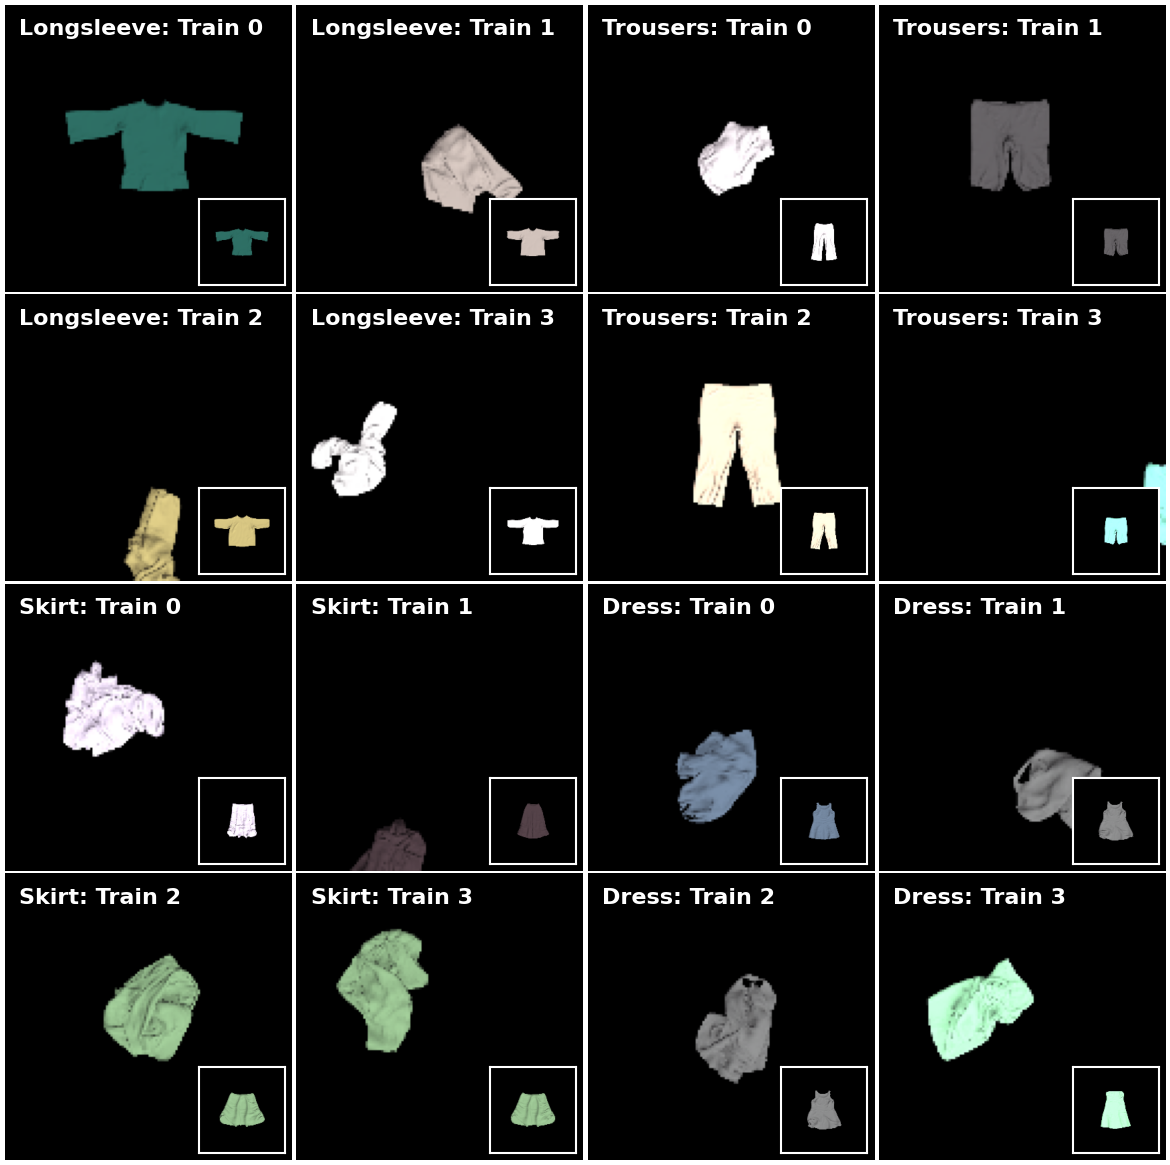
\includegraphics[width=1.0\linewidth]{plots/combined_garments_4x4_with_goals.png}\hfill
        \end{minipage}
    }
    % Second Subfigure: Real Garments
    \subfloat[Real garments used for real-world evaluation. \label{fig:real-garments}]{
        \begin{minipage}[c]{0.41\textwidth}
            \centering
            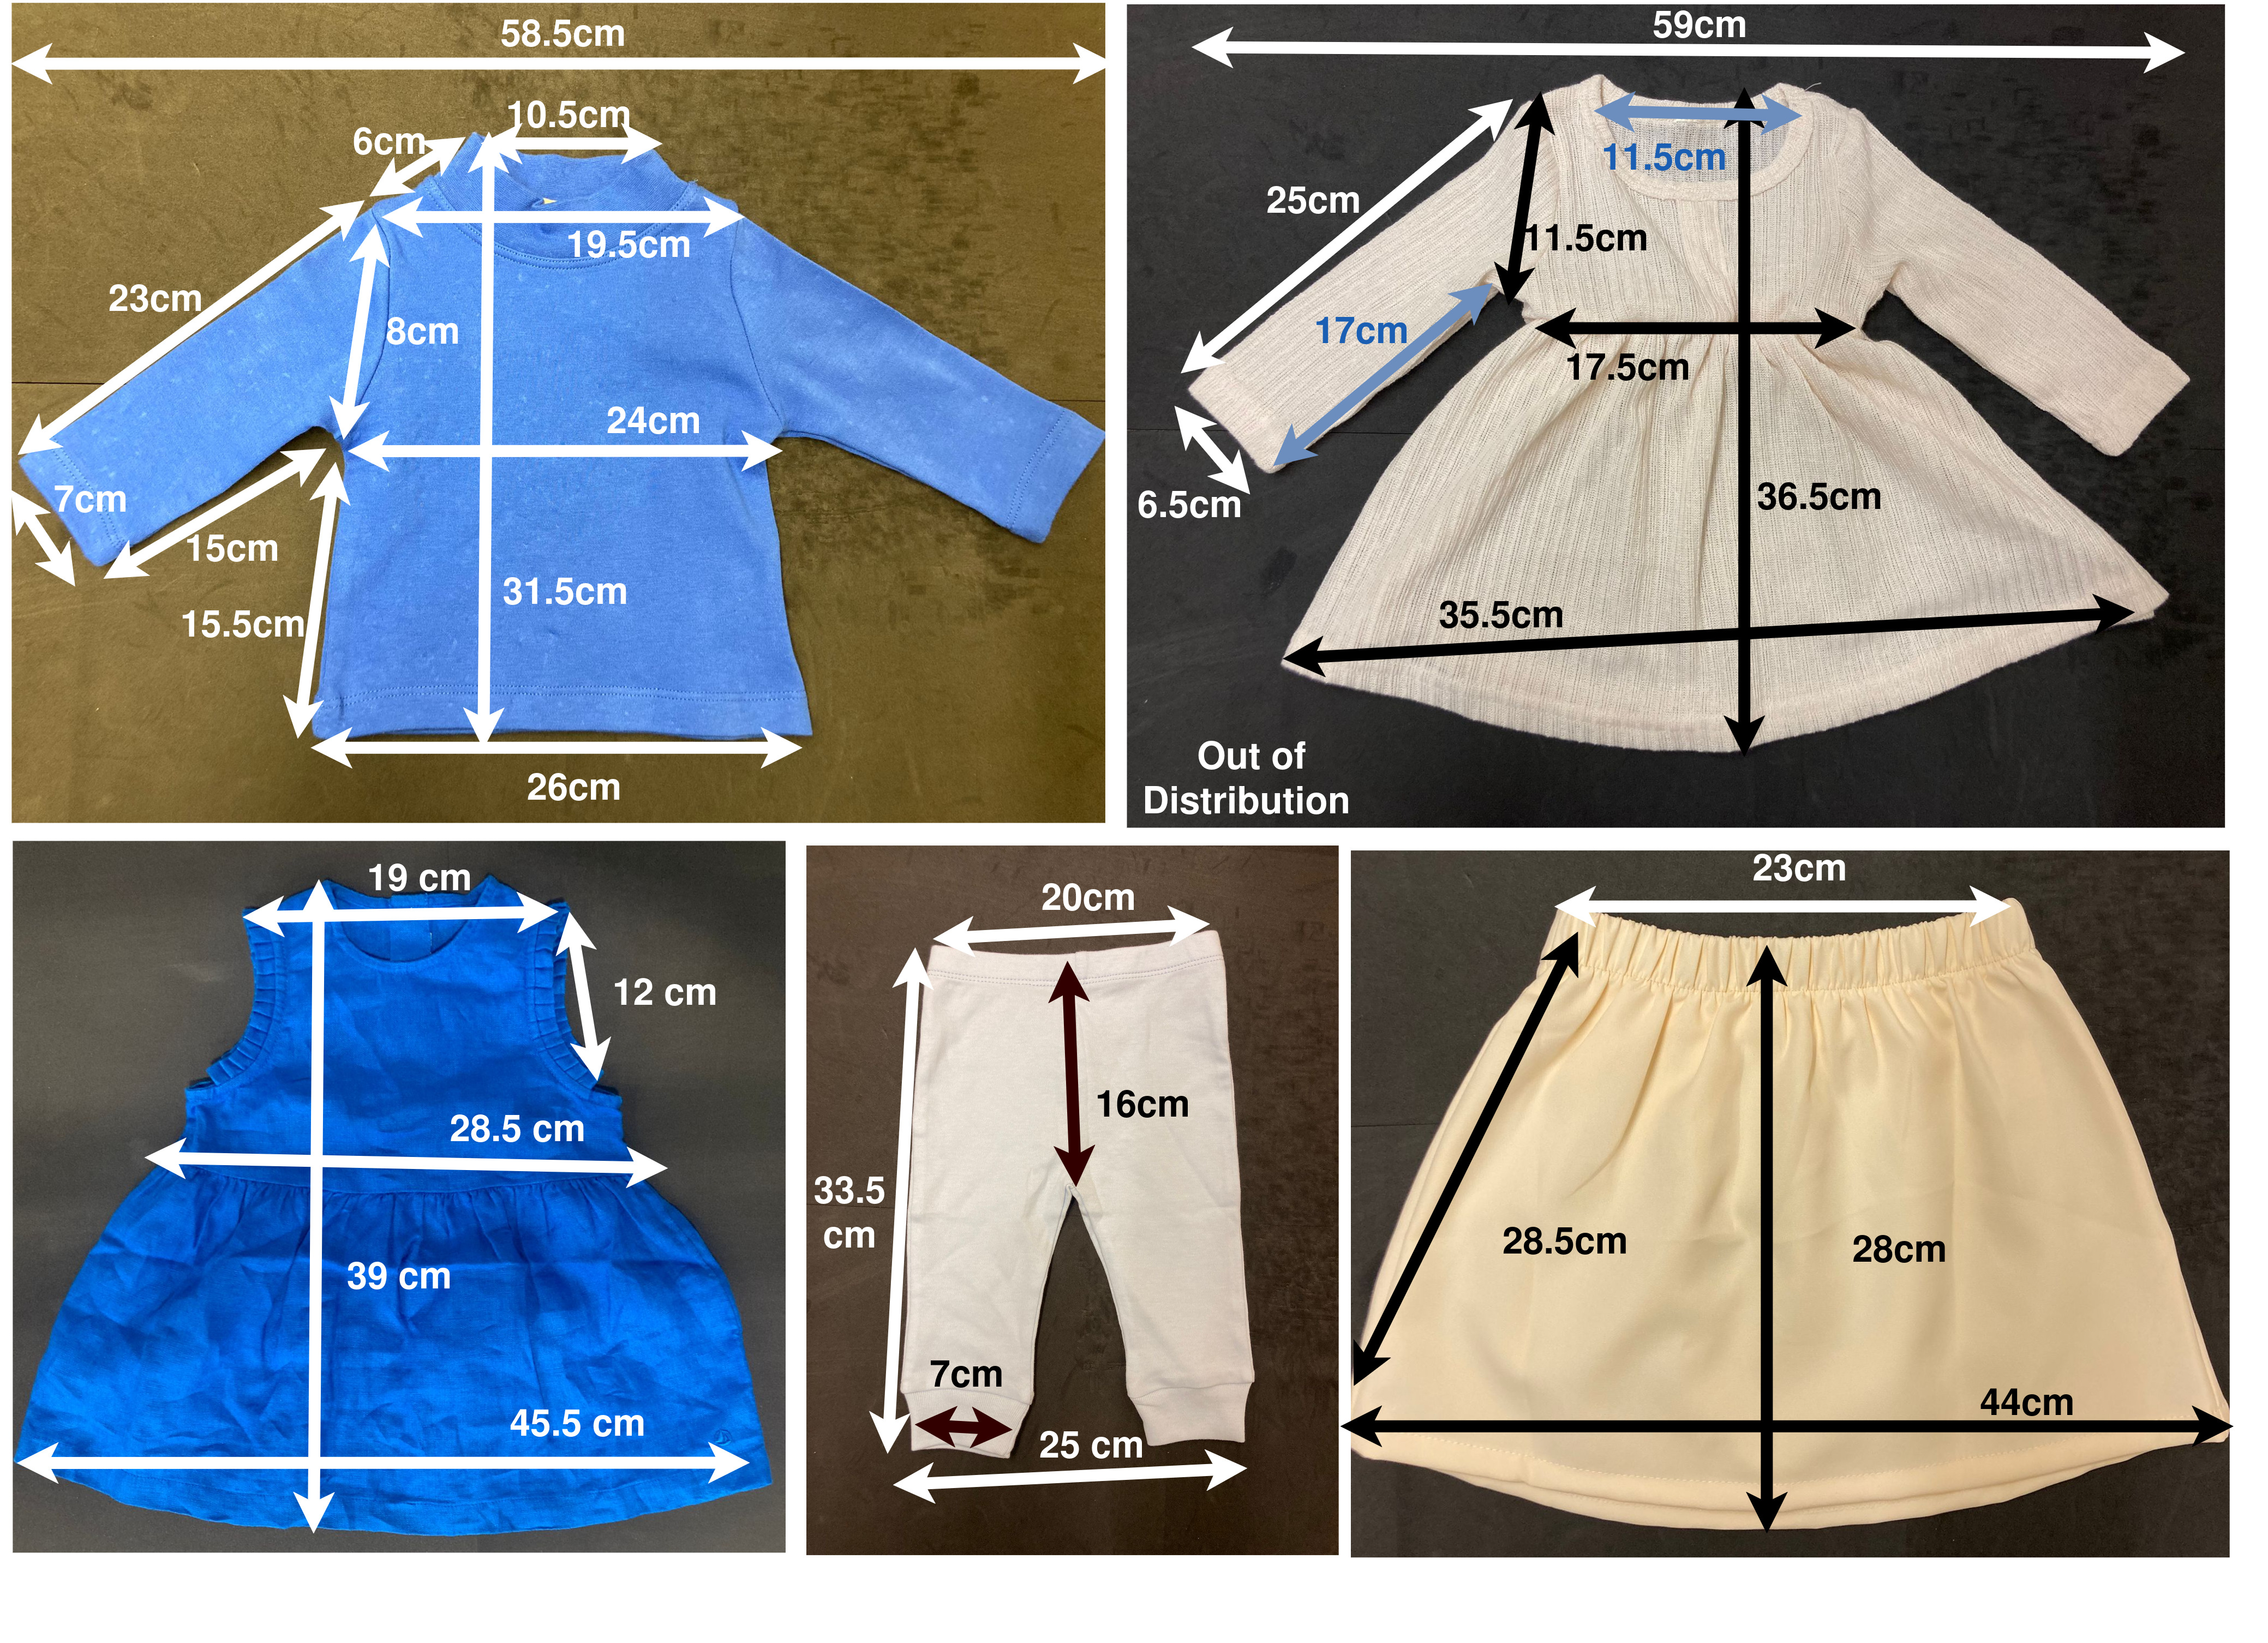
\includegraphics[width=1.0\linewidth]{plots/lagarnet-real-garments.jpg}
        \end{minipage}
    }
    % Second Subfigure: Real Garments
    \subfloat[UR5e Flattening a skirt  \label{fig:ur5e-onrobot}]{
        \begin{minipage}[c]{0.22\textwidth}
            \centering
            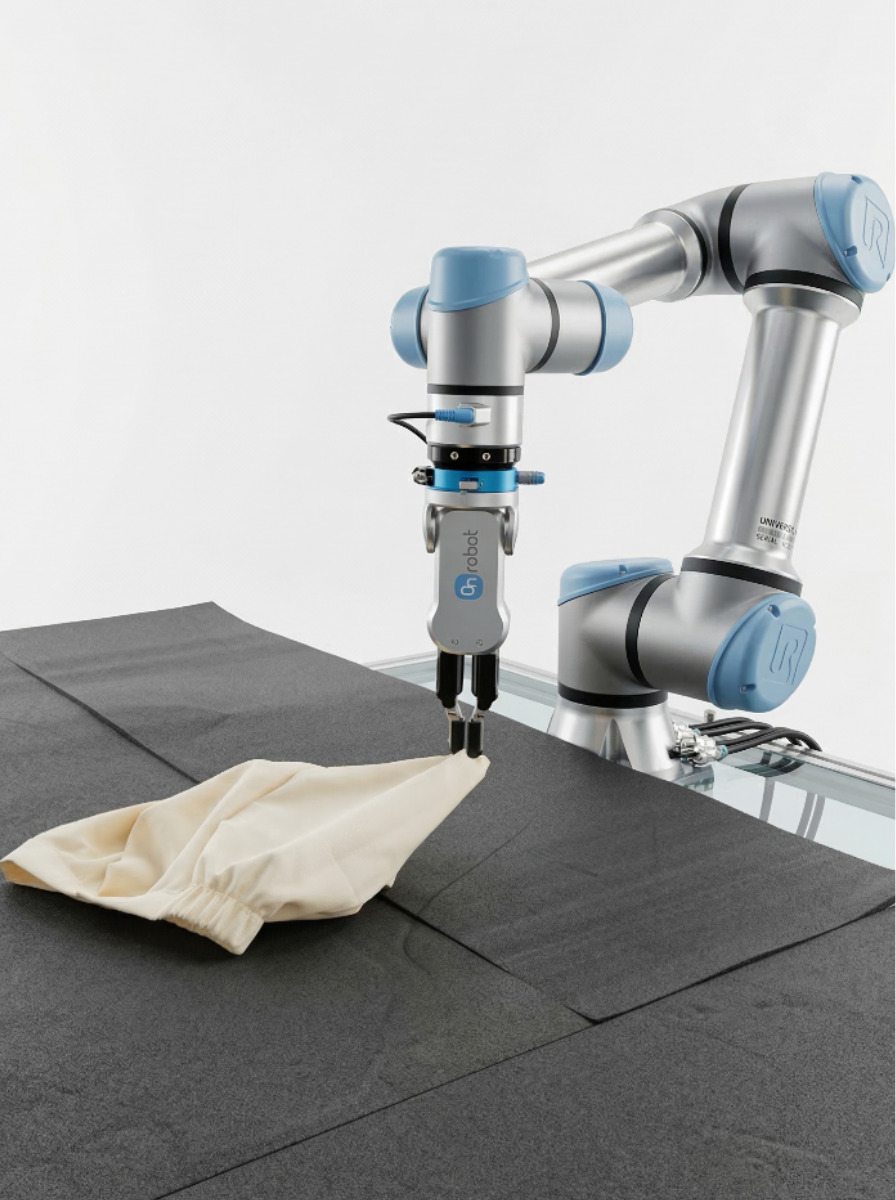
\includegraphics[width=1.0\linewidth]{plots/lagarnet-real-setup.jpg}
        \end{minipage}
    }
    
    \vspace{0.4cm} % Adds breathing room between the rows
    
    % --- ROW 2 ---
    
    % Third Subfigure: Spans the entire bottom row
    \subfloat[A qualitative demonstration of LaGarNet flattening a real dress.  \label{fig:ur3e-real-action-inference}]{
        \begin{minipage} [c]{0.98\textwidth}
            \centering
            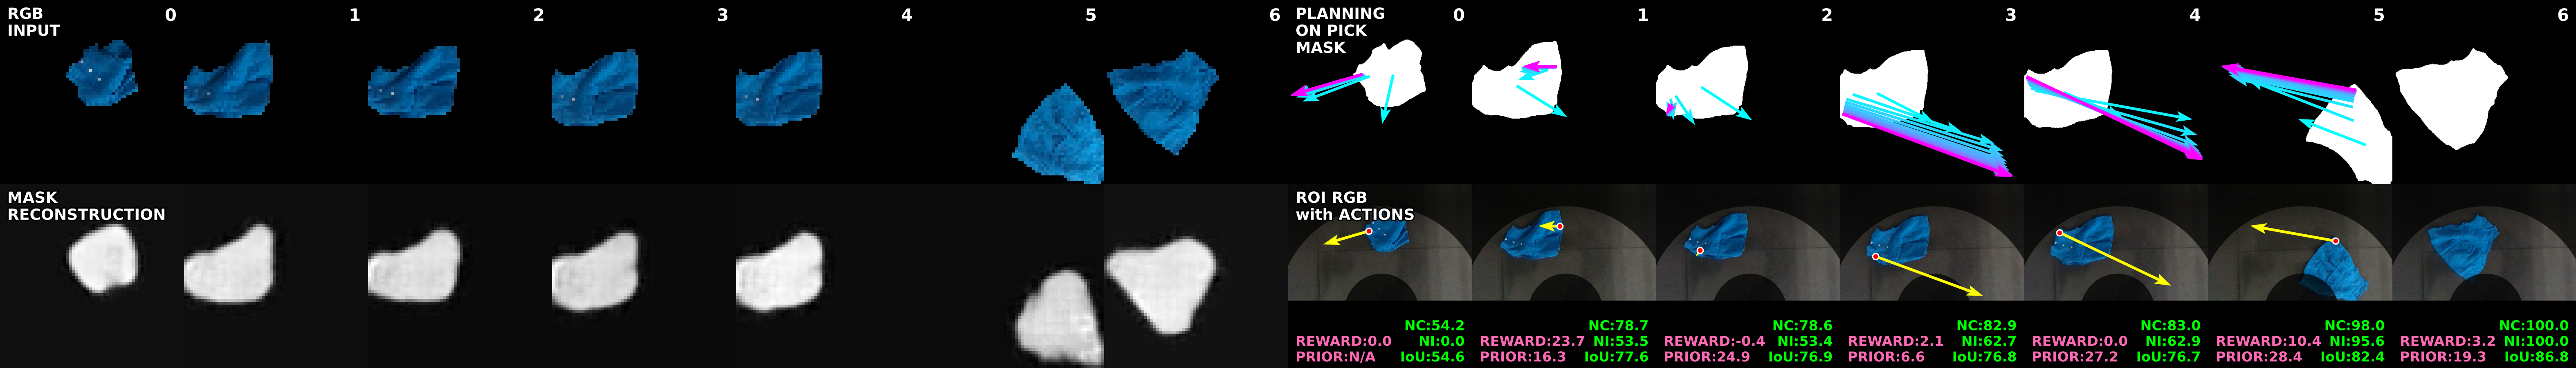
\includegraphics[width=1.0\linewidth]{plots/episode_4_combined.png}
        \end{minipage}
    }
    
    % Overall Figure Caption
    \caption{Overview of the experimental setup and qualitative results of LaGarNet. We train our \text{LaGarNet} policies on the dataset collected in simulation environments \cite{canberk2023cloth} and transfer them to \text{UR5e} real-world environments using the \text{DRAPER} deployment framework \cite{kadi2025draper} \addinfo{in a zero-shot manner}. (a) Initial states of synthetic garments with their goal states; from \text{Cloth3D} dataset \cite{bertiche2020cloth3d} simulated in \text{SoftGym} \cite{lin2020softgym}, our setup contains 200 training, 10 validation and 30 evaluation states. \addinfo{(b) The set of real garments used for UR5e physical evaluations; the blue longsleeved T-shirt consists of 95\% cotton and 5\% elastane; the blue dress is made from 100\% linen; the light-blue trousers are made of 100\% cotton; the khaki skirt is crafted from 100\% polyester; and, the beige dress is composed of 100\% cotton and features, the shape and material types are out of distribution learned on the training set.} (c) We use a UR5e robot arm with an OnRobot RG2 gripper (background removed and image quality enhanced using Google's Gemini 3 Flash Image). (d) Qualitative demonstration of the LaGarNet action inference process over successive steps on real dress; in the top right row, bright blue arrows represent the mean of the action Gaussian distribution in the early iteration stages, while the purple arrow represents the later resulting stages; the bottom right row demonstrates overall flattening effect of LaGarNet in a real-robot setup with normalised coverage (NC), maximum intersection-over-union (IoU), ground-truth reward (Reward), and predicted prior reward (Prior) from the last-step planning---all values are multiplied by 100.}
    \label{fig:LaGarNet}
\end{figure*}






% In addition, bi-manual manipulation on cloth-like objects introduces larger complexity in control presents many different types of failure modes \cite{gusseme2025insights}, whilst single-gripper PnP only suffers from misgrasping, multi-layer grasping as well as cloth slipping issues \cite{lin2022learning, hoque2022visuospatial}. The failures of PnP have been investigated and addressed from both hardware and control perspectives \cite{kadi2025draper, hoque2021lazydagger}. This paper aims to apply the \text{DRAPER} framework to more complex garment types, such as T-shirts, trousers, skirts and dresses as shown in Figure \ref{fig:sim-garments} and \ref{fig:real-garments}

% Single-gripper pick-and-place (\text{PnP})  has been empirically shown to be inferior to these hybrid actions \cite{ha2022flingbot, canberk2023cloth}, and this has impacted the field to move away from using a single robot arm. 

\addtypo{In this paper, we show that} our method \text{LaGarNet} can flatten four different types of complex garments, utilising the whole workspace of a robot arm in the real world (Figure \ref{fig:ur3e-real-action-inference}). \text{LaGarNet} \addadvantage{outperforms strong learning-based baselines such as PlaNet-ClothPick \cite{kadi2024planet} and Diffusion Policy \cite{chi2023diffusionpolicy}.  Moreover, it  matches the primary performance of mesh-based planning method, MEDOR \cite{huang2022mesh}, but with 17$\times$ faster inference time and 5$\times$ less network parameters. Most importantly, it slightly outperforms human-level performance within 10 steps in simulation.} \addinfo{Trained with simulated data and transferred to the real world in the zero-shot manner,} LaGarNet reaches on average 90\% NC, 80\% NI and 81\% Max IoU in our real-world experiments on examined garments displayed in Figure \ref{fig:real-garments}. In a nutshell, we make the following four contributions:

1. We propose a goal-conditioned recurrent state-space model (GC-RSSM) \addtypo{that enables} a single goal-conditioned garment-flattening planning method \text{LaGarNet} \addtypo{to} flatten garments in both simulation and real-world environments.

2. We \addtypo{develop} a general data-collection strategy for offline training of \text{PnP} garment-flattening controllers, which is a mixture of an expert \text{Diffusion Policy} learned from few human demonstrations and a masked-biased random policy.

3. We design a novel and effective coverage-alignment reward function for general garment flattening that can be calculated both in simulation and real-world environments.

4. We develop a workspace sampling and transfer heuristic to deploy the trained policy from a fixed square window observation space to a constrained environment limited by the  ring-shape workspace of robot arms for \text{PnP} primitives.

% Apart from the introduction (Section \ref{sec:introduction}) and the conclusion (Section \ref{sec:conclusion}), the remainder of this paper is organised as follows. Section \ref{sec:related-workd} presents the state-of-the-art development of garment flattening in robotics. Section \ref{sec:planet-clothpick++} details the proposed method, \text{LaGarNet}. Section \ref{sec:transfer-heuristic} describes the transfer heuristic employed to bridge the gap between simulation and real-world observation-action space. Section \ref{sec:experiments} presents both simulation, real-world experimental results and a set of detailed ablation studies, along with corresponding analyses. Finally, Section \ref{sec:discussion} addresses the current limitations of our approach and outlines potential directions for future research.


\section{Related Work} \label{sec:related-workd}


\noindent Applications of learning-based methods on cloth-shaping tasks, i.e., flattening and folding cloth-like objects, include \text{model-free reinforcement learning} \cite{matas2018sim,wu2020learning,ha2022flingbot,hietala2022learning,lin2020softgym,lee2021learning, canberk2023cloth, he2024fabricfolding, gu2023learning, avigal2022speedfolding}, \text{model-based reinforcement learning} \cite{yan2021learning,hoque2022visuospatial,ma2021learning,arnold2023cloth,lin2020softgym,lin2022learning, huang2022mesh} and  \text{behaviour cloning} \cite{lips2024learning,weng2022fabricflownet, teng2022multidimensional, mo2022foldsformer, huang2025sis, chi2023diffusionpolicy} algorithms. Many successful learning-based  controllers employ intermediate explicit representations to assist downstream controllers to mitigate the server self-occlusion problem of cloth. These encompass key-point detection \cite{lips2024learning, gusseme2025insights}, seam feature extraction \cite{huang2025sis}, mesh reconstruction \cite{huang2022mesh} as well as optical flow \cite{weng2022fabricflownet} and dense visual correspondence between current and goal images \cite{wu2024unigarmentmanip}. In contrast, our work focuses on learning a latent dynamic representation and generating actions through planning, making our method generalisable to different scenarios.

These systems also vary in terms of action space. While some methods attempt low-level position/velocity control \cite{matas2018sim,lin2020softgym, hietala2022learning,ha2022flingbot}, others adopt  \text{pick-and-fling} (PnF) action primitives \cite{doumanoglou2014autonomous}, \text{pick-and-place} (PnP)  \cite{sun2015accurate}, and \text{pick-and-drag} (PnD) primitives \cite{he2024fabricfolding} to achieve cloth shaping. Some  approaches that uses hybrid of the aforementioned three primitives have demonstrated significant efficacy of such complex action spaces in facilitating diverse garment manipulation tasks \cite{avigal2022speedfolding, canberk2023cloth}. However, the incorporation of these hybrid strategies introduces additional complexity to the action space for data collection and control itself. Single-gripper PnP only suffers from misgrasping, multi-layer grasping and cloth slipping issues \cite{lin2022learning, hoque2022visuospatial}; it has been investigated and addressed from both hardware and control perspectives \cite{kadi2025draper, hoque2021lazydagger}. In this paper, we focus on PnP primitives and put the focus on the learning aspects of the latent dynamic model.

\subsection{Model-Based Methods in Cloth Shaping} \label{sec:mbrl}

The use of cloth dynamics is prevalent in reinforcement learning approaches; learning and using such dynamics can improve data efficiency of policy training and improve the precision of actions during inference time \cite{hafner2019learning, hafner2025mastering, kadi2024planet, lin2022learning}. It is also effective for goal-conditioned tasks \cite{duan2024learning, hoque2022visuospatial}, as we can exploit the distance between current and goal states for planning. The model-based methods in this domain can be classified into mesh-based and mesh-free methods, depending if the cloth-mesh reconstructed during test time.

Most model-based methods focus on reconstructing a 3D mesh and mesh dynamic of the target cloth \cite{huang2022mesh, lin2022learning, tian2025diffusion}. For example, \text{Visible Connectivity Dynamics (VCD)} \cite{lin2022learning} first applies such mesh models  on the visible part of the cloth to achieve more precise planning. Building on \text{VCD}, Huang et al.~\cite{huang2022mesh} also adopt point clouds as input for mesh reconstruction and planning in the mesh-dynamic space; their method \text{MEDOR}  explicitly reconstructs the occluded part of the cloth from a top-down camera by fine-tuning an initial reconstructed mesh in real time based on the template of the target garment. 

On the other hand, the mesh-free model-based approach \text{Contrastive Forward Modelling (CFM)} \cite{yan2021learning} trains latent dynamics for planning applications. Hoque et al.~\cite{hoque2022visuospatial} proposed \text{Visual Foresight Modelling (VSF)}, which integrates variational video prediction models within the \text{Visual MPC} framework \cite{ebert2018visual} to address model exploitation. Nevertheless, \text{VSF} has demonstrated limited efficacy in garment-flattening applications \cite{lin2022learning} and neither of these mesh-free planning methods have  managed to match the performance of mesh-based \text{VCD} \cite{lin2022learning}.  In contrast, our proposed mesh-free planning method \text{LaGarNet} matches the state-of-the-art performance the above mesh-based methods on flattening tasks while having a smaller numbers of parameters and faster inference time.

As a mesh-free method, \text{Deep Planning Network (PlaNet)} \cite{hafner2019learning} has been widely studied in control tasks \cite{yan2021learning, ma2021learning, lin2020softgym}, but has also shown limited efficacy in deformable object manipulation. This is attributed to blurred visual reconstructions that loses edge and corner details critical for shaping \cite{yan2021learning, hoque2022visuospatial, lin2022learning}. \text{PlaNet-ClothPick} \cite{kadi2024planet}, a cloth-flattening algorithm based on a \addtypo{recurrent state-space model (RSSM)}, mitigates this by restricting pick actions to the cloth mask, designing a flattening-specific reward, and using an engineered offline dataset. While it achieves perfect flattening in simulation and over 70\% NC on real towels \cite{kadi2024planet, kadi2025draper}, it fails to generalise to complex garments due to strong inductive biases. Our single-policy \text{LaGarNet} reduces these biases through a general data-collection procedure and coverage-alignment reward, enabling robust garment flattening.

Lastly, model-based methods leverage the difference between current and goal observations to generate reward signals for cloth shaping \cite{hoque2022visuospatial, yan2021learning}. Arnold et al.~\cite{arnold2023cloth} extend this idea to mesh-level goal-conditioned policies for complex tasks, but their method remains limited to fabric manipulation. Model-free approaches train goal-conditioned representations \cite{mo2022foldsformer}, flow networks \cite{weng2022fabricflownet}, or use \text{Hindsight Replay Buffer} \cite{andrychowicz2017hindsight, lee2021learning}, yet are restricted to simple fabrics. In contrast, we propose a goal-conditioned RSSM (GC-RSSM) that predicts step-wise flattening rewards and achieves garment flattening across four types: longsleeved T-shirts, trousers, skirts, and dresses.




\subsection{Reward Functions in Cloth Shaping} \label{sec:reward-literature}
Reward engineering is an essential component for the success of a reinforcement learning (RL) controller. Many RL algorithms in garment-flattening systems come with their own reward function \cite{canberk2023cloth, gu2023learning, avigal2022speedfolding}. \text{ClothFunnels} \cite{canberk2023cloth} adopts a canonicalisation-alignment reward  function $\mathcal{R}_{NA}$  which is a linear interpolation of normalised delta deformation distance for alignment $\mathcal{R}_{dA}$ and normalised delta rigid distance for canonicalisation $\mathcal{R}_{dN}$, i.e., $\mathcal{R}_{NA} = \alpha\mathcal{R}_{dN} + (1-\alpha)\mathcal{R}_{dA}$. \text{Learning2Unfold} \cite{gu2023learning} employs a coverage-orientation reward $\mathcal{R}_{CO}$ that has the similar interpolation between the normalised coverage $\mathcal{R}_C$ and the orientation $\mathcal{R}_o = 1 - tanh^2\theta$, where $\theta = \alpha|\theta_P| + (1-\alpha)|\theta_F|$; the $\theta_P$ represents the angle between the current cloth and goal cloth and $\theta_F$ represent the flipping angle $\theta_F$ to assure the cloth is facing down. 


\text{SpeedFolding} \cite{avigal2022speedfolding} uses a coverage-smoothness reward function $\mathcal{R}_{CS}$ that mixes the delta coverage $\mathcal{R}_{dC} = NC_t - NC_{t-1}$ and delta smoothness estimation $\Tilde{R}_{dS}$ between the current and the last frame, then clip reward between 0 and 1 after a tanh scaling, i.e., $\mathcal{R}_{CS} = max(tanh(\alpha*\mathcal{R}_{dC} + \beta*\Tilde{R}_{dS}), 0)$; note that the smoothness estimation is inferred through a pre-trained smoothness prediction network. \text{PlaNet-ClothPick} employs a specially engineered reward function based on \text{VSF}'s reward specifically for the fabric-flattening task \cite{hoque2022visuospatial}. In this study, we propose a new reward function coverage-alignment $\mathcal{R}_{CA}$ that simplifies the \text{SpeedFolding}'s coverage-smoothness reward $\mathcal{R}_{CS}$ \cite{avigal2022speedfolding}. Note that, unlike \text{ClothFunnels}'s canonicalisation-alignment reward which needs to calculate particle-wise distances, which requires an oracle, our reward function should, in theory, work for both simulation and real-world learning.

% \begin{figure}[t!]
%     \centering
%     \subfloat[\centering Human Policy Trajectory \label{fig:human-tshirt-demo}] {{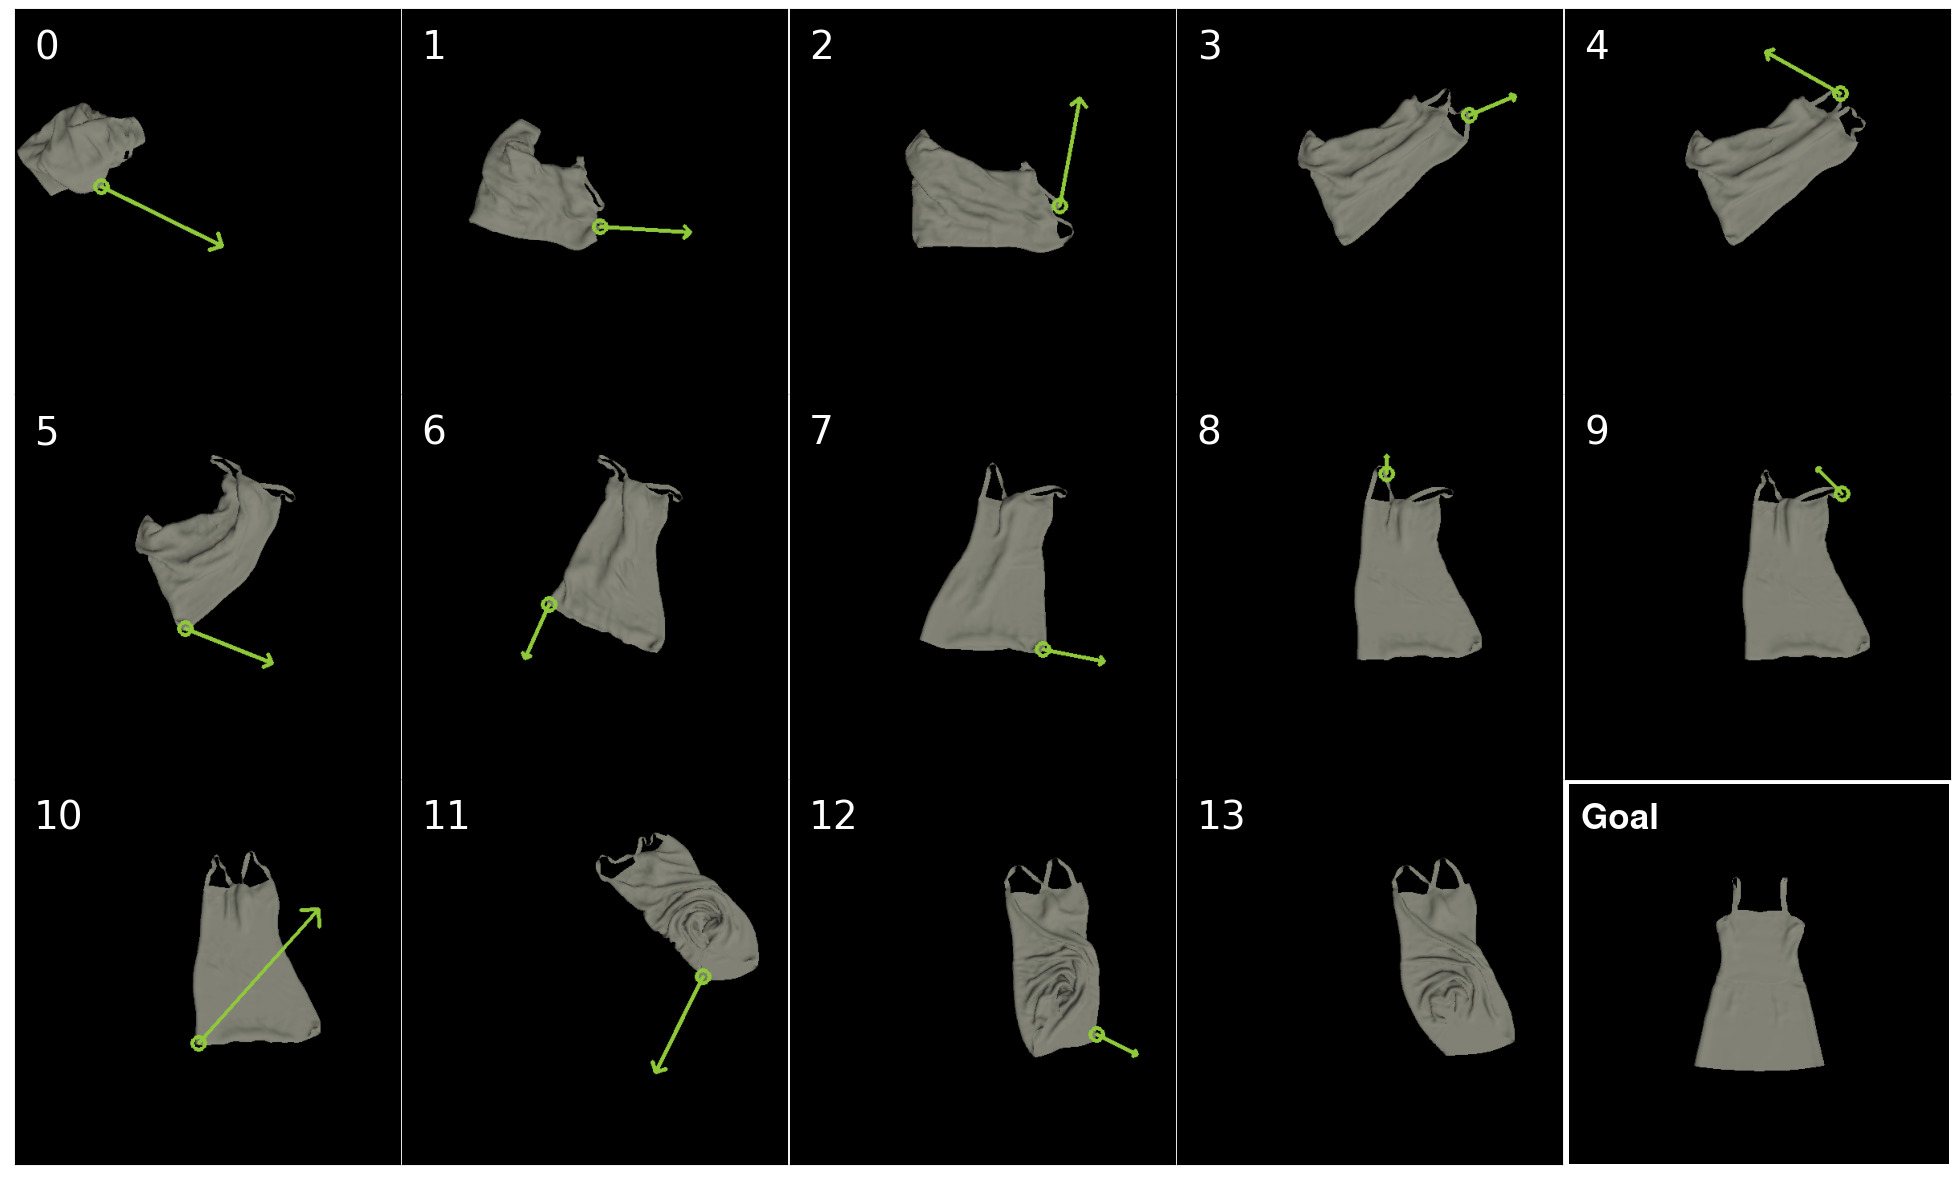
\includegraphics[width=0.27\textwidth]{plots/huam-trj-with-goal.jpg} }}
%     \subfloat[\centering Rewards \label{fig:reward-diff}] {{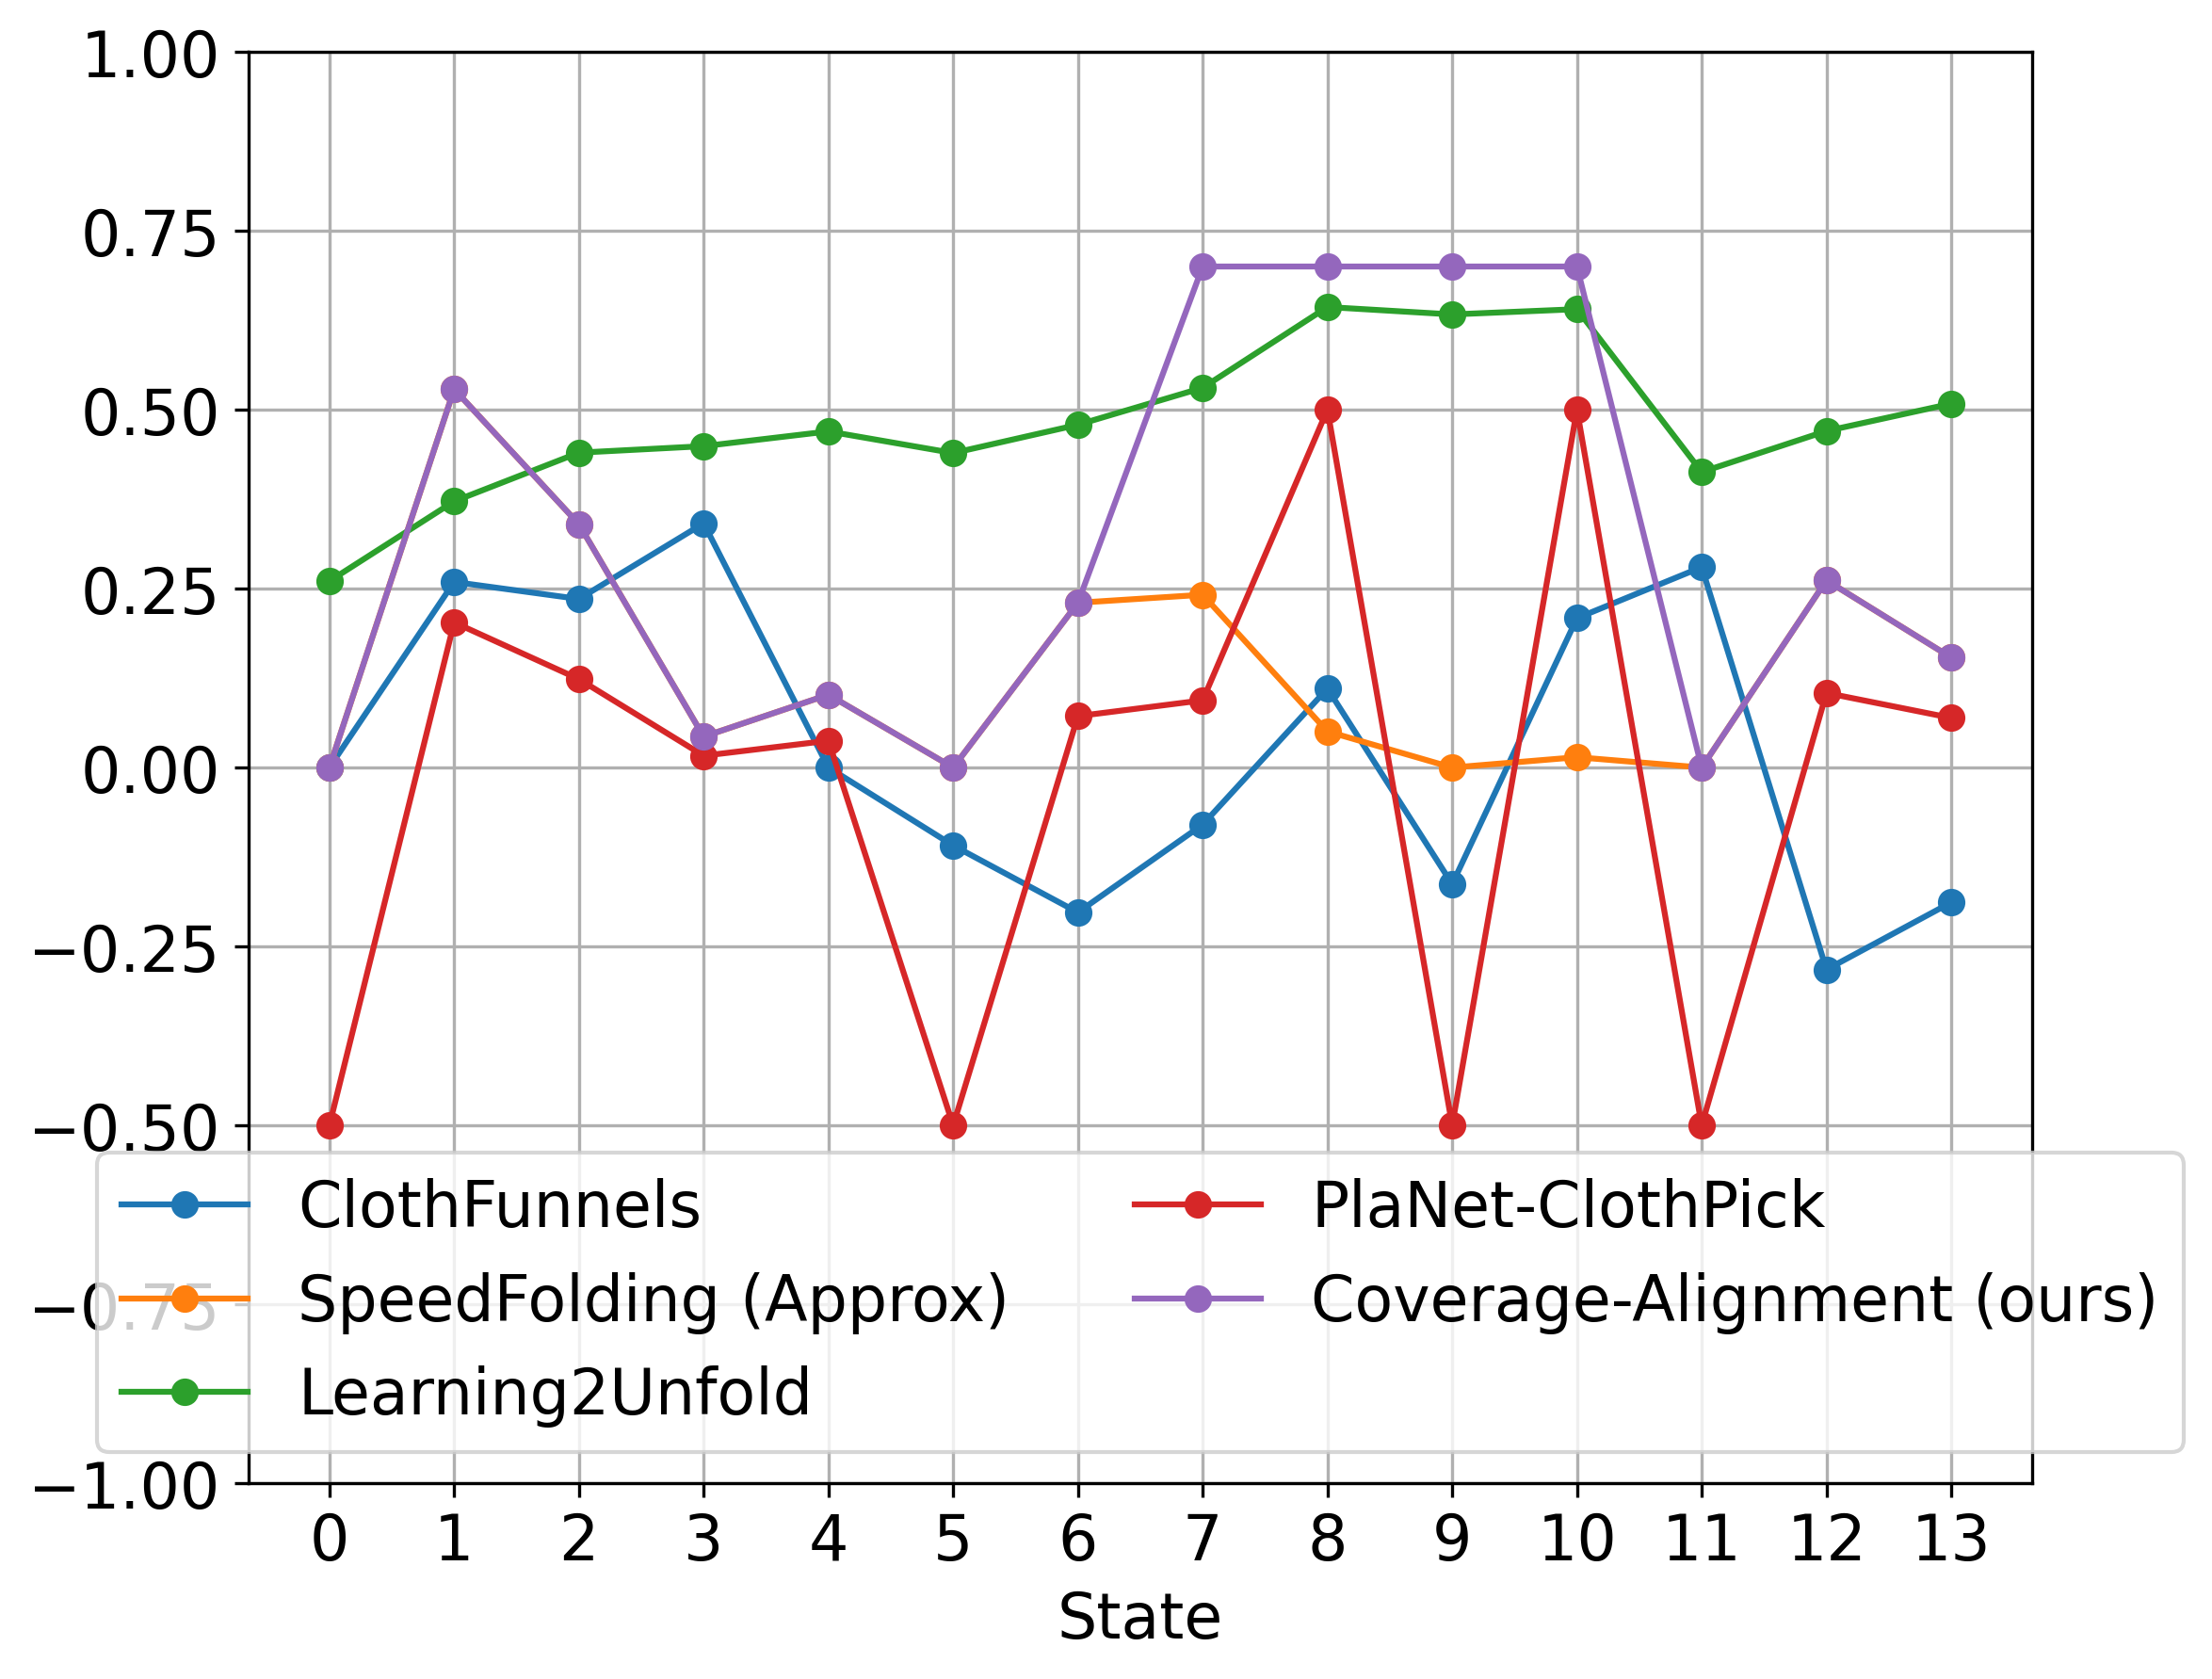
\includegraphics[width=0.22\textwidth]{plots/human-rewards.png} }}
%     \caption{Rewards of human policy in flattening a simulated dress. Figure (a) demonstrates the trajectory rollout of a human policy; Figure (b) shows the step-wise comparison of the reward function; and Figure (c) indicates the changes of different evaluation metrics for flattening. \texttt{SpeedFolding (Approx)} is the basis our initial coverage-alignment reward, where we use difference of Max IoU to replace the smoothness estimation. \texttt{Coverage-Alignment (ours)} is our final reward function with bonus and penality augmentaiton.}
% \end{figure}


\subsection{Data Collection and Preparation}

The high-dimensional state-action space of deformable objects makes it challenging to train policy representations, dynamics models or value functions. Moreover, model-based methods in cloth-shaping tasks often suffer from model exploitation (choosing actions the model incorrectly estimates as optimal) and compounding error (accumulated errors in imagined roll-outs). The effectiveness of a learned world model depends on how diverse and comprehensive the trajectory data are in the training dataset \cite{duan2024learning}. Training typically requires a large amount of data collected with carefully designed blends of policies \cite{hoque2022visuospatial, yan2021learning, ma2021learning, kadi2024planet}. To address this, prior work has used demonstration data \cite{matas2018sim,hoque2022visuospatial}, corner-biased sampling \cite{hoque2022visuospatial,weng2022fabricflownet} (biasing pick actions toward fabric corners and edges), and other engineered strategies \cite{arnold2023cloth,lin2022learning}. However, these approaches impose strong inductive biases on the learning algorithm. In contrast, our study proposes a general data collection procedure based on a Diffusion Policy \cite{chi2023diffusionpolicy} trained from a few human demonstrations and a random oracle policy, which empirically yields effective training data for MBRL algorithms.


\subsection{Goal-Conditioned Methods using RSSM}
Some previous research attempted to integrate goal-conditioned learning in RSSMs. Pertsch et al.~ \cite{pertsch2020long} proposed a goal-condition predictor \text{(GCP)} that conditioned on the initial and goal states of subtask of a long horizon tasks, and they further improve the planning by using a hierarchical divide-and-conquer scheme; the action is inferred inversely from current and an optimised sub-goal. Duan et al. ~\cite{duan2024learning} present a goal-directed exploration algorithm, \text{MUN}, and they also devise \text{GC-Dreamer} as a baseline to compare against \text{MUN}; but the goal of \text{GC-Dreamer} is conditioned on the actor and the critic network instead of the world model. Our method is different from these method because we condition the goal directly on the latent state inference of RSSM for learning better representation.



% \subsection{Action Inference in Cloth Shaping}


% Learning-based approaches using high-level action primitives for cloth-shaping tasks generally adopts two strategies to learn the action: continuous action inference and state-action value map.

% \subsubsection{Continuous Action Inference}
% Early vision-based learning methods for continuous action inference, such as \cite{matas2018sim} and \cite{yan2021learning}, have studied many model-free reinforcement learning algorithms for pixel-based pick-and-place (\text{PnP}) action primitives on fabrics. One technique that leads to better \text{PnP} continuous action policy learning is the separation of the inference of pick and place positions; \cite{wu2020learning} suggest using \text{Maximum Value of Placing} that selects the best picking position after choosing the best placing position. \text{Diffusion Policy} \cite{chi2023diffusionpolicy} adapted to PnP domain \cite{kadi2025draper} with continuos action inference demonstrated a promising performance on towel flattening and folding in the real world. In this paper, we choose the diffusion policy as a candidate of imitation learning methods that uses continuos action inference. Research community have generally drifted toward discretised action-space using the following state-action value maps for further performance improvement on garments, as it facilitates effective masking of high-level action primitives.

% \subsubsection{State-Action Value Map} Discretising \text{PnP} action space is a common technique in cloth-shaping literature for model-free reinforcement learning  methods. A prevalent strategy for garment manipulation is using state-action value map (\text{SAVM}), where a convolutional auto-encoder produces value heatmaps on observation images. Lee et al.~\cite{lee2021learning} first propose the use of \text{SAVM} in fabric manipulation tasks by rotating and scaling the observation image and stacking them channel-wise as input to a network. Their system, trained in the real world with goal-conditioned offline \text{Deep Q-Learning} \cite{mnih2013playing}, successfully achieves several fabric folding tasks. They examine six folding tasks, achieving perfect success rates for four easier folds but struggling with more complex ones. Building on this Rotate-Scale \text{SAVM} (RS-\text{SAVM}), \text{FlingBot} \cite{ha2022flingbot} employs dual robot arms for fling primitives, using online \text{RL} in simulation before fine-tuning in the real world with pre-collected data to enhance flattening performance. 

% Extending on \text{FlingBot}, \text{ClothFunnels} \cite{canberk2023cloth} introduces a canonicalised-alignment objective to align garments with a predefined configuration, combining \text{PnP} and \text{pick-and-fling} primitives via RS-\text{SAVM} decoders and corresponding encoders. \text{FabricFolding} \cite{he2024fabricfolding} further adds a \text{Pick-and-Drag} primitive, where one gripper stays stationary while the other performs a dragging motion, alongside a key-point detection network for transitioning from flattening to a heuristic folding policy \cite{canberk2023cloth}. Similarly, \text{Learning2Unfold} \cite{gu2023learning} builds on \text{ClothFunnels} using a key-point detection network to provide grasping masks for RS-\text{SAVM}s. Diverging from rotation-scaling channels, \text{SpeedFolding} \cite{avigal2022speedfolding} uses a \text{U-Net} \cite{ronneberger2015u} to generate \text{SAVM}s by directly predicting key pixel values for place, fling, and drag actions. Their system, trained with a hybrid of offline and online \text{RL}, achieves nearly 10x speed-up over prior works \cite{doumanoglou2016folding, maitin2010cloth}. 

% In contrast, \text{JA-TN} \cite{kadi2024mjtn}, a behaviour cloning method building on \text{TransporterNet} \cite{zeng2021transporter}, infers direct \text{SAVM} and demonstrates high performance on single-gripper \text{PnP} towel shaping in both simulation and the real world. DRAPER \cite{kadi2025draper} demonstrate that the real-world deployed \text{JA-TN} can achieve above 87\% \text{NC} and  82\% \text{NI} on flattening rectangular fabrics with various types of materials. In this paper, we also investigates the performance of \text{JA-TN} on complex garment flattening tasks. Also, we choose the off-the-shelf \text{ClothFunnels} as the reinforcement learning  representative that uses SAVM action inference.


\section{LaGarNet} \label{sec:planet-clothpick++}

\begin{figure*}[t!]
    \centering
    
    % --- Subpart (a): Real Robot Setup ---
    \begin{subfigure}[t]{0.98\linewidth}
        \centering
        \tikz{
 % ================== CUSTOM STYLES ==================
 \tikzset{
   half-half/.style={
     path picture={
       \fill[orange!40] (path picture bounding box.south west) rectangle (path picture bounding box.north);
       \fill[red!80] (path picture bounding box.south) rectangle (path picture bounding box.north east);
     }
   }
 }

 % ================== NODES ==================
 % We group the nodes by time step. 
 % All spacing has been increased by 1.5x for a wider layout.

 % ------ t = 0 (Initial State) ------
 \node[latent, minimum size=0.8cm, fill=orange!40] (z0) {$\boldsymbol{z}_0$};
 \node[latent, rectangle, minimum size=0.8cm, above=0.6cm of z0] (h0) {$\boldsymbol{0}$};
 \node[obs, minimum size=0.8cm, above=0.6cm of h0] (a0) {$\boldsymbol{a}_{\text{no-op}}$}; 
 
 % y1 and r1 directly under z0
 \node[latent, minimum size=0.8cm, below=0.6cm of z0, fill=blue!40] (y0) {$\boldsymbol{y}_1$};
 \node[latent, minimum size=0.8cm, below=0.25cm of y0, fill=blue!40] (r0) {$\boldsymbol{r}_1$};
 
 % ------ t = 1 ------
 \node[latent, minimum size=0.8cm, right=1.8cm of z0, half-half] (z1) {$\boldsymbol{z}_1$};
 \node[latent, rectangle, minimum size=0.8cm, above=0.6cm of z1] (h1) {$\boldsymbol{h}_{1}$};
 \node[obs, minimum size=0.8cm, above=0.6cm of h1] (a1) {$\boldsymbol{a}_1$}; 
 
 \node[latent, minimum size=0.8cm, below=0.6cm of z1, fill=blue!40] (y1) {$\boldsymbol{y}_1$};
 \node[latent, minimum size=0.8cm, below=0.25cm of y1, fill=blue!40] (r1) {$\boldsymbol{r}_1$};
 
 % g and x scaled to 0.35cm left
 \node[obs, minimum size=0.8cm, left=0.35cm of z1, fill=green!30] (g1) {$\boldsymbol{g}$};
 \node[obs, minimum size=0.8cm, left=0.35cm of y1, fill=purple!30] (x1) {$\boldsymbol{x}_1$};

 % ------ t = 2 ------
 \node[latent, minimum size=0.8cm, right=1.8cm of z1, half-half] (z2) {$\boldsymbol{z}_2$};
 \node[latent, rectangle, minimum size=0.8cm, above=0.6cm of z2] (h2) {$\boldsymbol{h}_{2}$};
 \node[obs, minimum size=0.8cm, above=0.6cm of h2] (a2) {$\boldsymbol{a}_2$}; 
 
 \node[latent, minimum size=0.8cm, below=0.6cm of z2, fill=blue!40] (y2) {$\boldsymbol{y}_2$};
 \node[latent, minimum size=0.8cm, below=0.25cm of y2, fill=blue!40] (r2) {$\boldsymbol{r}_2$};
 
 \node[obs, minimum size=0.8cm, left=0.35cm of z2, fill=green!30] (g2) {$\boldsymbol{g}$};
 \node[obs, minimum size=0.8cm, left=0.35cm of y2, fill=purple!30] (x2) {$\boldsymbol{x}_2$};

 % ------ t - 1 ------
 \node[latent, minimum size=0.8cm, right=1.8cm of z2, half-half] (zt) {$\boldsymbol{z}_{t-1}$};
 \node[latent, rectangle, minimum size=0.8cm, above=0.6cm of zt] (ht) {$\boldsymbol{h}_{t-1}$};
 \node[obs, minimum size=0.8cm, above=0.6cm of ht] (at) {$\boldsymbol{a}_{t-1}$}; 
 
 \node[latent, minimum size=0.8cm, below=0.6cm of zt, fill=blue!40] (yt) {$\boldsymbol{y}_{t-1}$};
 \node[latent, minimum size=0.8cm, below=0.25cm of yt, fill=blue!40] (rt) {$\boldsymbol{r}_{t-1}$};
 
 \node[obs, minimum size=0.8cm, left=0.35cm of zt, fill=green!30] (gt) {$\boldsymbol{g}$};
 \node[obs, minimum size=0.8cm, left=0.35cm of yt, fill=purple!30] (xt) {$\boldsymbol{x}_{t-1}$};

 % ------ t ------
 \node[latent, minimum size=0.8cm, right=1.8cm of zt, half-half] (zt1) {$\boldsymbol{z}_{t}$};
 \node[latent, rectangle, minimum size=0.8cm, above=0.6cm of zt1] (ht1) {$\boldsymbol{h}_{t}$};
 \node[latent, minimum size=0.8cm, above=0.6cm of ht1, fill=yellow!30] (at1) {$\boldsymbol{a}_{t}$}; 
 
 \node[latent, minimum size=0.8cm, below=0.6cm of zt1, fill=blue!40] (yt1) {$\boldsymbol{y}_{t}$};
 \node[latent, minimum size=0.8cm, below=0.25cm of yt1, fill=blue!40] (rt1) {$\boldsymbol{r}_{t}$};
 
 \node[obs, minimum size=0.8cm, left=0.35cm of zt1, fill=green!30] (gt1) {$\boldsymbol{g}$};
 \node[obs, minimum size=0.8cm, left=0.35cm of yt1, fill=purple!30] (xt1) {$\boldsymbol{x}_{t}$};

 % ------ t + 1 (No x node) ------
 \node[latent, minimum size=0.8cm, right=1.8cm of zt1, fill=red!80] (zt2) {$\boldsymbol{z}_{t+1}$};
 \node[latent, rectangle, minimum size=0.8cm, above=0.6cm of zt2] (ht2) {$\boldsymbol{h}_{t+1}$};
 \node[latent, minimum size=0.8cm, above=0.6cm of ht2, fill=yellow!30] (at2) {$\boldsymbol{a}_{t+1}$}; 
 
 \node[latent, minimum size=0.8cm, below=0.6cm of zt2, fill=blue!15] (yt2) {$\boldsymbol{y}_{t+1}$};
 \node[latent, minimum size=0.8cm, below=0.25cm of yt2, fill=blue!15] (rt2) {$\boldsymbol{r}_{t+1}$};
 
 \node[obs, minimum size=0.8cm, left=0.35cm of zt2, fill=green!30] (gt2) {$\boldsymbol{g}$};

 % ------ T (No x node) ------
 \node[latent, minimum size=0.8cm, right=1.8cm of zt2, fill=red!80] (zT) {$\boldsymbol{z}_T$};
 \node[latent, rectangle, minimum size=0.8cm, above=0.6cm of zT] (hT) {$\boldsymbol{h}_{T}$};
 \node[latent, minimum size=0.8cm, above=0.6cm of hT, fill=yellow!30] (aT) {$\boldsymbol{a}_{T}$}; 
 
 \node[latent, minimum size=0.8cm, below=0.6cm of zT, fill=blue!15] (yT) {$\boldsymbol{y}_{T}$};
 \node[latent, minimum size=0.8cm, below=0.25cm of yT, fill=blue!15] (rT) {$\boldsymbol{r}_{T}$};
 
 \node[obs, minimum size=0.8cm, left=0.35cm of zT, fill=green!30] (gT) {$\boldsymbol{g}$};

 % ================== EDGES ==================

 % 1. Generation of h (ORANGE)
 \edge[black, very thick] {a0, h0, z0} {h1} 
 \edge[black, very thick] {a1, h1, z1} {h2} 
 \edge[black, very thick] {at, ht, zt} {ht1} 
 \edge[black, very thick] {at1, ht1, zt1} {ht2}
 
 % 2. Generation of y and r (BLUE)
 % Vertical edges
 \edge[blue, very thick] {z0}{y0} \edge[blue, very thick] {z1}{y1} \edge[blue, very thick] {z2}{y2} 
 \edge[blue, very thick] {zt}{yt} \edge[blue, very thick] {zt1}{yt1} \edge[blue, very thick] {zt2}{yt2} \edge[blue, very thick] {zT}{yT}
 
 % Curved edges
 \path (z0) edge [bend left=45, ->, blue, very thick] (r0); \path (h0) edge [bend left=45, ->, blue, very thick] (y0); \path (h0) edge [bend left=45, ->, blue, very thick] (r0);
 \path (z1) edge [bend left=45, ->, blue, very thick] (r1); \path (h1) edge [bend left=45, ->, blue, very thick] (y1); \path (h1) edge [bend left=45, ->, blue, very thick] (r1);
 \path (z2) edge [bend left=45, ->, blue, very thick] (r2); \path (h2) edge [bend left=45, ->, blue, very thick] (y2); \path (h2) edge [bend left=45, ->, blue, very thick] (r2);
 \path (zt) edge [bend left=45, ->, blue, very thick] (rt); \path (ht) edge [bend left=45, ->, blue, very thick] (yt); \path (ht) edge [bend left=45, ->, blue, very thick] (rt);
 \path (zt1) edge [bend left=45, ->, blue, very thick] (rt1); \path (ht1) edge [bend left=45, ->, blue, very thick] (yt1); \path (ht1) edge [bend left=45, ->, blue, very thick] (rt1);
 \path (zt2) edge [bend left=45, ->, blue, very thick] (rt2); \path (ht2) edge [bend left=45, ->, blue, very thick] (yt2); \path (ht2) edge [bend left=45, ->, blue, very thick] (rt2);
 \path (zT) edge [bend left=45, ->, blue, very thick] (rT); \path (hT) edge [bend left=45, ->, blue, very thick] (yT); \path (hT) edge [bend left=45, ->, blue, very thick] (rT);

 % 3. Inference of z (RED, DASHED)
 % Inference from g
 \path (g1) edge [densely dashed, bend left=25, ->, orange, very thick] (z0); 
 \path (g1) edge [densely dashed, bend left=25, ->, orange, very thick] (z1);
 \path (g2) edge [densely dashed, bend left=25, ->, orange, very thick] (z2);
 \path (gt) edge [densely dashed, bend left=25, ->, orange, very thick] (zt);
 \path (gt1) edge [densely dashed, bend left=25, ->, orange, very thick] (zt1);

 % Inference from x 
 \path (x1) edge [densely dashed, bend left=15, ->, orange, very thick] (z0); 
 \path (x1) edge [densely dashed, bend left=15, ->, orange, very thick] (z1);
 \path (x2) edge [densely dashed, bend left=15, ->, orange, very thick] (z2);
 \path (xt) edge [densely dashed, bend left=15, ->, orange, very thick] (zt);
 \path (xt1) edge [densely dashed, bend left=15, ->, orange, very thick] (zt1);

 % Inference from h
 \path (h0) edge [densely dashed, bend right=30, ->, orange, very thick] (z0);
 \path (h1) edge [densely dashed, bend right=30, ->, orange, very thick] (z1);
 \path (h2) edge [densely dashed, bend right=30, ->, orange, very thick] (z2);
 \path (ht) edge [densely dashed, bend right=30, ->, orange, very thick] (zt);
 \path (ht1) edge [densely dashed, bend right=30, ->, orange, very thick] (zt1);

 % 4. Generation of z (RED, SOLID)
 % Solid vertical edges h -> z
 \edge[red, very thick] {h1}{z1} \edge[red, very thick] {h2}{z2} \edge[red, very thick] {ht}{zt} \edge[red, very thick] {ht1}{zt1} \edge[red, very thick] {ht2}{zt2} \edge[red, very thick] {hT}{zT}
 
 % Solid vertical edges g -> z
 \path (g1) edge [->, red, very thick] (z1);
 \path (g2) edge [->, red, very thick] (z2);
 \path (gt) edge [->, red, very thick] (zt);
 \path (gt1) edge [->, red, very thick] (zt1);
 \path (gt2) edge [->, red, very thick] (zt2);
 \path (gT) edge [->, red, very thick] (zT);


 % ================== DOTTED GAPS ==================
 % Gap between 2 and t-1
 \path (a2) -- node {\dots} (at); \path (h2) -- node {\dots} (ht); 
 \path (r2) -- node {\dots} (rt);

 % Gap between t+1 and T
 \path (at2) -- node {\dots} (aT); \path (ht2) -- node {\dots} (hT); 
 \path (yt2) -- node {\dots} (yT); \path (rt2) -- node {\dots} (rT);
}
        \caption{\addinfo{Probablisitic Graphical Model of GC-RSSM}}
        \label{fig:gc-rssm-pgm}
    \end{subfigure}\hfill
    % --- Subpart (b): Transfer Heuristic ---
\begin{subfigure}[t]{0.98\linewidth}
        \centering
        \tikz[
    >=stealth,
    % Standard rectangular block (kept original size for GRU)
    block/.style={rectangle, draw, thick, align=center, minimum height=1cm, minimum width=1.5cm, rounded corners=2pt},
    % NEW: Smaller MLP block
    mlpblock/.style={rectangle, draw, thick, align=center, minimum height=0.7cm, minimum width=1.1cm, rounded corners=2pt},
    % Narrower blocks specifically for the Z latents
    zblock/.style={rectangle, draw, thick, align=center, minimum height=0.8cm, minimum width=1.8cm, rounded corners=2pt},
    % Square blocks for images/goals (Empty fill for external labels)
    square/.style={rectangle, draw, thick, minimum size=2cm, fill=white},
    % Funnel shape style (for Encoders - compresses)
    funnel/.style={trapezium, draw, thick, trapezium stretches body, shape border rotate=270, minimum height=1.5cm, minimum width=1.2cm, fill=blue!10},
    % Funnel shape style (for Decoders - expands)
    dec_funnel/.style={trapezium, draw, thick, trapezium stretches body, shape border rotate=90, minimum height=1.5cm, minimum width=1.2cm, fill=blue!10},
    % Flat rectangular blocks for h and action
    flat/.style={rectangle, draw, thick, minimum height=0.6cm, minimum width=2cm, fill=white, align=center},
    % Slim rectangular blocks for 1D embeddings
    slim/.style={rectangle, draw, thick, minimum height=1.2cm, minimum width=0.4cm, fill=white, align=center},
    % Half split style for latent variables
    half split/.style={
        path picture={
            \fill[orange!40] (path picture bounding box.south west) rectangle (path picture bounding box.north);
            \fill[red!80] (path picture bounding box.south) rectangle (path picture bounding box.north east);
        }
    }
]{
    % ================== CORE STACK ==================
    % 1. Central GRU
    \node[block, fill=gray!60] at (0, 0) (gcrssm) {GRU};

    % 2. Action MLP (Above GRU)
    \node[mlpblock, fill=gray!60] at (0, 1.5) (actmlp) {MLP};

    % 3. Latent Z blocks (Above Action MLP, Narrow, Red/Orange)
    \node[zblock, fill=orange!40] at (0, 3) (zhat) {$\boldsymbol{\hat{z}}_{1...T}$};
    \node[zblock, fill=red!80] at (0, 4.5) (ztilde) {$\boldsymbol{\tilde{z}}_{1...T}$};

    % ================== MLPs & STATE (LEFT OF GRU) ==================
    % 4. MLPs for z blocks (Left of Z blocks)
    \node[mlpblock, fill=orange!40] at (-2.5, 3) (postmlp) {MLP};
    \node[mlpblock, fill=red!80] at (-2.5, 4.5) (priormlp) {MLP};

    % 5. h block (Moved to the LEFT of GRU, perfectly beneath the Latent MLPs)
    \node[flat] at (-2.5, 0) (h) {$\boldsymbol{h}_{1...T}$};

    % ================== JOINT MLP (RIGHT OF GRU) ==================
    % 6. Joint Decoding MLP
    \node[mlpblock, fill=blue!20] at (2, 0) (jointmlp) {MLP};

    % ================== INPUTS (FAR LEFT SIDE) ==================
    % Action block (Left of h, underneath the e blocks)
    \node[flat, fill=gray!20] at (-5.7, 1.5) (action) {$\boldsymbol{a}_{\text{no-op},1...{t-1}}$};
    \node[flat, fill=yellow!20] at (-5.7, 0.9) (action_samp) {$\boldsymbol{a}_{{t...T}}$};

    % Goal inputs & Embeddings (Y = 5) - Labels outside!
    \node[slim, fill=green!30, label={above:$\boldsymbol{e}^g$}] at (-5.7, 4.5) (eg_box) {};
    \node[funnel, left=0.2cm of eg_box, fill=gray!30] (cnng) {CNN};
    \node[square, left=0.2cm of cnng, fill=green!30, label={above:$\boldsymbol{g}$}] (g_box) {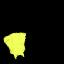
\includegraphics[width=1.8cm, height=1.8cm]{plots/goal.jpg}};

    % Observation inputs & Embeddings (Y = 3) - Labels outside!
    \node[slim, fill=purple!30, label={above:$\boldsymbol{e}^x_{1...t}$}] at (-5.7, 2.5) (ex_box) {};
    \node[funnel, left=0.2cm of ex_box, fill=gray!30] (cnnx) {CNN};
    \node[square, left=0.2cm of cnnx, fill=purple!30, label={below:$\boldsymbol{x}_{1...t}$}] (x_box) {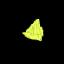
\includegraphics[width=1.8cm, height=1.8cm]{plots/input.jpg}};


    % ================== BIG GC-RSSM & Z BLOCKS ==================
    \begin{scope}[on background layer]
        % Group block surrounding zhat and ztilde - NOW TRANSPARENT
        \node[draw=purple!50, thick, fill=none, rounded corners=5pt, fit=(zhat) (ztilde), inner sep=0.2cm] (zgroup) {};

        % Coordinates to ensure the box pads well around the outer routing loops
        \coordinate (box_bottom) at (0, -1);
        \coordinate (box_left) at (-4.0, 0); 
        \node[draw=gray!80, ultra thick, dashed, fill=none, rounded corners=10pt, fit=(priormlp) (postmlp) (zgroup) (actmlp) (gcrssm) (h) (jointmlp) (box_bottom) (box_left), inner sep=0.42cm] (gcrssm_box) {};
        \node[above left, font=\bfseries, xshift=2.1cm, yshift=0cm, text=gray!80] at (ztilde.east) {GC-RSSM};
    \end{scope}


    % ================== OUTPUTS (FAR RIGHT SIDE) ==================
    % Decoders
    \node[mlpblock, fill=blue!40] at (4.3, 4) (decmlp) {MLP};
    \node[dec_funnel, fill=blue!40] at (4.3, 0) (deccnn) {CNN};

    % Reward Loss (Stacked on top of each other)
    \node[flat, minimum width=1.5cm, fill=blue!40] at (6.3, 4) (rhat) {$\boldsymbol{\hat{r}}_{1...T}$};
    \node[flat, minimum width=1.5cm, fill=blue!40] at (6.3, 5.5) (rgt) {$\boldsymbol{r}_{1...T}$}; 

    % Image Loss (Stacked on top of each other with labels on top and bottom)
    \node[square, label={below:$\boldsymbol{\hat{y}}_{1...T}$}, fill=blue!40] at (6.3, 0) (yhat) {
\includegraphics[width=1.8cm, height=1.8cm]{plots/recon.jpg}};
    \node[square, label={left:$\boldsymbol{y}_{1...T}$}, fill=blue!40] at (6.3, 2.5) (ygt) {
\includegraphics[width=1.8cm, height=1.8cm]{plots/output.jpg}};


    % ================== DATASET & AUGMENTATION (BOTTOM FAR LEFT) ==================
    % 1. Two side-by-side squares positioned below the x_box
    \node[square, below=1.4cm of x_box, xshift=0.6cm,label={below:$\boldsymbol{x}_\text{org}$}] (x_org) {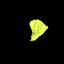
\includegraphics[width=1.8cm, height=1.8cm]{plots/original_obs.jpg}};
    \node[square, right=0.2cm of x_org,label={below:$\boldsymbol{g}_\text{org}$}] (goal_org) {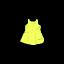
\includegraphics[width=1.8cm, height=1.8cm]{plots/original_goal.jpg}};

    % 2. The Dataset bounding box surrounding the two images
    \node[draw=gray!80, ultra thick, dashed, rounded corners=8pt, fit=(x_org) (goal_org), inner sep=0.4cm] (dataset_box) {};

    % 3. Arrow routing from the far left of the Dataset box to the far left of x_box
    \draw[->, ultra thick, dashed, black, rounded corners] (dataset_box.west) -- ++(-0.6, 0) |- node[pos=0.25, right, align=left, font=\footnotesize\bfseries] {Data Augmentation\\ (training only)} (x_box.west);

    \draw[->, ultra thick, dashed, black, rounded corners] (dataset_box.west) -- ++(-0.6, 0) |-  (g_box.west);
    
    % ================== ROUTING (Clean, 90-Degree Orthogonal) ==================

    % 1. Embeddings to Latent MLPs
    % Slightly offset vertical connection points to avoid line intersection
    \draw[->, ultra thick, red] ([yshift=0.2cm]eg_box.east) -- ([yshift=0.2cm]priormlp.west);
    \draw[->, ultra thick, dashed, orange] ([yshift=0.3cm]ex_box.east) -- ([yshift=-0.2cm]postmlp.west);
    
    % Goal embedding routes down cleanly into the Posterior MLP
    \draw[->, ultra thick, dashed, orange, rounded corners] (eg_box.east) -- ++(0.6,0) |- ([yshift=0.2cm]postmlp.west);

    % 2. MLPs to Latent States & KL Divergence (With Bell Curves!)
    \draw[->, ultra thick, red] (priormlp.east) -- node[above, yshift=2pt] {\tikz[scale=0.3]{\draw[thick] (-1.2,0) -- (1.2,0); \draw[thick, fill=red!80] (-1,0) .. controls (-0.5,0) and (-0.3,1.5) .. (0,1.5) .. controls (0.3,1.5) and (0.5,0) .. (1,0);}} (ztilde.west);
    
    \draw[->, ultra thick, dashed, orange] (postmlp.east) -- node[above, yshift=2pt] {\tikz[scale=0.3]{\draw[thick] (-1.2,0) -- (1.2,0); \draw[thick, fill=orange!40] (-1,0) .. controls (-0.5,0) and (-0.3,1.5) .. (0,1.5) .. controls (0.3,1.5) and (0.5,0) .. (1,0);}} (zhat.west);
    
    \draw[<->, ultra thick, purple, dashed] (ztilde.south) -- node[font=\bfseries] {KL Balance} (zhat.north);

    % 3. h feedback to Latent MLPs
    \draw[->, ultra thick, dashed, orange] (h.north) -- (postmlp.south);
    
    % Route h beautifully to the LEFT of the posterior mlp to reach priormlp
    \draw[->, ultra thick, red, rounded corners] (h.west) -- ++(-0.6, 0) |- ([yshift=-0.2cm]priormlp.west);

    % 4. Action & zhat into Action MLP
    \draw[->, ultra thick, solid, black] (zhat.south) -- (actmlp.north);
    
    % Action sneaks cleanly through a horizontal channel (crosses h-loop at a clean 90 degrees)
    \draw[->, ultra thick, black, rounded corners] (action.east) -- (actmlp.west);

    % 5. Action MLP output into GRU
    \draw[->, ultra thick, black] (actmlp.south) -- (gcrssm.north);

    % 6. GRU output to h, and h recurrent feedback
    \draw[->, ultra thick, black] (gcrssm.west) -- (h.east);
    % Feedback neatly loops left and underneath the GRU
    \draw[->, ultra thick, black, rounded corners] (h.south) -- ++(0,-0.55) -| (gcrssm.south);

    % 7. zgroup & h into Decoding Joint MLP
    % the new bounding box swoops beautifully to the right
    \draw[->, ultra thick, blue, rounded corners] (zgroup.east) -| (jointmlp.north);
    % h swoops beautifully completely under the GRU loop
    \draw[->, ultra thick, blue, rounded corners] ([xshift=-0.2cm]h.south) -- ++(0,-1.0) -| (jointmlp.south);

    % 8. Joint MLP to Decoders (Creates a neat rightward fork)
    \draw[->, ultra thick, blue, rounded corners] (jointmlp.east) -- ++(0.6,0) |- (decmlp.west);
    \draw[->, ultra thick, blue, rounded corners] (jointmlp.east) -- (deccnn.west);

    % 9. Decoders to Final Outputs and Losses (Arrows from decoders removed)
    % Vertical MSE loss arrow directly pointing from predicted to ground truth R
    \draw[<->, ultra thick, dashed, purple] (rhat.north) -- node[right, font=\bfseries] {MSE} (rgt.south);

    % Vertical MSE loss arrow directly pointing from predicted to ground truth Y
    \draw[<->, ultra thick, dashed, purple] (yhat.north) -- node[right, font=\bfseries] {MSE} (ygt.south);
}
        \caption{\addinfo{Network Architecture and Training}}
        \label{fig:network}
    \end{subfigure}
    % --- Main Overarching Caption ---
    \caption{\addinfo{LaGarNet. Figure (a) details the theoretical probabilistic graphical model, whilst (b) presents the network architecture used for its implementation. Matching colours, line styles, blocks, and nodes between both figures signify identical processes. Let $\bm{g}$ denote the goal observation. Throughout both panels, $\bm{x}_t$ and $\bm{z}_t$ represent the observation and latent state before action $\bm{a}_t$, and $\bm{h}_t$ denotes the hidden states of the recurrent backbone. In (a), purple observation nodes and grey action nodes represent known model inputs, whereas yellow action nodes indicate actions sampled during the planning process. In (b), the network integrates observation embeddings (purple) and goal embeddings (green) to learn goal-directed dynamics. A Gated Recurrent Unit (GRU, dark grey) updates the central deterministic belief state, $\boldsymbol{h}$, driven by past actions processed via an MLP (dark grey). The latent state space comprises two distinct mechanisms: the \textit{Prior} network (red blocks, solid pathways) predicts the forward state $\boldsymbol{\tilde{z}}$ conditioned solely on $\boldsymbol{h}$ and $\boldsymbol{g}$, whilst the \textit{Posterior} network (orange blocks, dashed pathways) infers state $\boldsymbol{\hat{z}}$ by integrating the current observation $\boldsymbol{x}$. A balanced KL divergence loss regularises these distributions. Finally, a joint decoder (blue blocks and pathways) maps the combined deterministic and posterior latent states to reconstruct the observation $\boldsymbol{\hat{y}}$ (blue) and predict the expected reward $\boldsymbol{\hat{r}}$ (blue), both optimised using Mean Squared Error (MSE) losses.}}
    \label{fig:lagarnet}
\end{figure*}

\addinfo{Our \text{LaGarNet} method for garment flattening is an offline model-based deep reinforcement learning approach. We train LaGarNet with simulation data using domain randomisation (see Figure \ref{fig:sim-train-init}). We transfer it to the real world for evaluation on the real garments presented in Figure \ref{fig:real-garments} in a zero-shot setting. We achieve generalisation on garment flattening through training a goal-conditioned recurrent state-space model (see Section \ref{sec:gc-rssm} and \ref{sec:architecture}) on a coverage-alignment reward function designed for all garment-flattening tasks (see Section \ref{sec:ca-reward}). We collect simulation data with a more unified data collection procedure  (Section \ref{sec:data-collection}) that uses task-specific Diffusion Policies \ref{sec:diffusion} as a proximal expert policy to collect trajectories around successful distribution. Then, we use a set of data augmentation techniques (see Section \ref{sec:data-aug}) during the training to enable our all-garment LaGarNet achieve state-of-the-art flattening performance with only 100 thousand interactions steps.}

\subsection{Inspiration from Cognitive Psychology}
\addIncrementalg{When presented with a task, humans actively prime their working memory resources to achieve it. To facilitate this, they reconfigure their internal models based on the task's specific features and its current state. Throughout execution, humans maintain task-relevant internal representations to drive inference, generate predictions, and integrate updates as new sensory information arrives. They also utilise these representations of states and transitions to plan towards a desired state. By leveraging these internal models, individuals deduce hidden states from incomplete observations, enabling them to assemble a robust belief state for decision-making under uncertainty and to predict future occurrences. Ultimately, this mechanism allows humans to maintain an inferred estimate of an evolving, sometimes unseen environment, rather than merely reacting to immediate stimuli \cite{miller2001integrative}. In this work, we emulate this working memory process through a Goal-Conditioned Recurrent State Space Model, which processes inputs via an image encoder-decoder framework. Additionally, we incorporate a reward predictor to represent inference and to evaluate how proposed actions impact the task's goal state \cite{hafner2019learning}. Together, this pipeline constitutes our LaGarNet architecture.}

% \subsection{PlaNet-ClothPick} \label{sec:planet-clothpick}

% Building upon general purpose \text{Deep Planning Network (PlaNet)} \cite{hafner2019learning}, \text{PlaNet-ClothPick}  trains a latent dynamic recurrent state-space model (RSSM) in an offline manner on simulated trajectory datasets collected with a particular blend of policies. To incorporate a wide range of manipulation scenarios, the original \text{PlaNet-ClothPick} collects approximately 1 million transition steps to train its recurrent state-space model \cite{hafner2019learning} in an offline manner. Starting from both crumpled and flattened initial states, these steps are generated using a combination of oracle expert, noisy expert, corner-biased, and completely random policies. 

% \text{PlaNet-ClothPick} extends the original \text{Model Predictive Control} planning with a cloth-mask restriction for ensuring the sampled pick actions are within the cloth boundaries on the image space. The planning algorithms utilises the reward prediction from the RSSM to iteratively refine the 1-step action candidates sampled from  Gaussian distributions updated from last iteration's elite candidates. In addition, \text{PlaNet-ClothPick} employs a specific reward function based on difference of Normalised Coverage (NC) between the current and last states, which also encourages the high coverage and penalises misgrasping, overly large action steps and messing up a nearly flattened fabric. 



\subsection{Goal-Conditioned Recurrent State Space Model} \label{sec:gc-rssm}


\addinfo{Our method LaGarNet builds on the mathematical model of State-Space Models (SSMs) that} primarily function as generative frameworks for sequential data, supporting tasks such as inferring future states and learning representations \cite{ma2024interpretable}. Hafner et al. \cite{hafner2019learning} define the Recurrent State-Space Model (RSSM), using a recurrent neural network, under the Partially Observable Markov Decision Process (POMDP) formulation with the following latent state dynamics:
\begin{equation}
\begin{aligned}
    \text{Recurrent dynamic model:} & \quad \bm{h}_t=f(\bm{h}_{t-1},\bm{z}_{t-1},\bm{a}_{t-1}) \\
    \text{Representation model:}    & \quad \hat{\bm{z}}_t\sim q(\hat{\bm{z}}\;|\;\bm{h}_t,\bm{x}_t) \\
    \text{Transition predictor}    & \quad \tilde{\bm{z}}_t\sim p(\tilde{\bm{z}}\;|\;\bm{h}_{t}),
\end{aligned}
\end{equation}
where $\bm{x}$ represents the observation, $\bm{a}$ represents the action, $\bm{h}$ represents the deterministic latent representation, and ($\hat{\bm{z}}$, $\tilde{\bm{z}}$) represent the posterior and prior stochastic latent states. 

LaGarNet trains a goal-conditioned latent dynamics model by learning a feature presentation $\bm{y}$. Specifically, we extend the RSSM with goal-conditioned inference and generation on the latent states as in Figure~\ref{fig:gc-rssm-pgm}, where the same goal observation $\bm{g}$ is incorporated into the estimation of the stochastic latent representation $\bm{z}$. We define GC-RSSM as:

\begin{align}
    \hat{\bm{z}}_t &\sim q(\hat{\bm{z}} \;|\; \bm{h}_t, \bm{x}_t, \bm{g}) 
    && \text{GC Representation Model} \label{eq:gc-repr} \\
    \tilde{\bm{z}}_t &\sim p(\tilde{\bm{z}} \;|\; \bm{h}_t, \bm{g}) 
    && \text{GC Transition Predictor} \label{eq:gc-trans}
\end{align}


\begin{table*}[t]
    \centering
    \caption{\addinfo{Hyperparameters for LaGarNet and Diffusion Policies. GradClip represents gradient clipping. KL denotes Kullback-Leibler divergence, used for latent state regularization. MPC stands for Model Predictive Control, utilised for trajectory planning. EMA refers to Exponential Moving Average, used to stabilise training weights.} \label{tab:all-hyperparameters}}
   
    
    % RIGHT MINIPAGE: Stacked Tables
    \begin{minipage}[t]{0.48\textwidth}
        
        % TOP RIGHT TABLE: Final LaGarNet
        \centering
        \textbf{(a) LaGarNet.} Other parameters are provided in Table (c). \\[0.15cm]
        \begin{tabular}{@{} 
            >{\raggedright\arraybackslash}p{0.50\linewidth} 
            >{\raggedright\arraybackslash}p{0.40\linewidth} @{}}
            \toprule
            \textbf{Hyperparameter} & \textbf{Value} \\
            \midrule
            $\bm{h}, \bm{z}$ Dimensions & 300, 60 \\
            Hidden Dimension & 300 \\
            $\beta_{KL}, \gamma_{KL}, \gamma_{klo}, \gamma_{ro}, \gamma_y, \gamma_r$ & 0.8, 1.0, 0.1, 0.1, 1.0, 1.0 \\
            $\sigma_{min}$, $c$ & 0.1, 1 \\
            $\bm{a}_{\text{no-op}}$ & $\bm{1}$ \\
            MPC Horizon / Candidates/ Iterations & 1 / 5000 / 100 \\
            Backbone Network & GRU RNN \cite{cho2014properties} \\
            \bottomrule
        \end{tabular}
        
        \vspace{0.6cm} % Vertical space between the two stacked tables
        
        % BOTTOM RIGHT TABLE: Final GC-DP
        \textbf{(b) Diffusion Policy for Data Collection.} Other parameters are the same as GC-DP in Table (c).\\[0.15cm]
        \begin{tabular}{@{} 
            >{\raggedright\arraybackslash}p{0.45\linewidth} 
            >{\raggedright\arraybackslash}p{0.45\linewidth} @{}}
            \toprule
            \textbf{Hyperparameter} & \textbf{Value} \\
            \midrule
            Denoising Iterations & 100 \\
            Noise Scheduler & iDDPM \cite{nichol2021improved} \\
            EMA Power \cite{polyak1992acceleration} & 0.75 \\
            Backbone Network & 1D Conditional U-Net \cite{chi2023diffusionpolicy, ronneberger2015u} with disabled Updown \cite{kadi2025draper} \\
            \bottomrule
        \end{tabular}
    \end{minipage}
    \hfill
    \begin{minipage}[t]{0.48\textwidth}
        \centering
        \textbf{(c) Comparison Configurations.}  \\[0.15cm]
        \begin{tabular}{@{} 
            >{\raggedright\arraybackslash}p{0.22\linewidth} 
            >{\raggedright\arraybackslash}p{0.21\linewidth} 
            >{\raggedright\arraybackslash}p{0.21\linewidth} 
            >{\raggedright\arraybackslash}p{0.21\linewidth} @{}}
            \toprule
            \textbf{Hyperparameter} & \textbf{LaGarNet} & \textbf{*-Cmp} & \textbf{GC-DP} \\
            \midrule
            \textbf{$\bm{e}_x$} Dimension & 1024 & 512 & 512 \\
            \textbf{$T_h$} & 49 & 2 & 0 \\
            \textbf{$T_f$} & 1  & 2 & 1 \\
            Sequence Size & 49+1=50 & 2+2=4 & 0+1=1 \\
            Batch Size & 50 & 50 & 64 \\
            Input Resolution & $64 \times 64$ & $64 \times 64$ & $96 \times 96$ \\
            Vision Encoder & PlaNet's CNN \cite{hafner2019learning} & PlaNet's CNN & ResNet-18 \cite{he2016deep} with GroupNorm \cite{wu2018group} \\
            Optimisation & Adam \cite{kingma2015adam} ($\alpha$=$10^{-3}$, $\epsilon$=$10^{-4}$, $\lambda$=0) with GradClip (1000) \cite{pascanu2013difficulty}. & AdamW \cite{loshchilov2019decoupled} ($\alpha$=$10^{-4}$, $\lambda$=$10^{-6}$, $\epsilon$=$10^{-8}$), Cosine Warmup \cite{loshchilov2016sgdr} (500) with GradClip (100)  & AdamW ($\alpha$=$10^{-4}$, $\lambda$=$10^{-6}$, $\epsilon$=$10^{-8}$), Cosine Warmup (500) \\
            \bottomrule
        \end{tabular}
    \end{minipage}%
\end{table*}

The training objective of GC-RSSM is to maximise the marginal log-likelihood of the estimated features and rewards given the sequence of actions and the target goal observation, i.e.,
\begin{equation}
    \argmax_{\theta} \ln p(\bm{y}_{1:T}, r_{1:T} | \bm{a}_{1:T}, \bm{g}). \label{eqn:obj}
\end{equation}

By treating this as Variational Inference and optimising the Evidence Lower Bound (ELBO), we define the generative joint distribution and the approximate posterior from the probabilistic graphical model as:
\begin{align}
    &p(\bm{y}_{1:T}, r_{1:T}, \bm{z}_{1:T} | \bm{a}_{1:T}, \bm{g}) \nonumber \\
    &\quad = \prod_{t=1}^T p(\bm{y}_t|\bm{z}_t) p(r_t|\bm{z}_t) p(\bm{z}_t|\bm{z}_{t-1}, \bm{a}_{t-1}, \bm{g}) \label{eqn:rep-1}\\
    &q(\bm{z}_{1:T}| \bm{x}_{1:T}, \bm{a}_{1:T-1}, \bm{g}) = \prod_{t=1}^T q(\bm{z}_t| \bm{x}_{1:t}, \bm{a}_{1:t-1}, \bm{g}) \label{eqn:rep-2},
\end{align}
where we abstract the deterministic latent states $\bm{h}_t$ as they are directly computed from previous states. Expanding the objective in Equation \ref{eqn:obj} using the distributions in Equations \ref{eqn:rep-1} and \ref{eqn:rep-2}, we obtain the loss function (i.e., the evidence lower bound) of the GC-RSSM as:
\begin{align}
    \mathcal{L} =& \sum_{t=1}^{T} \mathbb{E}_{q(\bm{z}_{1:t-1})} \Bigg[ - 
     \underset{\bm{z}_t \sim q}{\E} \Big[ \ln p(\bm{y}_t|\bm{z}_t) + \ln p(r_t|\bm{z}_t) \Big] \nonumber\\
    &+ \text{KL}\Big[ q(\bm{z}_t|\bm{x}_{1:t}, \bm{a}_{1:{t-1}}, \bm{g}) \;\Big|\Big|\; p(\bm{z}_{t}|\bm{z}_{t-1}, \bm{a}_{t-1}, \bm{g}) \Big]
     \Bigg] \label{eqn:planet-objective-1}.
\end{align}

\addinfo{In practice, for our vision-based application, the goal image $\bm{g} \in \mathbb{R}^{C\times H\times W}$ is processed by the same convolutional encoder as the current observation to produce the goal embedding $\bm{e}_g$. To allow backpropagation through the stochastic latent states during training, we sample the latent state $\bm{z}$ from the estimated Gaussian distributions using the reparameterisation trick \cite{kingma2013auto}:
\begin{equation}
    \bm{z} = \bm{\mu} + \bm{\sigma} \odot \bm{\epsilon}, \quad \text{where } \bm{\epsilon} \sim \mathcal{N}(\bm{0}, \bm{I}) \label{eqn:reparam}
\end{equation}
In order to ensure a strictly positive standard deviation $\bm{\sigma}$ and prevent numerical collapse, the raw network output for the variance is processed through a softplus activation function, i.e., $f(x)=\ln(1+e^x)$ in addition to a minimum threshold $\sigma_{min}$ \cite{glorot2011deep}.}

\addinfo{Optimising the overall objective requires carefully balancing its various loss terms using scalar coefficients. We use MSE loss (as it is equivalent to negative log-likelihood under Gaussian Distribution \cite{goodfellow2016deep}) for the feature and reward prediction, and they are weighted by scales $\gamma_x$ and $\gamma_r$ in the final loss function (see Equation \ref{eqn:total-loss}), respectively. For the latent regularisation, we adopt the KL balancing technique \cite{hafner2021mastering} to scale the gradients differently for the prior and posterior networks, ensuring the prior moves toward the posterior faster than vice versa. Furthermore, to prevent posterior collapse---where the latent variables fail to encode useful information---we apply a ``free nat'' minimum threshold, $c$, clipping the penalty when the divergence falls below this value (e.g., 1 nat) \cite{hafner2019learning}. The balanced KL divergence loss is formally defined as:
\begin{equation}
\begin{aligned}
    \mathcal{L}_{KL} = &\beta_{KL} \max\Big(c, \text{KL}\big[\text{sg}(q(\hat{\bm{z}}_t)) \;\big|\big|\; p(\tilde{\bm{z}}_t)\big]\Big) \\ 
    &+ (1 - \beta_{KL}) \max\Big(c, \text{KL}\big[q(\hat{\bm{z}}_t) \;\big|\big|\; \text{sg}(p(\tilde{\bm{z}}_t))\big]\Big)
\end{aligned} \label{eqn:kl-balance}
\end{equation}
where $\text{sg}(\cdot)$ denotes the stop-gradient operator \cite{hafner2025mastering}, and the entire term is scaled by the coefficient $\gamma_{KL}$ in the final total loss function. Finally, to enforce consistent multi-step future predictions, we compute overshooting losses (i.e. calculation based on more than one-step priors) for the KL divergence and reward predictions of future prior latent states across $T_f$ steps, weighted by $\gamma_{klo}$ and $\gamma_{ro}$, respectively in the final total loss function (Equation \ref{eqn:total-loss}). Please refer to Table \ref{tab:all-hyperparameters} for the exact coefficient values adopted for LaGarNet.}

During training, we do not stop any gradients on the goals, but we stop them for overshooting loss. We use GC-RSSM to avoid recurrent structure of the model from ``forgetting'' information of the goal. \addinfo{Combining all the aforementioned components, we formally express the total loss function as:
\begin{equation}
    \mathcal{L}_{total} = \gamma_y \mathcal{L}_y + \gamma_r \mathcal{L}_r + \gamma_{KL} \mathcal{L}_{KL} + \gamma_{klo} \mathcal{L}_{klo} + \gamma_{ro} \mathcal{L}_{ro} \label{eqn:total-loss}
\end{equation}
where $\mathcal{L}_y$ and $\mathcal{L}_r$ denote the MSE losses for feature and reward estimation, whilst $\mathcal{L}_{klo}$ and $\mathcal{L}_{ro}$ represent the corresponding overshooting losses computed over $T_f$ steps. For more detailed architecture information and hyperparameters for training, please see Section \ref{sec:architecture} and Table \ref{tab:all-hyperparameters}}.

\addinfo{At test time, LaGarNet takes the current and goal observations, $(\bm{x}_t, \bm{g})$. It maintains the posterior latent states $(\bm{h}_t, \hat{\bm{z}}_t)$ by updating them with the previous action $\bm{a}_{t-1}$ and the current observation. Initially, the latent state vectors are set to zero. The model obtains the initial posterior latent states by applying a no-operation action, $\bm{a}_{\text{no-op}}$, to these zero-initialised states, yielding:
\begin{equation}
    (\hat{\bm{z}}_0, \bm{h}_1) \sim \Big(q(\hat{\bm{z}}_0 \;|\; \bm{0}, \bm{x}_1, \bm{g}), f(\bm{0}, \hat{\bm{z}}_{0}, \bm{a}_{\text{no-op}})\Big).
\end{equation}
Next, it selects the first action $\bm{a}_t$ from a planned sequence of length $T_f$ using the Cross-Entropy Method for Model Predictive Control (MPC-CEM), formulated as:
\begin{align}
   \bm{a}_{t:t+T_f-1} = \argmax_{\bm{a}} \sum_{k=t}^{t+T_f-1} r_\theta(\tilde{\bm{z}}_{k+1}(\bm{a}_k)),
\end{align}
where $\tilde{\bm{z}}_{k+1}(\bm{a}_k) \sim p(\tilde{\bm{z}}_{k+1} \;|\; \bm{h}_{k+1}=f(\bm{h}_k, \hat{\bm{z}}_k, \bm{a}_k), \bm{g})$. In our garment flattening setup, we set the prior future prediction horizon to $T_f=1$. }

% Furthermore, we modify the MPC-CEM to restrict pick actions to the cloth mask, consistent with \text{PlaNet-ClothPick}, and adapt the planning to accommodate changing workspace constraints, as detailed in Algorithm \ref{alg:mpc-cem-single-act}.}
% In your preamble:
% \usepackage[linesnumbered, ruled, vlined]{algorithm2e}

% \begin{algorithm}[t]
% \caption{\addinfo{Object Mask Pick-and-Place MPC-CEM}}
% \label{alg:mpc-cem-single-act}

% % This command enables line numbers for this specific algorithm block
% % if you didn't enable it globally in the preamble.
% \LinesNumbered 

% \KwIn{
%   (1) Binary masks for object $\mathcal{M}_{\text{obj}}$ and workspace $\mathcal{M}_{\text{ws}} \in \{0,1\}^{H \times W}$ \\
%   (2) Predictive trajectory cost function $J$ \\
%   (3) Action space boundaries $a_{\text{min}}, a_{\text{max}} \in \mathbb{R}^A$ \\
%   (4) CEM hyperparameters: iterations $K$, population size $N$, elite count $N_{e}$
% }
% \KwOut{Optimised action $a^* \in \mathbb{R}^A$}

% \BlankLine
% $\mu \leftarrow \mathbf{0}^A$, $\sigma \leftarrow \mathbf{1}^A$ \;
% $\mathcal{M}_{\text{pk}} = \mathcal{M}_{\text{obj}} \cap \mathcal{M}_{\text{ws}}$ \;

% \BlankLine
% \For{$i = 1 \dots K$}{
%     $\mathcal{S} \leftarrow \{a_j\}_{j=1}^N \sim \mathcal{N}(\mu, \operatorname{diag}(\sigma^2))$ \;
    
%     \BlankLine
%     $\mathcal{S}_{\text{valid}} \leftarrow \left\{ a \in \mathcal{S} \mid p = \text{norm2pixel}(a), \, \mathcal{M}_{\text{pk}}(p_{:2}) \wedge \mathcal{M}_{\text{ws}}(p_{2:4}) \right\}$\;
%     $\mathcal{S}_{\text{valid}} \leftarrow \text{clip}(\mathcal{S}_{\text{valid}}, a_{\text{min}}, a_{\text{max}})$ \;
    
%     \BlankLine
%     $\mathcal{S}_{\text{elite}} \leftarrow \operatorname*{arg\,min}_{\mathcal{S}' \subset \mathcal{S}_{\text{valid}}, |\mathcal{S}'|=N_e} \sum_{a \in \mathcal{S}'} J(a)$ \;
    
%     \BlankLine
%     $\mu \leftarrow \frac{1}{N_e} \sum_{a \in \mathcal{S}_{\text{elite}}} a$ \;
%     $\sigma \leftarrow \sqrt{\frac{1}{N_e} \sum_{a \in \mathcal{S}_{\text{elite}}} (a - \mu)^2}$ \;
% }
% \BlankLine
% \Return{$\text{clip}(\mu, a_{\text{min}}, a_{\text{max}})$}
% \end{algorithm}
\addinfo{\subsection{LaGarNet's Network Architecture} \label{sec:architecture}}

\addinfo{As shown in Figure \ref{fig:network}, our method LaGarNet consists of four primary components: an image encoder, an image decoder, a goal-conditioned transition model, and a reward predictor. All hidden layers of the neural networks utilise ReLU activation functions \cite{fukushima1975cognitron}.}

\subsubsection{Image Encoder \& Decoder} \addinfo{The visual encoder processes the $64 \times 64$ RGB images (either the current observation $\bm{x}_t$ or the goal observation $\bm{g}$) into a 1024-dimensional continuous embedding, denoted as $\bm{e}_t$ and $\bm{e}_g$ respectively. The network comprises four sequential convolutional blocks. For the $64 \times 64$ resolution, the blocks have channel sizes of $\{32, 64, 128, 256\}$. Each block utilises a kernel size of $4 \times 4$ and a stride of $2$. The output of the final convolutional layer is flattened and projected via a linear layer to match the designated embedding dimension.}

\addinfo{The observation decoder acts as a generative model $p(\hat{\bm{x}}_t \;|\; \bm{h}_t, \bm{z}_t)$ to reconstruct the mask image from the latent space, which is primarily used to compute the observation reconstruction loss. It takes the concatenated deterministic state $\bm{h}_t$ and stochastic state $\bm{z}_t$ (sampled from the posterior $\hat{\bm{z}}_t$ during training) as input, processes it through a linear dense layer, and reshapes it into a $1 \times 1$ spatial feature map. This is followed by four transposed convolutional layers with channel sizes of $\{128, 64, 32, C\}$, where $C$ is the number of channels in the output observation. The first two transposed convolutions use a kernel size of $5 \times 5$, whilst the final two use a kernel size of $6 \times 6$, all with a stride of $2$.}

\subsubsection{Goal-Conditioned Transition Model} \addinfo{The transition dynamics of the GC-RSSM composes of multi-layer perceptrons (MLPs) and a Gated Recurrent Unit (GRU) \cite{cho2014properties}. The recurrent state $\bm{h}_t = f(\bm{h}_{t-1}, \bm{z}_{t-1}, \bm{a}_{t-1})$ is updated using a GRU cell. The input to the GRU is the output of a 1-layer MLP that fuses the previous stochastic latent state $\bm{z}_{t-1}$ and the previous action $\bm{a}_{t-1}$. The prior stochastic state $\tilde{\bm{z}}_t \sim p(\tilde{\bm{z}} \;|\; \bm{h}_t, \bm{g})$ is predicted by concatenating the current deterministic state $\bm{h}_t$ and the goal embedding $\bm{e}_g$. This concatenated vector is passed through an embedding MLP, followed by a state-prior MLP that outputs the mean and variance of a diagonal Gaussian distribution. The standard deviation is parameterised using a Softplus function bounded by a minimum value ($\sigma_{\text{min}} = 0.1$) to prevent numerical instability and mode collapse.}

\addinfo{During training, the posterior stochastic state $\hat{\bm{z}}_t \sim q(\hat{\bm{z}} \;|\; \bm{h}_t, \bm{x}_t, \bm{g})$ incorporates the current observation $\bm{x}_t$. The deterministic state $\bm{h}_t$, goal embedding $\bm{e}_g$, and current observation embedding $\bm{e}_t$ are concatenated and processed through an embedding MLP. A subsequent state-posterior MLP outputs the mean and variance of the posterior diagonal Gaussian distribution, similarly bounded by the Softplus function.}

\subsubsection{Reward Predictor} \addinfo{The reward model $r_\theta(\bm{h}_t, \bm{z}_t)$ predicts the expected scalar reward $r_t$ from the current latent state. It takes the concatenated deterministic state $\bm{h}_t$ and stochastic state $\bm{z}_t$, processes them through four hidden layers and projects them to a scalar value via a final linear layer to formulate a 5-layer MLP.}

\subsection{Coverage-Alignment Reward}  \label{sec:ca-reward}

Our coverage-alignment reward $\mathcal{R}_{CA}$  uses the step-wise \addtypo{normalised} coverage \addtypo{(NC)} difference $\mathcal{R}_{dC}$ \addinfo{and} the difference of maximum intersection-over-union (\text{Max IoU}) between the current and goal cloth mask, denoted as $\mathcal{R}_{du}$. Mathematically, our reward function can be expressed as follows: 

\begin{equation}
    \mathcal{R}_{CA} = \alpha_r \times\mathcal{R}_{dc} + (1-\alpha_r)\times \mathcal{R}_{du},
\end{equation}
\addinfo{where $\mathcal{R}_{dC} = \text{NC}_t - \text{NC}_{t-1}$ and $\mathcal{R}_{du} = \text{MaxIoU}_t - \text{MaxIoU}_{t-1}$; both $\mathcal{R}_{dC}$ and $\mathcal{R}_{du} \in [-1, 1]$ , so that $\mathcal{R}_{CA} \in [-1, 1]$} In our experiments, we set $\alpha_r$ as \addinfo{0.3} for our final LaGarNet. \addinfo{This reward function turns out to be easy to learn due to its continous and linear nature.}

\begin{figure}[t]
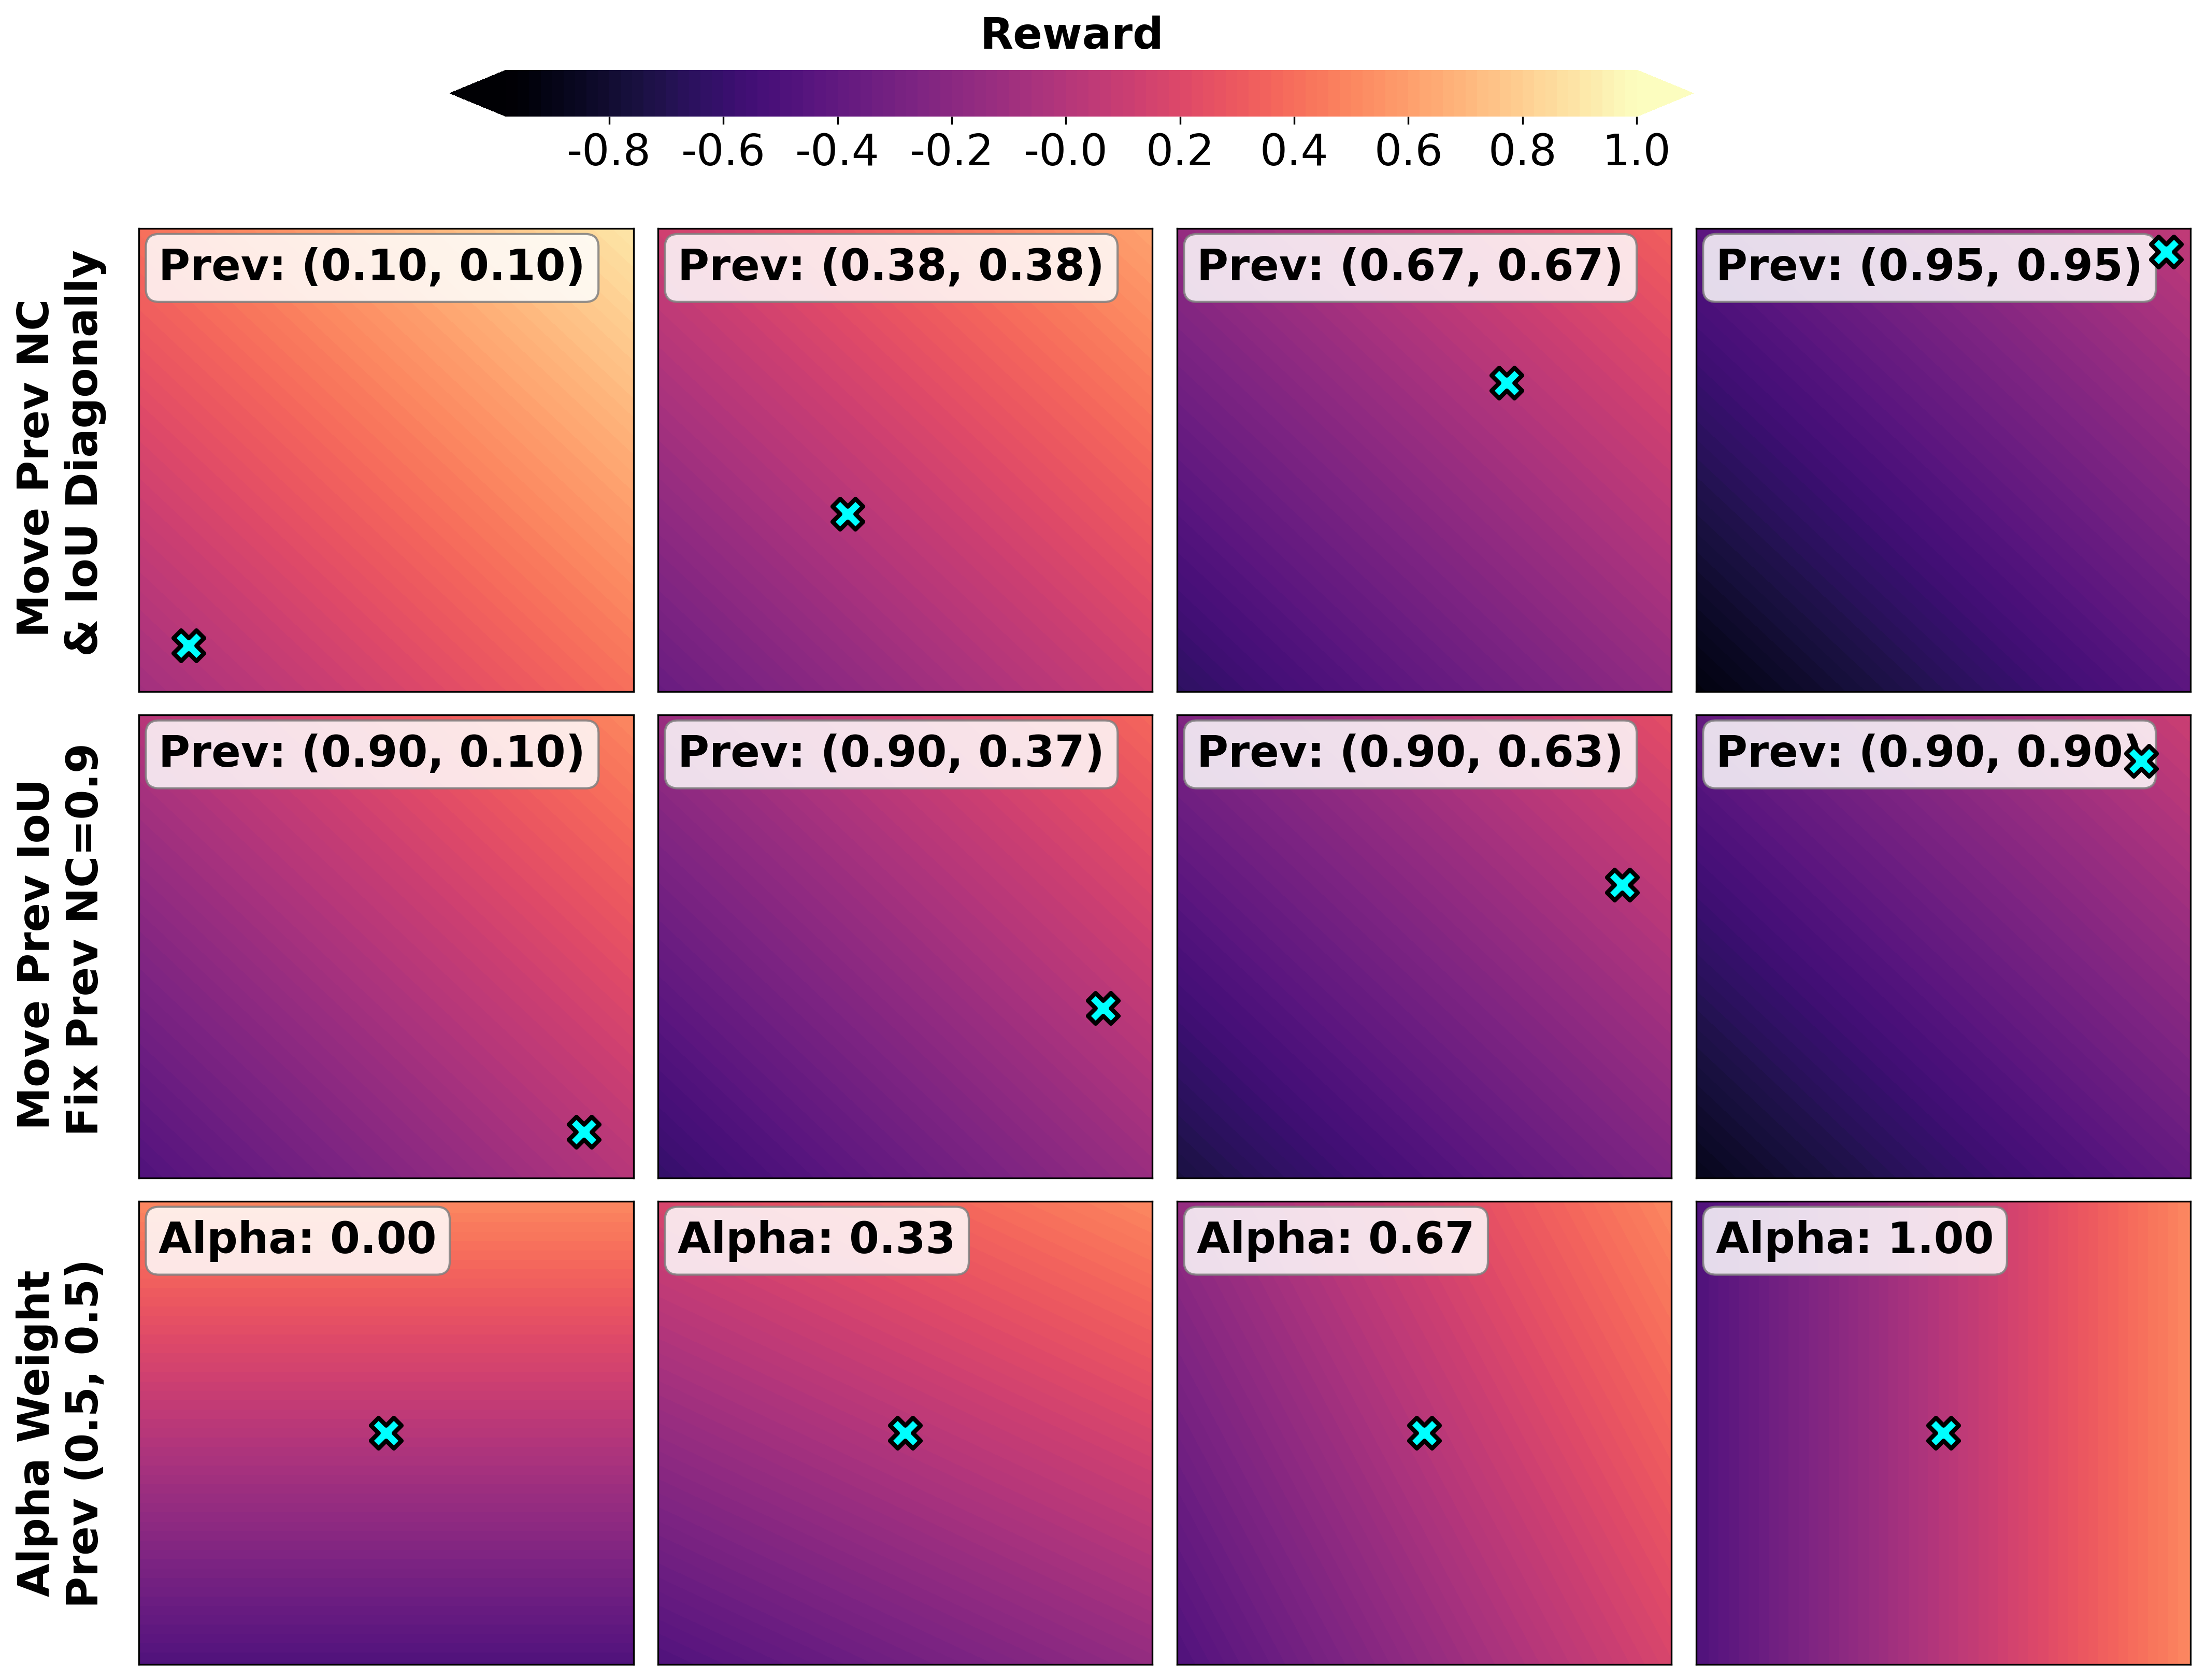
\includegraphics[width=0.48\textwidth]{plots/reward_sensitivity_3x5.png}
    \caption{\addinfo{Coverage Alignment Reward}}
        \label{fig:reward-function}
\end{figure}

% \begin{figure*}[t!]
%     \centering
%     \begin{subfigure}[t]{0.5\linewidth}
% 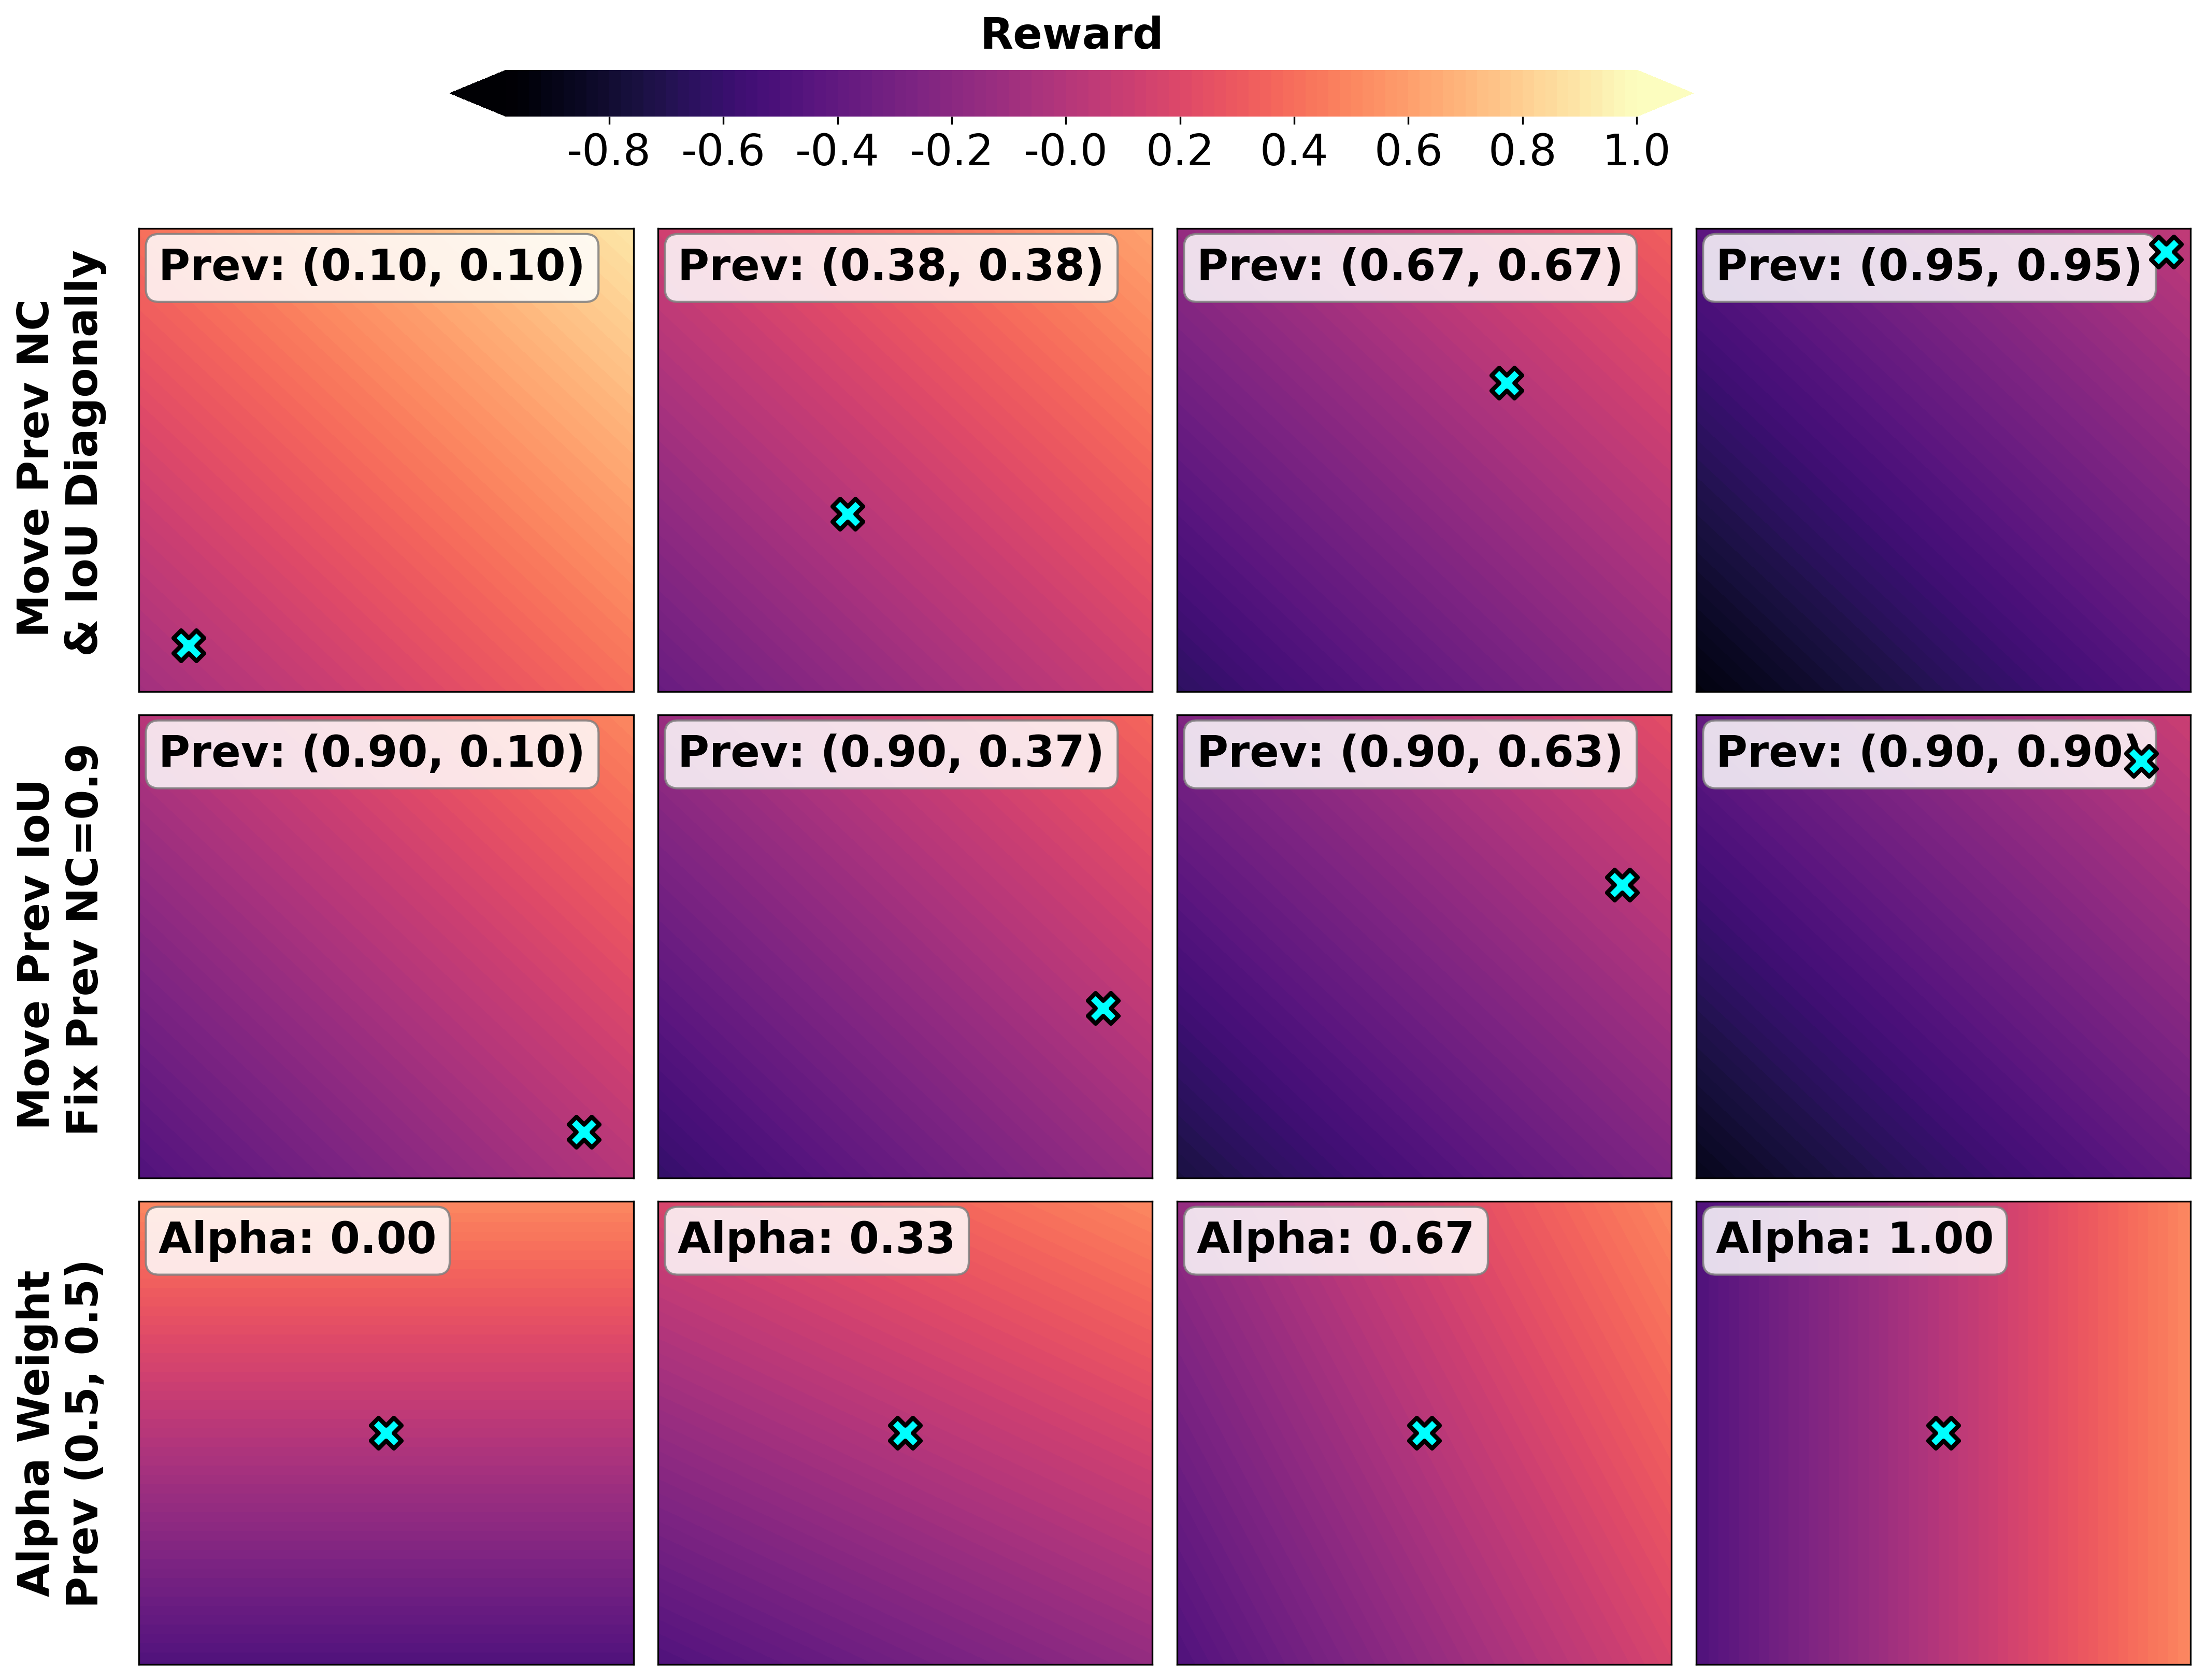
\includegraphics[width=\textwidth]{plots/reward_sensitivity_3x5.png}
%     \caption{\addinfo{Coverage Alignment Reward}}
%         \label{fig:reward-function}
%     \end{subfigure}
%     \hfill
%     \begin{subfigure}[t]{0.44\linewidth}
% 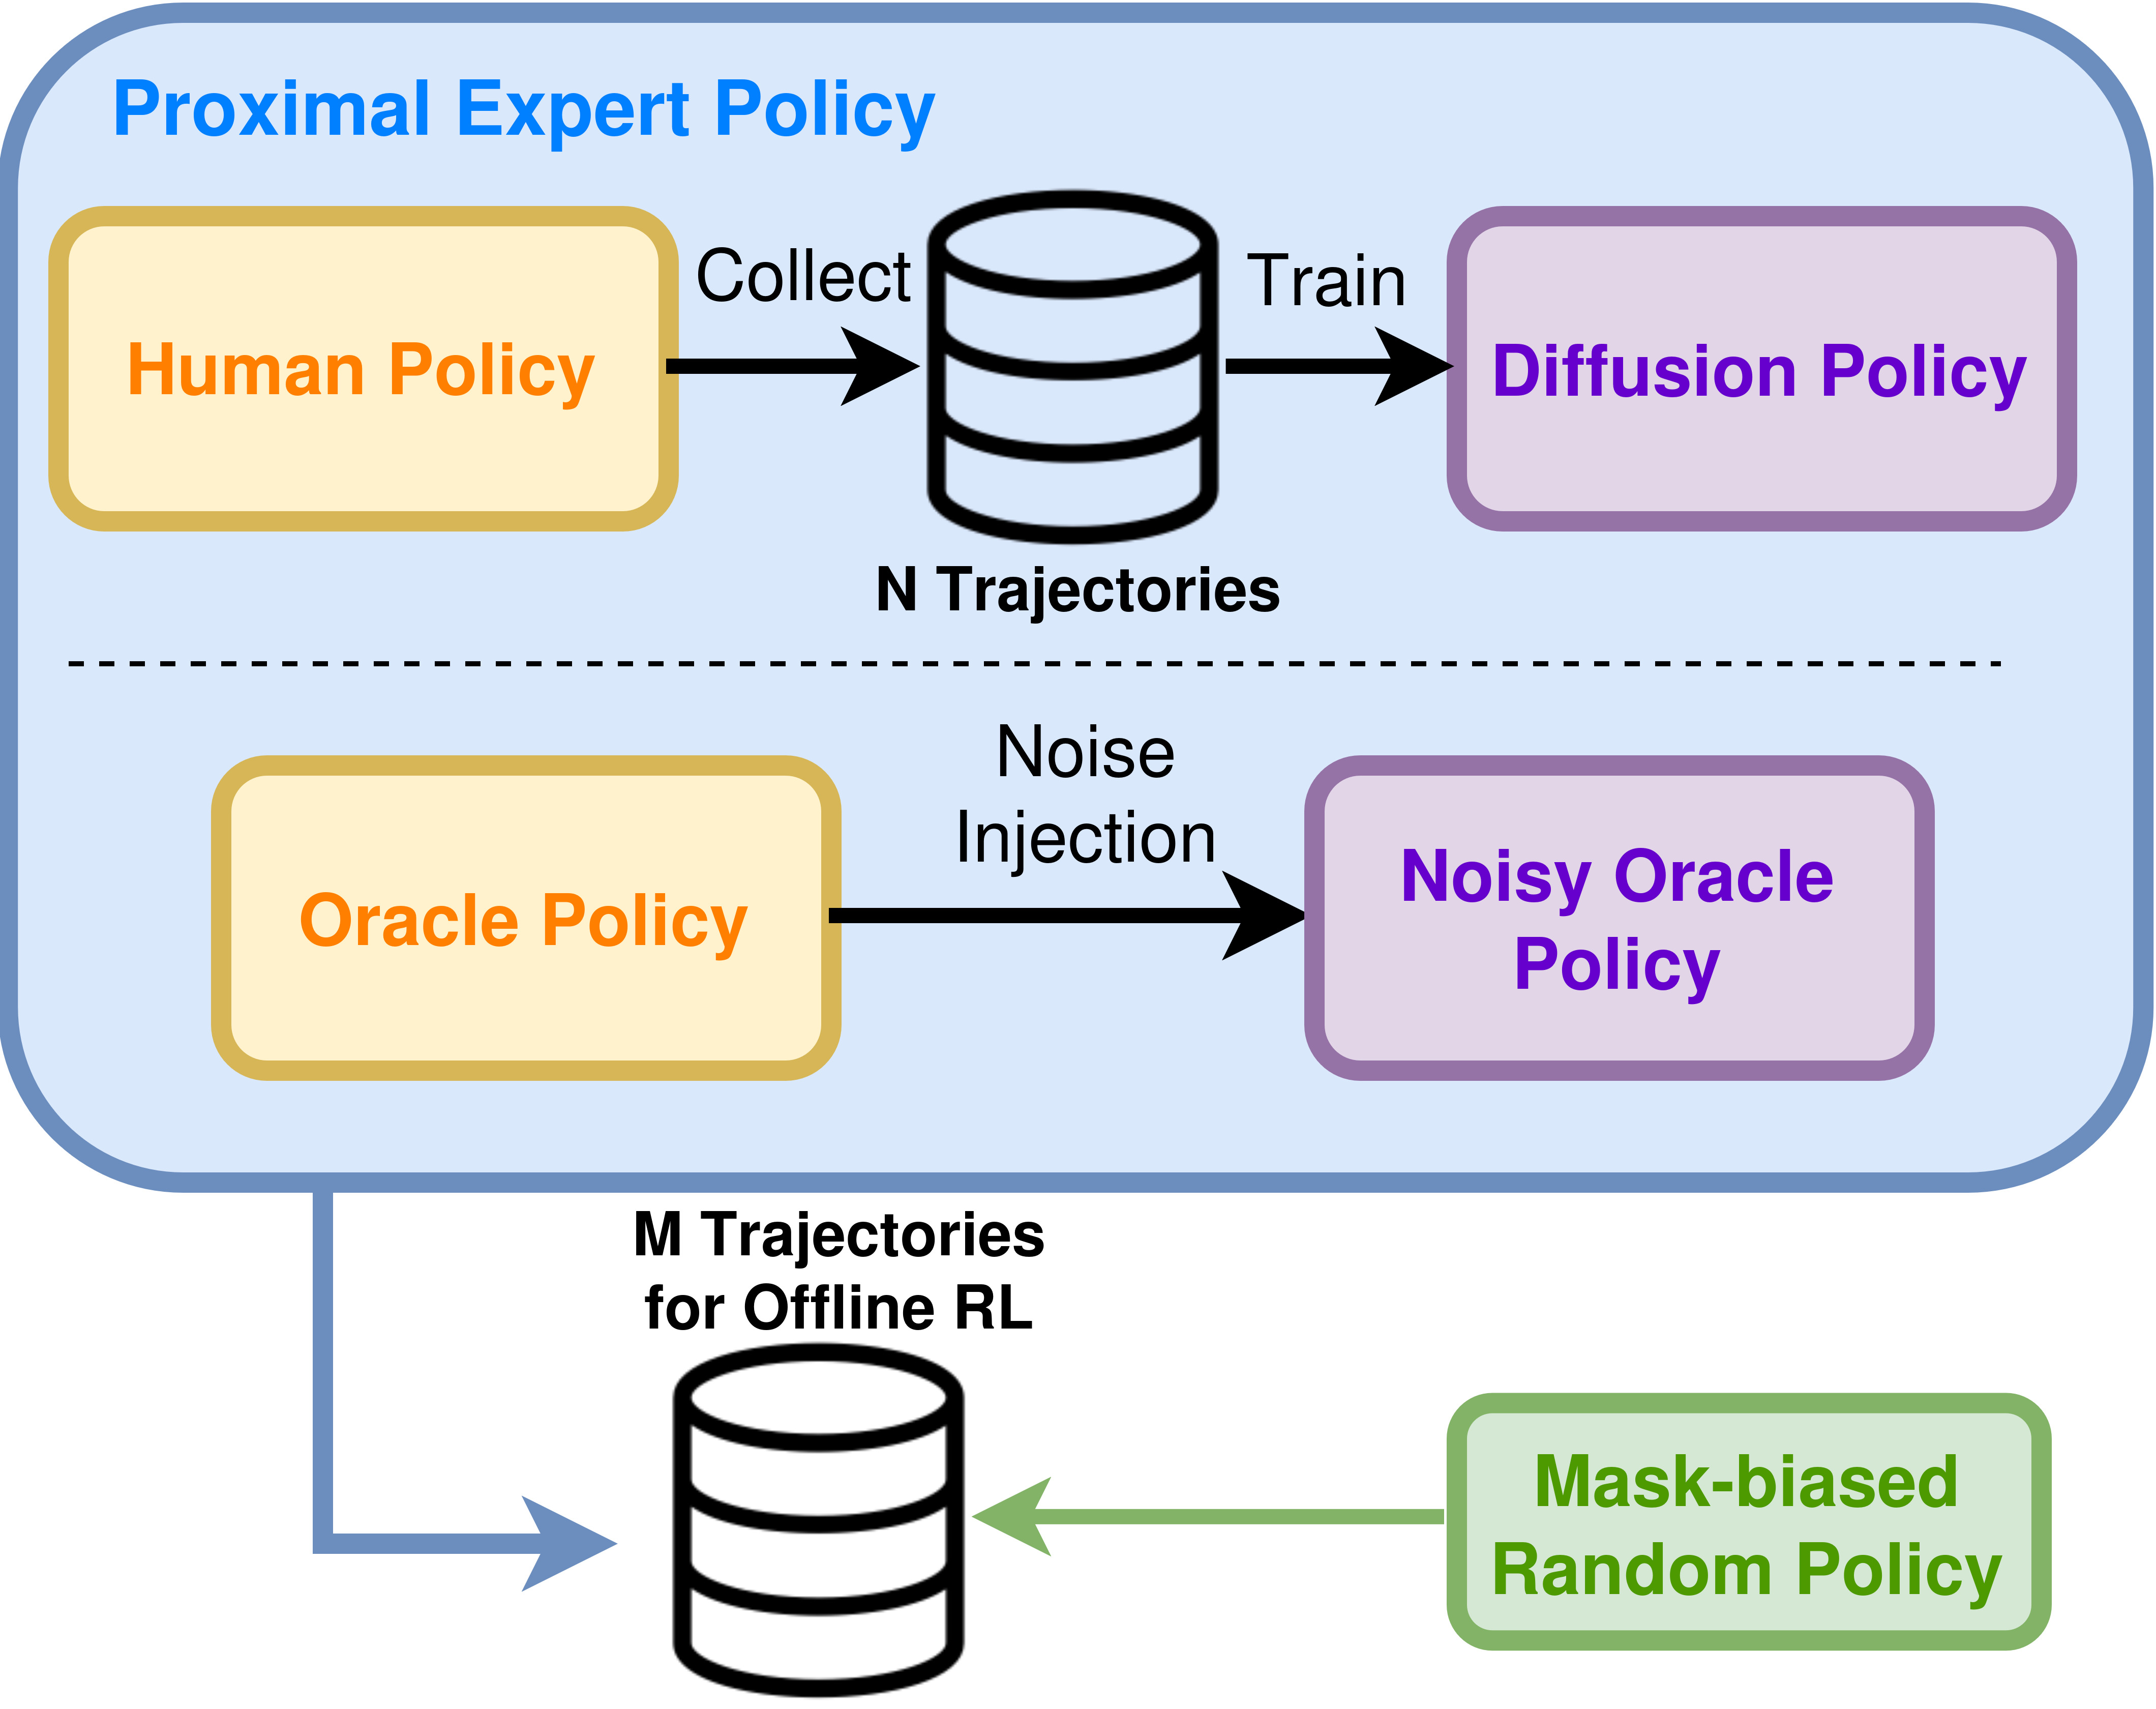
\includegraphics[width=\textwidth]{plots/lagarnet-data-collection.jpg}
%     \caption{\addinfo{Data Collection}}
%         \label{fig:data-collection}
%     \end{subfigure}
%     % --- Main Overarching Caption ---
%     \caption{LaGarNet's Reward and Data Collection Procedure.}
%     \label{fig:lagarnet}
% \end{figure*}
\subsection{Data Collection \addIncrementalg{with Proximal Expert and Random Policies}} \label{sec:data-collection}

Previous RSSM-based cloth flattening models \cite{kadi2024planet} often relied on strong inductive biases stemming from a complex and specific blend of data collection policies. We also find that engineering flattening oracle policies for complex garment types, such as T-shirts and trousers, is an extremely challenging task. This difficulty defeats the simplicity advantage of imitation learning and makes offline reinforcement learning difficult to train, as it prevents the easy collection of trajectories around the successful region of the distribution. Our \text{LaGarNet} method mitigates these biases by employing a  \addIncrementalg{proximal expert policy} and a mask-biased random policy (see Algorithm \ref{alg:data-collection}). 

\begin{algorithm}[t]
\caption{Data Collection with Diffusion and Random Policies for Offline Reinforcement Learning}
\label{alg:data-collection}
\LinesNumbered 
\KwIn{(1) Human/Expert demonstrations $\mathcal{D}_{\text{demo}}$,\\ (2) a random policy $\pi_{rdm}$,\\ (3) number of trajectories $M$ for collection, and \\ (4) ratio $r$ of diffusion trajectories}
\KwOut{Collected dataset $\mathcal{D}$ of trajectories}

\BlankLine

Train a Diffusion Policy $\pi_{\text{diff}}$ on $\mathcal{D}_{\text{demo}}$ \;

\BlankLine
\For{$i = 1$ \KwTo $M$}{
    Sample $u \sim \text{Uniform}(0,1)$ \;
    \eIf{$u < r$}{
        Unroll trajectory $\tau$ using $\pi_{\text{diff}}$ \;
    }{
        Unroll trajectory $\tau$ using $\pi_{rdm}$ \;
    }
    $\mathcal{D}$.add($\tau$) \;
}
\BlankLine
\Return{$\mathcal{D}$}
\end{algorithm}

We train a Diffusion Policy \cite{chi2023diffusionpolicy} (see Section \ref{sec:diffusion}) using a few human demonstrations in the garment domain to replace the rigid oracle expert policies often required by previous methods \cite{kadi2024planet}. \addIncrementalg{The reason we utilise a diffusion policy for garment domains is because a true oracle is exceptionally difficult to develop; furthermore, as shown in Table \ref{tab:longsleeve-flattening}, the Diffusion Policy can induce numerous nearly successful flattening trajectories---its action diversity accounts for some noisiness in manipulation, which can be harnessed to diversify the data distribution around near-successful regions. }

\addinfo{To ensure our exploration strategy aligns seamlessly with the downstream object-masked MPC planner---which inherently restricts pick positions to the cloth mask---we introduce a novel mask-biased random policy. Rather than relying on the completely random or corner-biased policies prevalent in prior works, our approach uniformly samples a pick pixel directly from the object mask and a place pixel from anywhere within the image. By pairing the Diffusion Policy with this mask-biased exploration at a 1:1 ratio, we purposefully curate a rich, targeted dataset and significantly reduce the inductive biases that typically constrain earlier algorithms.}
\addinfo{\subsection{Diffusion Policy for the P\&P Domain} \label{sec:diffusion}}

\addinfo{We adopt the Diffusion Policy~\cite{chi2023diffusionpolicy} to generate proximal expert trajectories for garment flattening for offline RL training. We utilise the policy version adapted for the pick-and-place cloth-manipulation domain given by \textsc{DRAPER}~\cite{kadi2025draper}; it formulates quasi-static pick-and-place cloth manipulation as a conditional generative process. Unlike deterministic regressors, the Diffusion Policy learns a stochastic policy that progressively refines noisy proposals into feasible actions conditioned on visual observations.}

\addinfo{The Diffusion Policy models the conditional distribution of action sequences $\pi(\bm{A}^t \mid \bm{X}^t)$. It defines the action sequence $\bm{A}^t \equiv \{\bm{a}_i\}_{i=t-T_h}^{t+T_f-1}$ over a prediction horizon $T_p = T_h + T_f$, and the observation history $\bm{X}^t \equiv \{\bm{x}_i\}_{i=t-T_h}^{t}$ over a horizon $T_h$. In our pick-and-place setting, $\bm{a}_i \in \mathbb{R}^d$ represents a continuous vector parameterising grasp locations and target placements with $d=4$.
The framework consists of a forward process and a learned reverse process. The forward process incrementally corrupts the clean action sequence $\bm{A}_0$ with Gaussian noise over $K$ steps. The noisy sequence at step $k$ can be sampled directly as:
\begin{equation}
\bm{A}_k \sim \mathcal{N}\big(\sqrt{\bar{\alpha}_k}\bm{A}_0, (1 - \bar{\alpha}_k)\bm{I}\big),
\end{equation}
where $\bar{\alpha}_k$ is derived from a predefined squared-cosine noise schedule $\{\beta_i\}_{i=1}^k$~\cite{nichol2021improved}.
The reverse process generates actions by iteratively denoising a sample from a standard Gaussian prior, $\bm{A}_K \sim \mathcal{N}(\bm{0}, \bm{I})$. A learned noise prediction network $\epsilon_\theta$ (1D U-Net \cite{ronneberger2015u}) takes the noisy action $\bm{A}_k$, the diffusion step $k$, and a conditioning observation embedding $\bm{e}_x$ as inputs to estimate the injected noise; the embedding $\bm{e}_x$ is derived from a vision encoder (ResNet18 \cite{he2016deep} with Group Normalisation \cite{wu2018group}) applied to $\bm{X}$. For garment flattening tasks, we disable temporal convolution in the 1D U-Net noise predictor by setting $T_h = 0$ and $T_f = 1$, as longer context windows have proved disadvantageous in our experiments.}

\addinfo{The refined action sequence for the previous step is computed as:
\begin{equation}
\bm{A}_{k-1} =
\frac{1}{\sqrt{1 - \beta_k}}
\Big(
\bm{A}_k -
\frac{\beta_k}{\sqrt{1 - \bar{\alpha}k}}
\epsilon_\theta(\bm{A}_k, k, \bm{e}_x)
\Big)
+ \sigma_k \boldsymbol{\epsilon},
\end{equation}
where $\boldsymbol{\epsilon} \sim \mathcal{N}(\bm{0}, \bm{I})$ and $\sigma_k$ controls the stochasticity of the sampler.}

\addinfo{Diffusion Policy trains the network to maximise the conditional log-likelihood of the action sequence by minimising the evidence lower bound (ELBO), resulting in the mean squared error (MSE) objective:
\begin{equation}
\mathcal{L} = \mathrm{MSE}\Big(\boldsymbol{\epsilon}_k, \epsilon_\theta(\bm{A}_k, k, \bm{e}_x)\Big).
\label{eqn:diffusion-policy-loss}
\end{equation}}
\addinfo{\subsection{Data Augmentation} \label{sec:data-aug}}

\addinfo{In order to ensure the robust generalisation of our visual policy, we employ a comprehensive, geometry-aware data augmentation pipeline on the current and goal RGB observations.}

\addinfo{The RGB inputs undergo an appearance-level augmentation where they are remapped to a [0, 1] range and injected with subtle Gaussian noise with $\sigma$ of 0.01. Then, we apply rigorous spatial transformations to the current state observations to expand the effective dataset and enforce $SE(2)$ equivariance in the learned policy --- we apply continuous random rotations with 1 degree intervals and vertical flips with a 50\% probability to the current RGB and mask images. Crucially, to maintain geometric consistency, we strictly couple these visual transformations with the action space. When the images are rotated or flipped, the corresponding 2D spatial pixel actions (the pick-and-place coordinates) are transformed via equivalent rotation matrices and coordinate inversions,  discarding any transformations that push the pixel actions out of bounds.}

\addinfo{Finally, to enable robust goal-conditioned behaviour in the real world, the pipeline applies independent affine transformations to the goal RGB observation. These images undergo randomised 2D rigid body transformations, combining rotations and translational shifts (up to a translation scale of 0.2). By independently augmenting the target visual states, we prevent the transformer from simply memorising exact pixel-to-pixel mappings between the current and goal images; it forces the architecture to learn deeper, spatially robust relational features for the pick-and-place task.}

\section{Experiments} \label{sec:experiments}

\addIncrementalg{In this section, we design our experiments to answer the following research questions:}

\addIncrementalg{1) \textbf{Section \ref{sec:comp-sota}:} How does LaGarNet's performance compare to other state-of-the-art (SoTA) baselines for single-picker pick-and-place flattening methods?}

\addIncrementalg{2) \textbf{Section \ref{sec:comp-diff}:} What is the advantage of using the GC-RSSM model in the garment flattening domain compared to a diffusion policy?} 

\addIncrementalg{3) \textbf{Section \ref{sec:abl}:} How important are the different components of LaGarNet?} 

\addIncrementalg{4) \textbf{Section \ref{sec:real-exp}:} How does LaGarNet perform in the real world?}    


\addinfo{To rigorously evaluate the performance of our garment flattening policy, we employ the following standard metrics:}

\addinfo{1) \textbf{Normalised Coverage (NC):} The ratio of the garment's current 2D projected area to its maximally flattened area. This metric isolates the extent of unfolding and is bounded to $[0, 1]$.}

\addinfo{2) \textbf{Normalised Improvement (NI):} The relative increase in coverage from the initial configuration, defined as $\frac{c_t - c_0}{c_{\text{max}} - c_0}$, where $c_t$, $c_0$, and $c_{\text{max}}$ denote the current, initial, and maximally flattened coverage, respectively. }

\addinfo{3) \textbf{Maximum Intersection-over-Union (Max IoU):} The highest IoU overlap between the current garment segmentation mask and the target flattened mask. This evaluates the precise spatial alignment and shape matching of the garment through rotation and translation.}

\addinfo{4) \textbf{Success Rate (SR):} The percentage of trials that reach a terminal state satisfying strict flattening and alignment criteria, empirically defined as achieving both $\text{NC} > 90\%$ and $\text{Max IoU} > 80\%$ in the same state. The SR is defined on 20-step horizon by default, unless it is specificity defined.}

\addinfo{For NC, NI, Max IoU, We report the maximum value achieved from the initial states to a given action step in a trajectory. For both simulated and real-world experiments, the goal state (i.e., the maximally flattened configuration) of each garment must be predefined and captured prior to the execution of the trials to serve as the ground-truth reference for computing the aforementioned metrics---it is also needed as an input to goal-condition policies. In simulation, we use the off-the-shelf generated states by Canberk et al. \cite{canberk2023cloth}, whilst in the real world, we must first set the garment to flattened states then manually put it into crumpled states to start. In both simulation and real-world environment, we ignore the slight discrepancy caused by the relative position between the garment and camera viewpoint and its field of view, as it does not obviously affect either the training or evaluation of these policies in both setups.}
\begin{table}[!t]
\centering
\caption{\addinfo{Simulation Configurations. We need to scale down the garments 0.32 on our longsleeve set so to get the optimal performance for MEDOR.}}
\label{tab:sim-config}
\begin{tabular}{@{}lcc@{}}
\toprule
\textbf{Parameter} & \textbf{Ours} & \textbf{MEDOR's} \\ \midrule
Garment Scale from Cloth3D & 0.8 & 0.32\\
Stiffness (Stretch, Bend, Shear) & (0.75, 0.02, 0.02) & (1.2, 0.6, 1.0) \\
Particle Radius (m) & 0.014 & 0.005 \\
Camera Height (m) & 2 & 0.65\\
FoV (degree) & 45 & 45\\
Mass (kg) & 1 (Total) & $3e^{-3}$ (Per Particle) \\
Dynamic/ Particle Frictions & 0.75 / 1.0&  1.0 / 1.2\\
Damping & 1 & 1 \\
\bottomrule
\end{tabular}
\end{table}

\begin{figure*}[t!]
    \centering
    \begin{subfigure}[t]{0.37\linewidth}
        \vspace{0pt}
        \centering 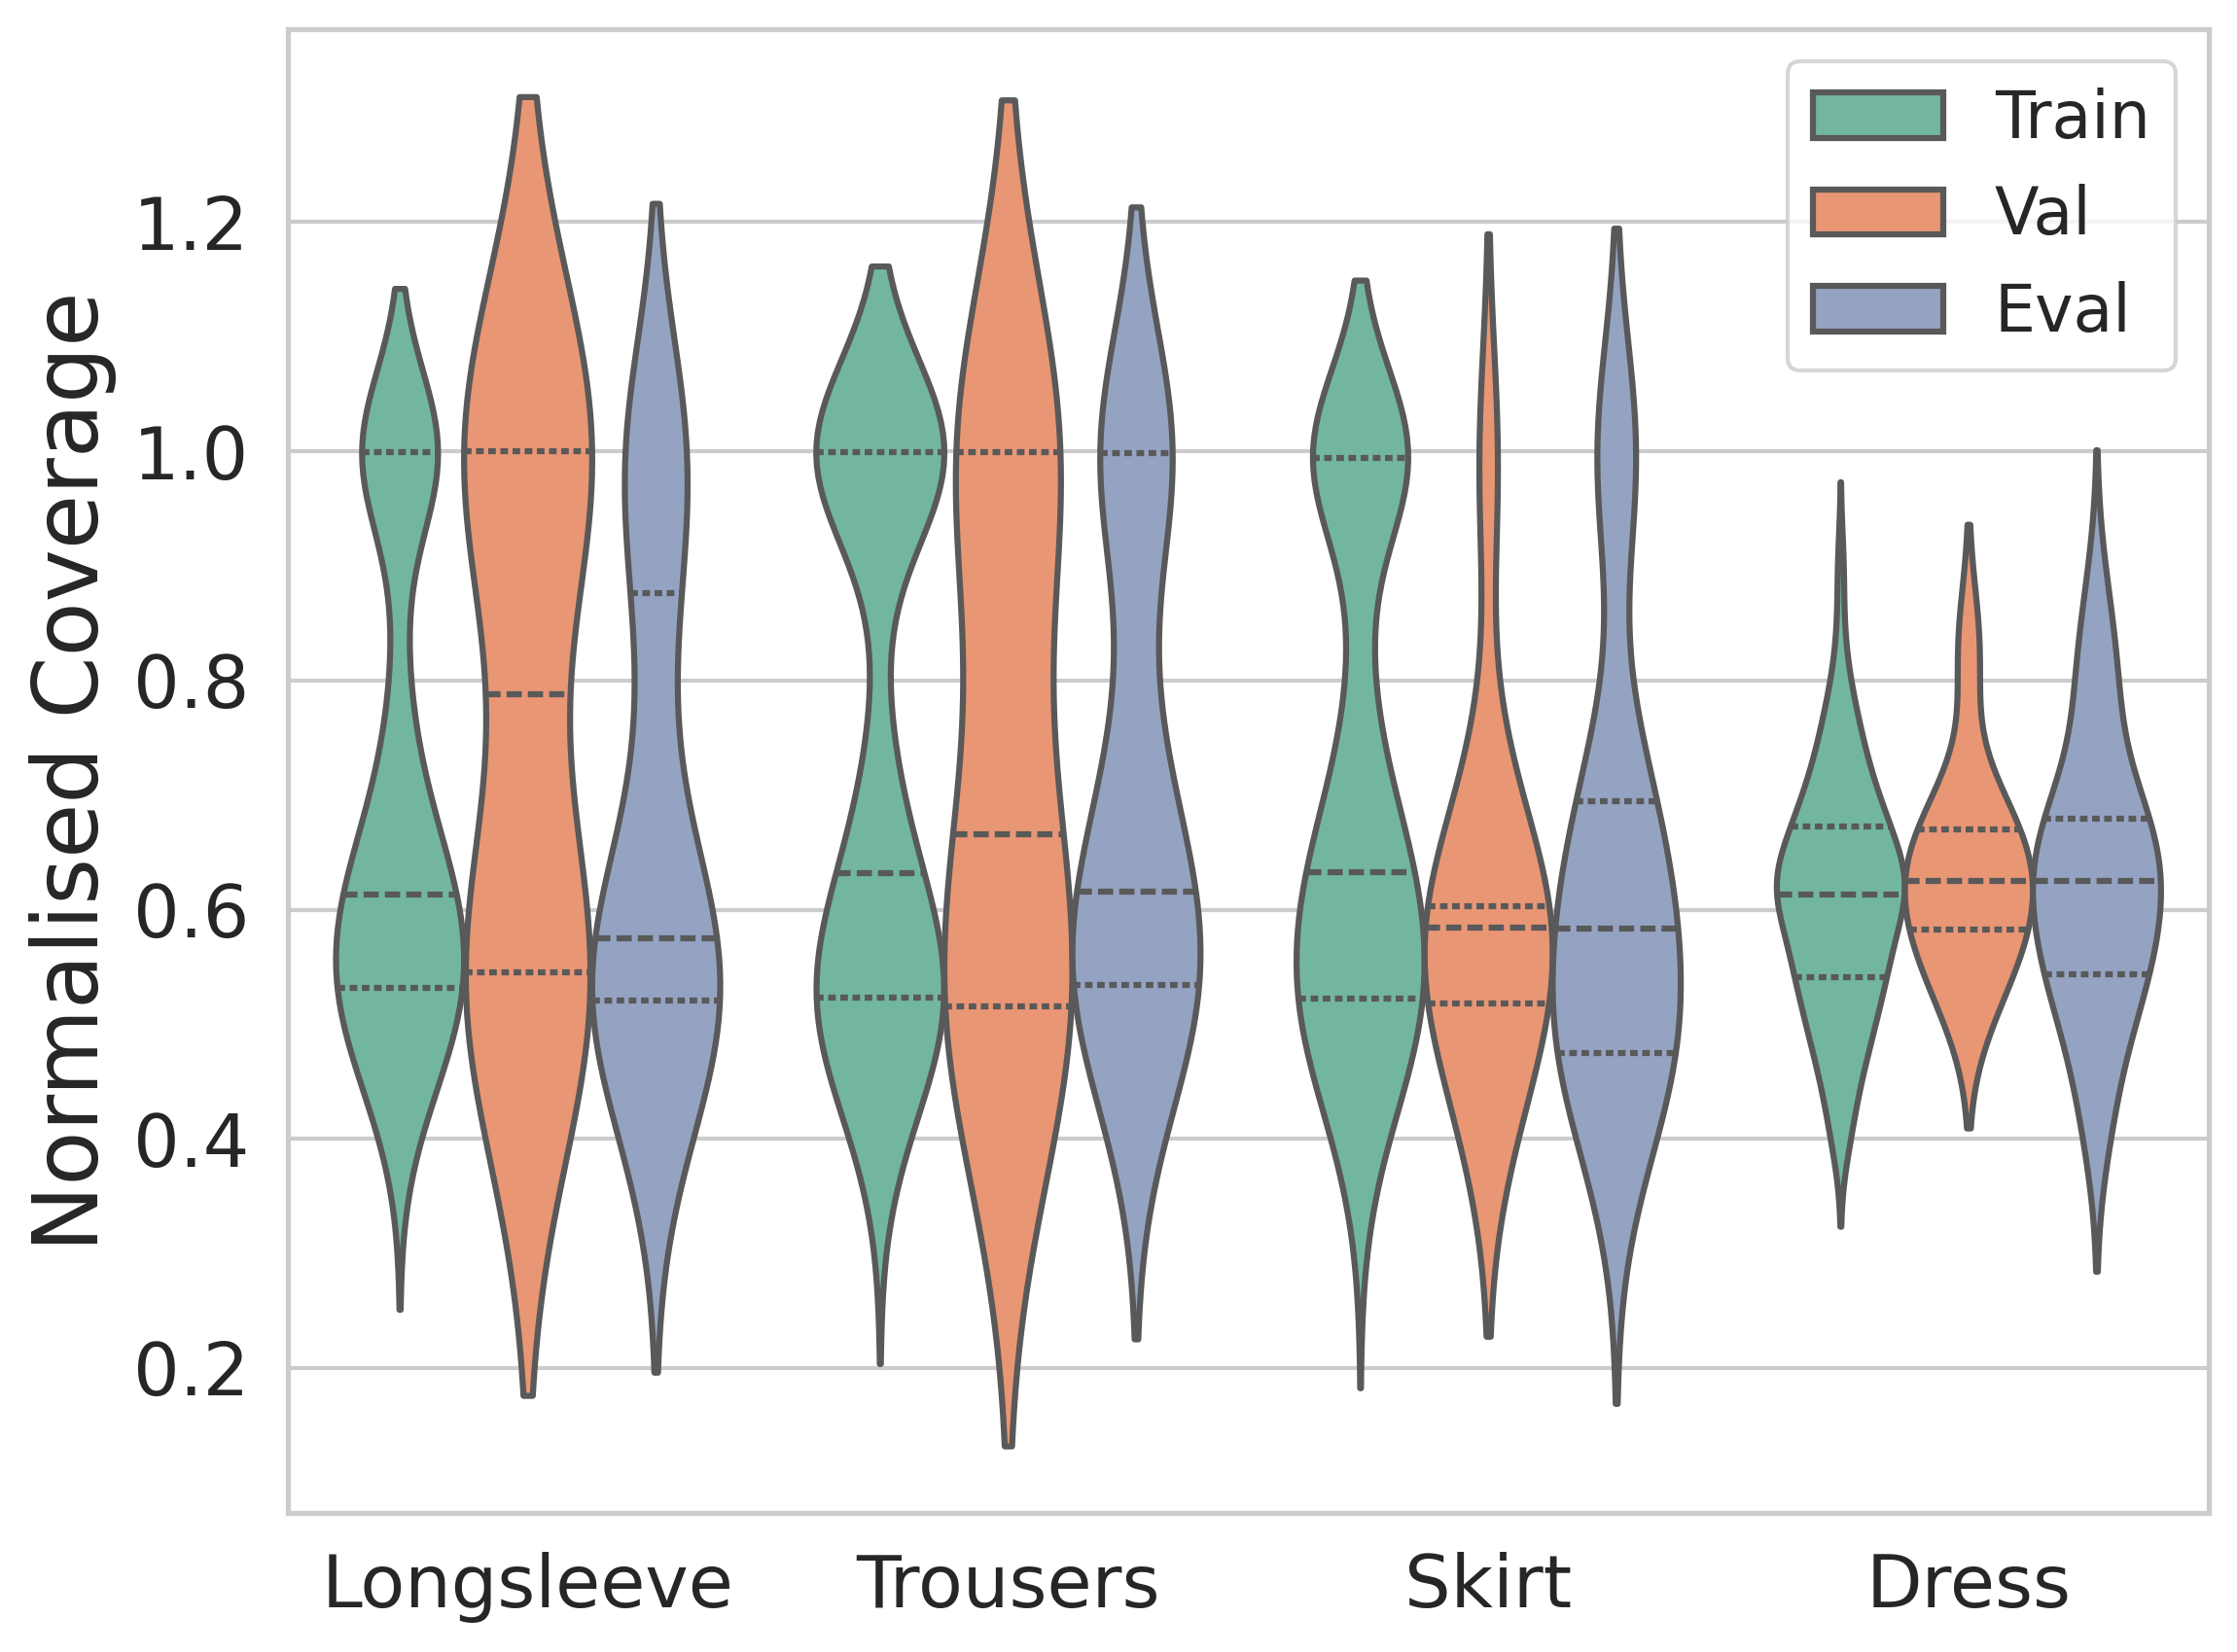
\includegraphics[width=\linewidth]{plots/normalized_coverage_distribution.png}
        \caption{Normalised Coverage Distribution}
        \label{fig:nc-dist}
    \end{subfigure}
    \begin{subfigure}[t]{0.37\linewidth}
        \vspace{0pt}
        \centering 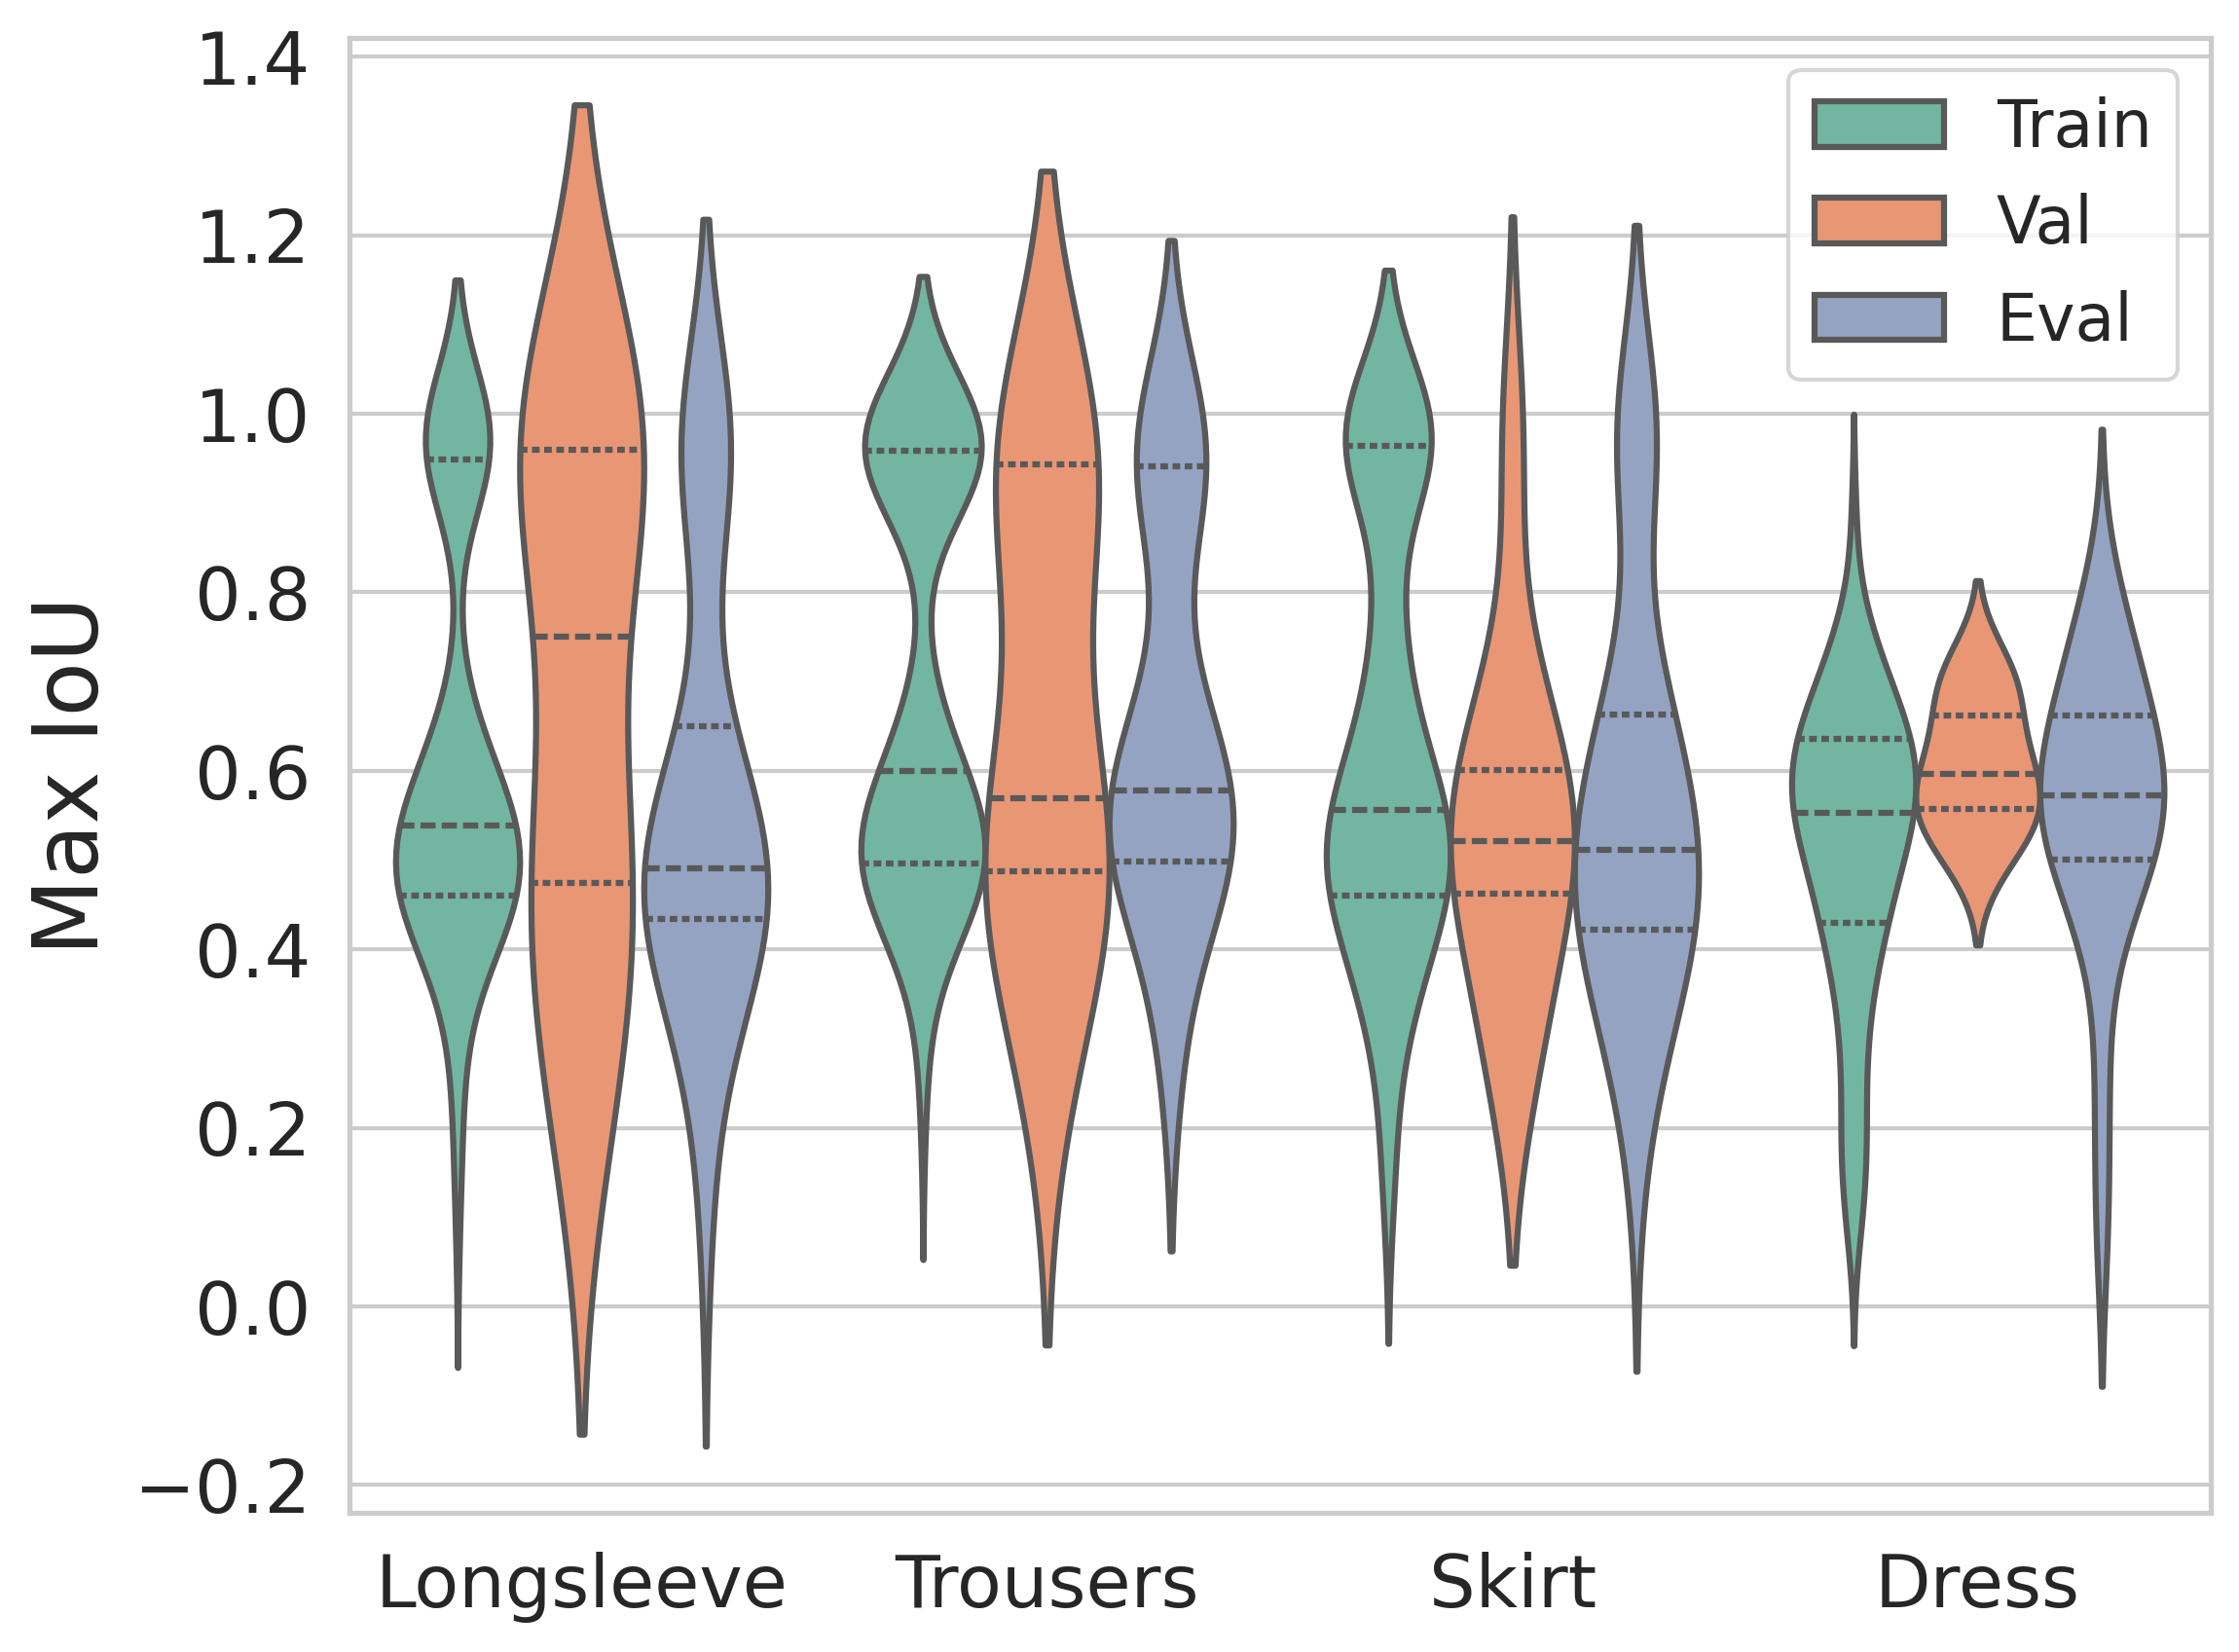
\includegraphics[width=\linewidth]{plots/max_iou_distribution.png}
        \caption{Max IoU Distribution}
        \label{fig:iou-dist}
    \end{subfigure}
    \begin{subfigure}[t]{0.24\linewidth}
        \vspace{0pt}
        \centering 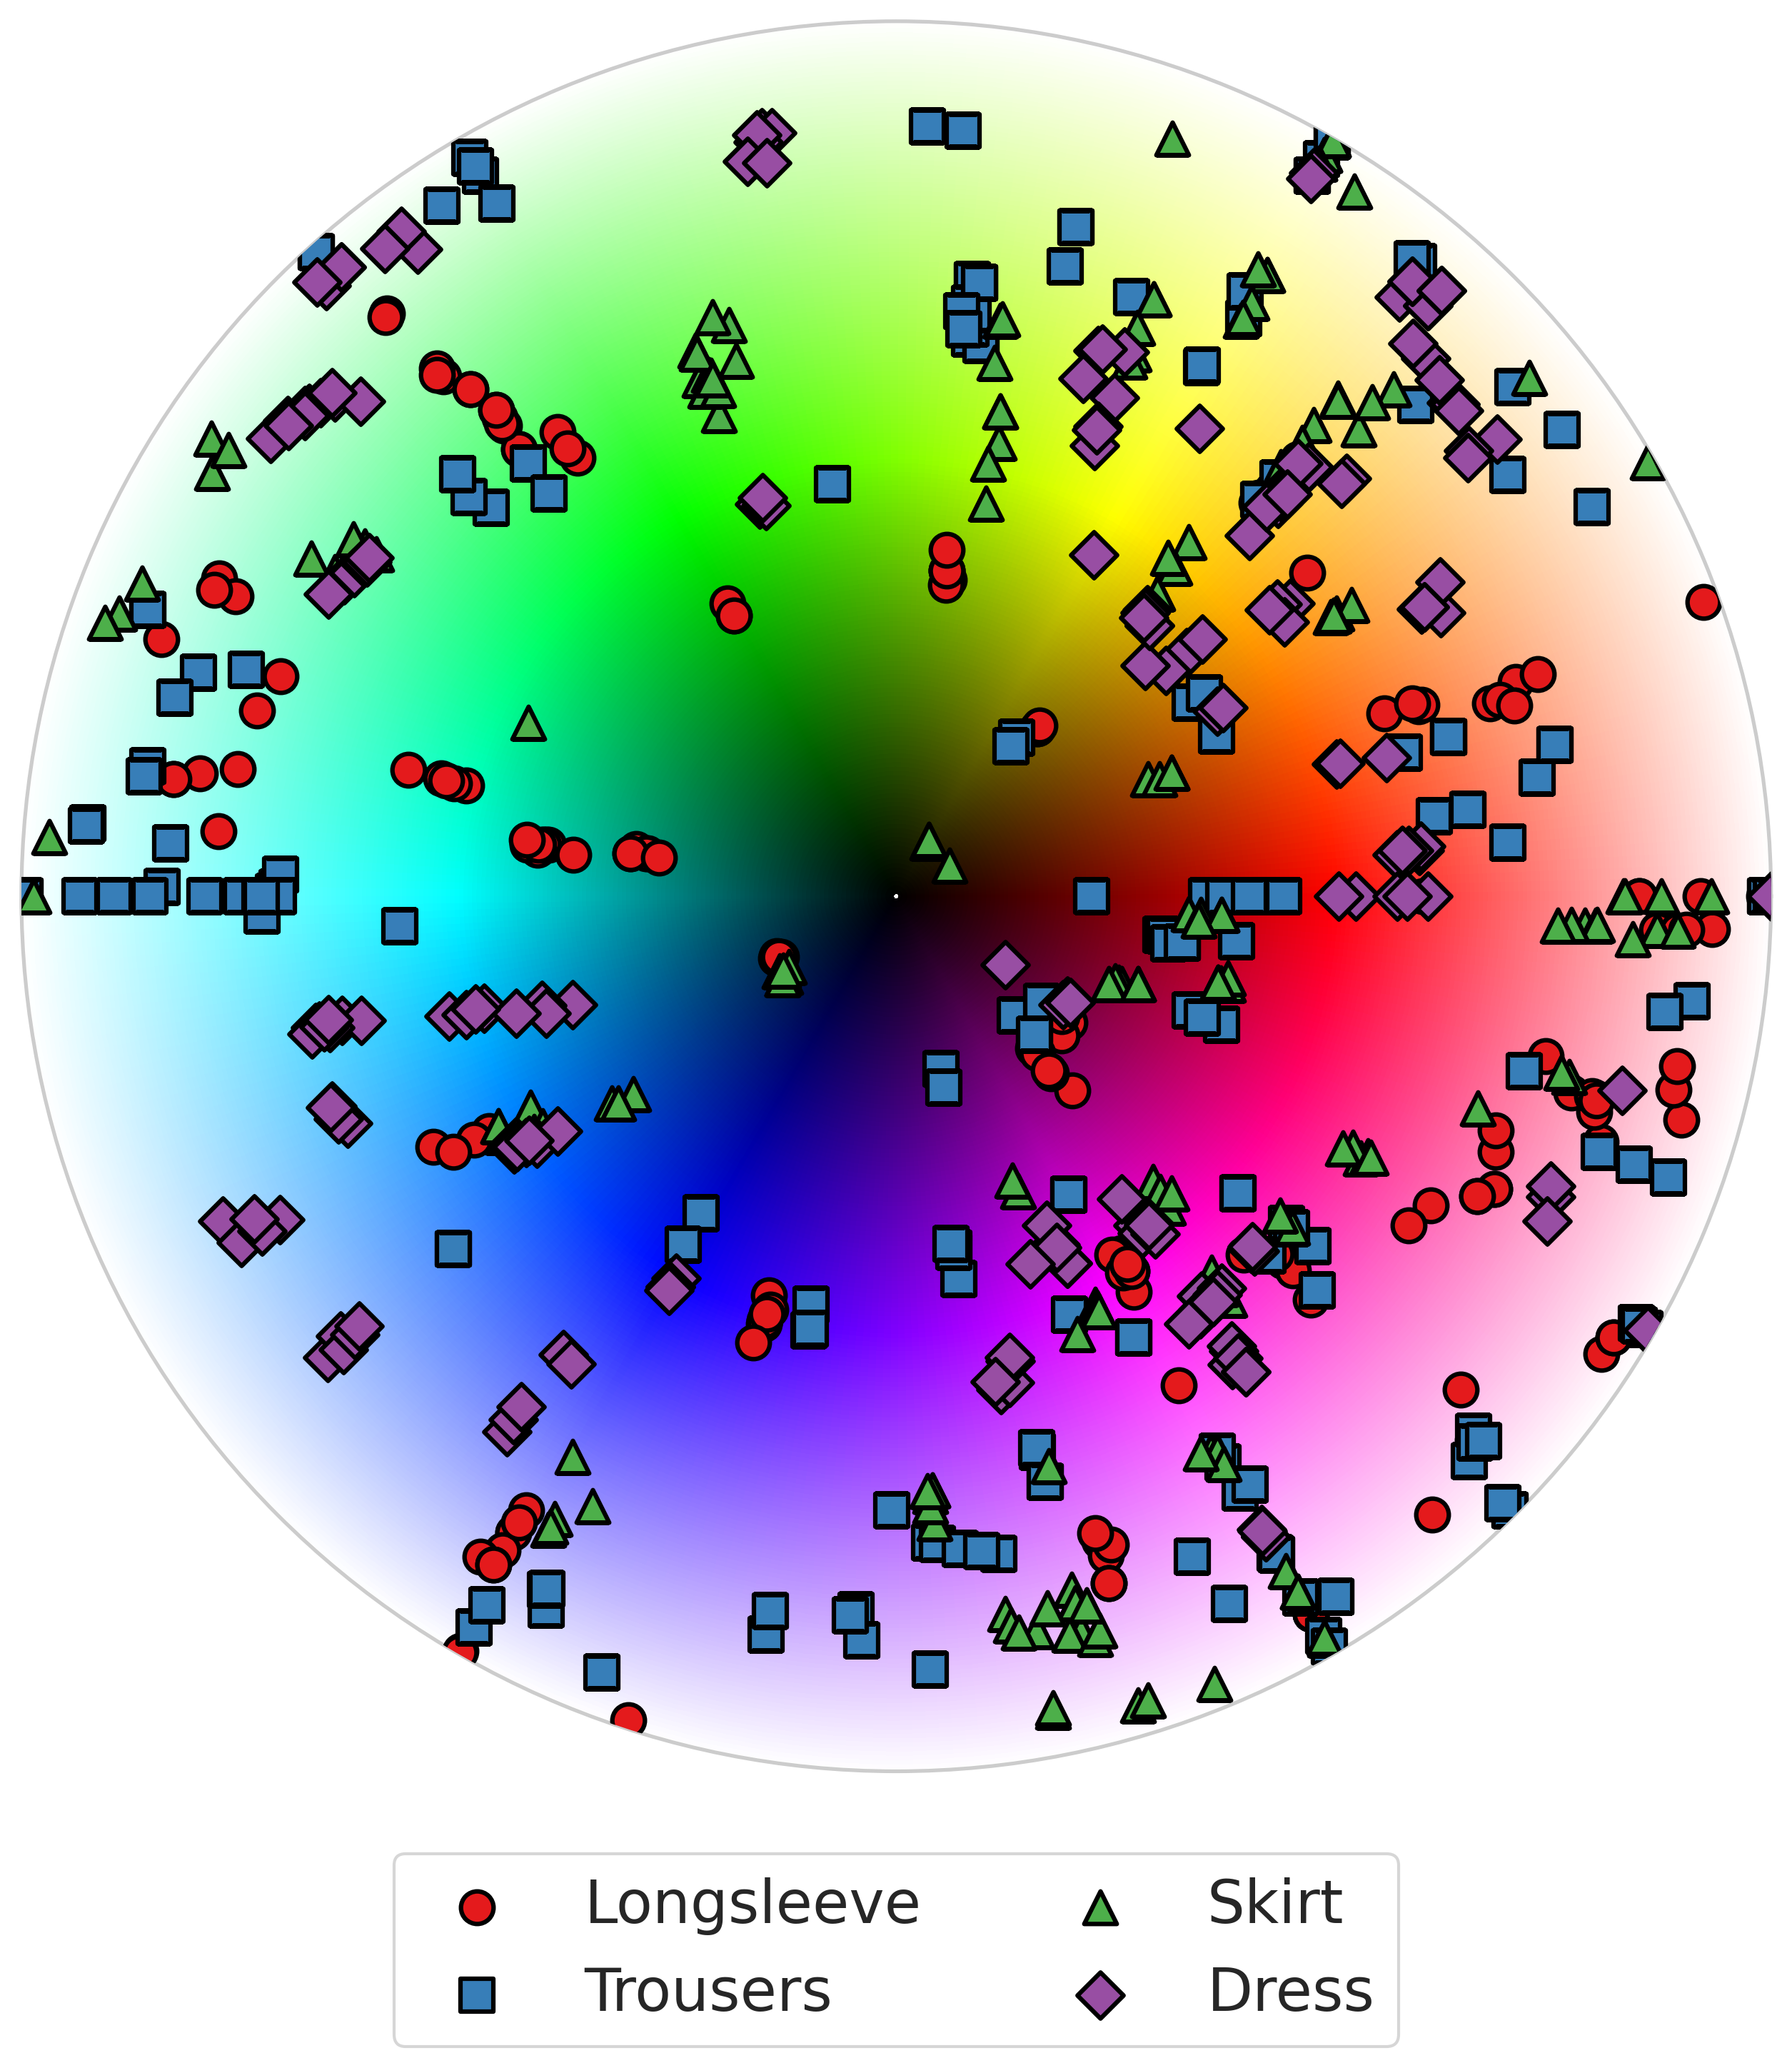
\includegraphics[width=\linewidth]{plots/colour_distribution.png}
        \caption{Colour Distribution}
        \label{fig:colour-distribution}
    \end{subfigure}
    \caption{\addinfo{The initial state distribution of simulation garments.}}
    \label{fig:garment-distribution}
\end{figure*}


\addinfo{All models are trained for 50,000 update steps, validating every 1,000 steps to save the best-performing checkpoint. Simulation training trials are 200, validation trials are 10, and evaluation trials are 30; each trajectory in the dataset is up to 20-step long. We compare the performance of different checkpoints through a custom heuristic that balances terminal flattening quality with policy efficiency. Specifically, we compute a combined performance score for each checkpoint by summing its average final NC and average Max IoU across the validation trials. If competing checkpoints both achieve a highly proficient combined score exceeding 1.90 (out of a theoretical maximum of 2.0), we prioritise the policy that completes the task in fewer average steps to encourage efficiency. Otherwise, we strictly select the checkpoint with the highest combined score.}

\subsection{Comparison of \text{LaGarNet} against Other Neural Controllers} \label{sec:comp-sota}

\begin{table*}[t!]
\caption{Numerical comparison of different learning-based pick-and-place (\text{PnP}) controllers on longsleeved T-shirts in simulation. We only enable the \addinfo{single-arm} PnP primitive of the off-the-shelf \text{ClothFunnels} \cite{canberk2023cloth} \addinfo{to ensure that all model operate in a consistent environment.} We train both \text{PlaNet-ClothPick} and \text{LaGarNet} with the RGB-to-Mask setup on the same task-focused and all-garments datasets, yet with their own reward functions and network architectures. We train the behaviour cloning methods \text{Diffusion Policy} \cite{kadi2025draper, chi2023diffusionpolicy} with \addtypo{200} human demonstrations. Mesh-based planning method, $\dagger$ VCD \cite{lin2020softgym} , reports to reach 83.8 $\pm$ 45 \% NI and 96 $\pm$ 21.8 \% NC for T-shirt flattening in simulation within 20 steps; \addadvantage{however, its improved successor, MEDOR \cite{huang2022mesh}, stably outperforms it in all scenarios.} \addadvantage{We test the off-the-shelf MEDOR in our evaluation trials but with their simulation setup. We highlight the top \addadvantage{three} values for each \addadvantage{metric} and action  \addadvantage{step} with green, yellow\addadvantage{,} and red \addadvantage{backgrounds, respectively}.} The proposed All-Garments \text{LaGarNet} outperforms all compared algorithms \addadvantage{;} it reaches a similar performance \addadvantage{to the} SoTA mesh-based method MEDOR\addadvantage{,} and even slightly outperforms human \addadvantage{experts} from 10-20 steps.}
\label{tab:longsleeve-flattening}
\centering
\resizebox{\textwidth}{!}{%
\begin{tabular}{p{1.8cm}|p{1.6cm}p{1.7cm}p{1.9cm}p{1.9cm}|p{2.1cm}p{1.9cm}p{2.2cm}||c}
Longsleeved T-shirt & Task-Specific SAC & Task-Specific ClothFunnels & Task-Specific  Diffusion Policy & Task-Specific LaGarNet & All-Garment PlaNet-ClothPick & All-Garment MEDOR & Ours: All-Garment LaGarNet & Human \\
\hline
NI $\uparrow$ (5 steps) & 41.4 $\pm$ 26.0 & 34.4 $\pm$ 19.5 & 39.7 $\pm$ 21.4 & 37.4 $\pm$ 22.1 & 42.6 $\pm$ 20.6 & \cellcolor{red!25}61.0 $\pm$ 17.7 & \cellcolor{yellow!25}61.6 $\pm$ 21.9 & \cellcolor{green!25}63.0 $\pm$ 20.0 \\
NC $\uparrow$ & 73.2 $\pm$ 11.5 & 68.8 $\pm$ 11.7 & 71.8 $\pm$ 11.0 & 71.0 $\pm$ 11.3 & 72.9 $\pm$ 10.7 & \cellcolor{yellow!25}81.7 $\pm$ 8.3 & \cellcolor{red!25}81.0 $\pm$ 12.4 & \cellcolor{green!25}81.8 $\pm$ 10.7 \\
Max IoU $\uparrow$ & 62.2 $\pm$ 7.9 & 58.3 $\pm$ 8.6 & 61.8 $\pm$ 8.0 & 60.3 $\pm$ 7.5 & 60.5 $\pm$ 8.0 & \cellcolor{green!25}71.1 $\pm$ 6.5 & \cellcolor{red!25}67.3 $\pm$ 8.8 & \cellcolor{yellow!25}68.1 $\pm$ 8.3 \\
SR $\uparrow$ & \cellcolor{red!25}1/30 & 0/30 & 0/30 & 0/30 & \cellcolor{red!25}1/30 & \cellcolor{yellow!25}2/30 & \cellcolor{yellow!25}2/30 & \cellcolor{green!25}3/30 \\
\hline
NI $\uparrow$ (10 steps) & 53.4 $\pm$ 26.7 & 44.8 $\pm$ 19.2 & 56.9 $\pm$ 25.0 & 71.8 $\pm$ 24.1 & 71.2 $\pm$ 21.7 & \cellcolor{yellow!25}83.0 $\pm$ 17.1 & \cellcolor{green!25}86.5 $\pm$ 14.5 & \cellcolor{red!25}82.4 $\pm$ 14.9 \\
NC $\uparrow$ & 79.2 $\pm$ 10.2 & 73.7 $\pm$ 11.3 & 80.1 $\pm$ 11.6 & 87.1 $\pm$ 11.3 & 86.5 $\pm$ 10.3 & \cellcolor{yellow!25}92.2 $\pm$ 7.7 & \cellcolor{green!25}93.2 $\pm$ 8.1 & \cellcolor{red!25}91.2 $\pm$ 8.3 \\
Max IoU $\uparrow$ & 66.5 $\pm$ 7.2 & 62.9 $\pm$ 8.2 & 69.1 $\pm$ 9.8 & 72.5 $\pm$ 8.8 & 70.0 $\pm$ 7.4 & \cellcolor{red!25}76.9 $\pm$ 6.2 & \cellcolor{yellow!25}77.5 $\pm$ 5.4 & \cellcolor{green!25}78.3 $\pm$ 6.8 \\
SR $\uparrow$ & 1/30 & 0/30 & 5/30 & \cellcolor{red!25}7/30 & 4/30 & 6/30 & \cellcolor{green!25}12/30 & \cellcolor{yellow!25}10/30 \\
\hline
NI $\uparrow$ (20 steps) & 63.9 $\pm$ 24.6 & 57.3 $\pm$ 21.9 & 83.4 $\pm$ 17.9 & 85.7 $\pm$ 17.6 & 86.2 $\pm$ 16.5 & \cellcolor{green!25}96.6 $\pm$ 10.4 & \cellcolor{yellow!25}94.4 $\pm$ 11.5 & \cellcolor{red!25}94.3 $\pm$ 8.8 \\
NC $\uparrow$ & 83.9 $\pm$ 9.6 & 79.8 $\pm$ 11.5 & 92.4 $\pm$ 8.4 & 93.4 $\pm$ 8.2 & 93.7 $\pm$ 7.5 & \cellcolor{green!25}98.3 $\pm$ 5.3 & \cellcolor{red!25}97.0 $\pm$ 6.5 & \cellcolor{yellow!25}97.2 $\pm$ 4.8 \\
Max IoU $\uparrow$ & 69.6 $\pm$ 6.1 & 66.5 $\pm$ 8.8 & 78.3 $\pm$ 7.9 & 77.8 $\pm$ 8.1 & 74.1 $\pm$ 6.5 & \cellcolor{yellow!25}82.2 $\pm$ 6.0 & \cellcolor{red!25}81.2 $\pm$ 4.5 & \cellcolor{green!25}85.5 $\pm$ 5.3 \\
SR $\uparrow$ & 2/30 & 2/30 & 13/30 & 16/30 & 7/30 & \cellcolor{red!25}21/30 & \cellcolor{yellow!25}23/30 & \cellcolor{green!25}26/30 \\
\hline
NI $\uparrow$ (30 steps) & 70.9 $\pm$ 18.6 & 64.0 $\pm$ 20.7 & 91.3 $\pm$ 15.4 & 94.6 $\pm$ 10.7 & 94.3 $\pm$ 9.4 & \cellcolor{green!25}98.3 $\pm$ 8.6 & \cellcolor{red!25}96.7 $\pm$ 8.6 & \cellcolor{yellow!25}97.8 $\pm$ 6.4 \\
NC $\uparrow$ & 86.9 $\pm$ 7.5 & 82.8 $\pm$ 10.4 & 96.3 $\pm$ 5.9 & 97.4 $\pm$ 5.3 & 97.4 $\pm$ 4.6 & \cellcolor{green!25}99.1 $\pm$ 4.3 & \cellcolor{red!25}98.2 $\pm$ 4.8 & \cellcolor{yellow!25}98.8 $\pm$ 3.6 \\
Max IoU $\uparrow$ & 71.4 $\pm$ 5.5 & 68.5 $\pm$ 8.7 & \cellcolor{red!25}83.7 $\pm$ 5.6 & 82.3 $\pm$ 6.0 & 78.3 $\pm$ 5.0 & \cellcolor{yellow!25}84.1 $\pm$ 4.6 & 82.7 $\pm$ 3.8 & \cellcolor{green!25}87.7 $\pm$ 4.3 \\
SR $\uparrow$ & 2/30 & 2/30 & \cellcolor{red!25}24/30 & \cellcolor{red!25}24/30 & 11/30 & \cellcolor{yellow!25}26/30 & \cellcolor{yellow!25}26/30 & \cellcolor{green!25}29/30 \\
\bottomrule
\end{tabular}}

\end{table*}



\addIncrementalg{This section compares various state-of-the-art (SoTA) methods for single-arm pick-and-place (PnP) in simulation. We first introduce our simulation setup (Section \ref{sec:simulation}), followed by our rationale for selecting and evaluating various SoTA baselines (Section \ref{sec:baseline}). Then, we analyse the primary and secondary performance of these methods (Section \ref{sec:sota-result}).}

\subsubsection{Simulation Setup} \label{sec:simulation}

We develop \text{LaGarNet} using the garment simulation environment from Canberk et al.~\cite{canberk2023cloth} which is built on SoftGym \cite{lin2020softgym} and PyFlex physics engine \cite{li2018learning}. Following the real-world adaptation strategy of the \text{DRAPER} methodology \cite{kadi2025draper}, \addadvantage{we extend the simulation to include} misgrasping and multi-layer grasping scenarios\addadvantage{,} inherent to \addadvantage{simple} parallel grippers. We focus on simulated longsleeved T-shirts, trousers, dresses\addadvantage{,} and skirt objects selected by Canberk et al. from \addadvantage{the} commonly employed \text{Cloth3D} dataset \cite{bertiche2020cloth3d} (see Figure \ref{fig:sim-train-init}). Please see the Table \ref{tab:sim-config} for our simulation configuration. Following Canberk et al., we scale the garments by a factor of 0.8 and set the a simulated top-down camera height with a completely dark background for vision rendering. They split the generated initial garments into ``hard'' and ``easy'' categories\addadvantage{,} where the former is more crumpled and the latter is more flattened; we use 30 ``hard'' initial states placed within the defined workspace of the gripper for evaluation. Please see Figure \ref{fig:garment-distribution} for the distribution of our simulation garments.


\subsubsection{Baseline Methods} \label{sec:baseline} 

We benchmark our model-based reinforcement learning (RL) method \textbf{LaGarNet} against \addadvantage{past RSSM approaches like \textbf{PlaNet-ClothPick}} \cite{kadi2024planet} and the off-the-shelf task-specific model-free method \textbf{ClothFunnels} \cite{canberk2023cloth} \addadvantage{using} its single-arm PnP primitives. We also compare against the state-of-the-art mesh-based planning method \textbf{MEDOR} \cite{huang2022mesh} \addadvantage{ with its own simulation setup (see Table \ref{tab:sim-config})---we make sure our flattened garments is fully observable, looking similar to their own trial distribution.} We also compare LaGarNet against the advanced deep behaviour cloning method \text{Diffusion Policy}\addadvantage{,} \addadvantage{adapted} for \addadvantage{the} PnP cloth-shaping domain \cite{chi2023diffusionpolicy, kadi2025draper}.  

All trained methods apart from \text{ClothFunnels} and \text{MEDOR} employ the vision processing strategy \addadvantage{from the} \text{DRAPER} framework to achieve simulation-to-reality transfer \cite{kadi2024mjtn}; this strategy attempts to align  real and synthetic RGB observations, \addadvantage{applying} real-world adapt\addadvantage{at}ion and domain randomisation in simulation\addadvantage{,} as well as a refined grasping procedure to reduce failures. Whil\addadvantage{e} we train \text{Diffusion Policy} on \addtypo{200} human expert trajectories, we let \text{LaGarNet} and \text{PlaNet-ClothPick} learn from \addtypo{5} thousand episodes (i.e., \addtypo{100} thousand transitional steps) generated from \addadvantage{our} data-collection strategy. \addadvantage{\text{PlaNet-ClothPick} uses similar set of hyperparameters as \text{LaGarNet} but with different reward function and without goal observations.} \addadvantage{The all-garment}  variants of these methods adopts the trajectories from all four garment types\addadvantage{, whilst keeping the same data size as task-specific datasets} \addadvantage{We conduct human experiments} through a PnP window interface operating directly on observation images both in simulation and the real world.

\begin{figure*}[t!]
    \centering
    
\includegraphics[width=1.0\linewidth]{plots/multi_arena_radar.png}
    \caption{\addadvantage{Simulation performance of different policies on all four garment types by action step 20. Our method \text{LaGarNet} consistently outperform\addadvantage{s} \addadvantage{the} baseline all-garment \text{PlaNet-ClothPick} and task-specific \text{Diffusion Policy} on each garment type.}}
    \label{fig:sim-lagarnet-results}
\end{figure*}

\begin{table*}[t!]
    \centering
    \caption{\addadvantage{Secondary comparison of computational requirements and data efficiency across garment flattening baselines. $\dagger$ represents the reported values in the \addadvantage{original} paper. \text{ClothFunnels} uses a machine with 4 NVIDIA RTX3090s. Our hardware setup for all timing and parameter evaluations \addadvantage{is}: Ubuntu 24.04.4 LTS, NVIDIA GeForce RTX 3090 Ti GPU, AMD Ryzen 9 5900X 12-Core Processor (2 threads per core), and 64GB RAM. Whist mesh-based method requires substantially shorter data collection time, our LaGarNet method demands much less network parameters and faster training and per-step inference time.}}
    \label{tab:efficiency-comparison}
    \resizebox{1.0\textwidth}{!}{%
    \begin{tabular}{lccccc}
    \toprule
    \textbf{Method} & \textbf{Data Size} & \textbf{Network Parameters (M)} & \textbf{$\sim$ Inference Time (s)} & \textbf{Data Collection Time (hrs)} & \textbf{Training Time (hrs)} \\
    \midrule
    ClothFunnels & 12,500 eps $\times$ 10 $P\&P$ $\dagger$ & 12.6 & 2 &  48 $\dagger$ &  48 $\dagger$ \\
    MEDOR & 5000 P\&P $\times$ 100 low-level steps $\dagger$ & 37.5 &  103 & 0.64 & 144 $\dagger$ \\
    % Task-Specific JA-TN & 200 eps $\times$ 20 $P\&P$  & 29.5 &  0.13 &  22 &  17 \\
    Task-Specific Diffusion Policy & 200 eps $\times$ 20 $P\&P$ & 83.7 &  1.5 &  22 & 35 \\
    All-Garment PlaNet-ClothPick & 5,000 eps $\times$ 20 $P\&P$ & 6.3 &  4 &  4 $\times$ 22 + max(75, 34) = 163 &  31 \\
    All-Garment LaGarNet & 5,000 eps $\times$ 20 $P\&P$ & 7.11 &  6 &  4 $\times$ 22 + max(75, 34) = 163 &  33 \\
    \bottomrule
    \end{tabular}
    }
\end{table*}

\subsubsection{Results} \label{sec:sota-result}

\addadvantage{Table \ref{tab:longsleeve-flattening} summarises the flattening performance across all evaluated baselines. Overall, our proposed All-Garment LaGarNet achieves results comparable to the state-of-the-art mesh-based planning method, MEDOR, and closely matches human performance. However, human experts maintain the highest success rates at step 30; this is primarily driven by their superior ability to achieve a higher Max IoU compared to current learning-based methods. Furthermore, when trained on an equivalent volume of data, the All-Garment LaGarNet consistently outperforms the Task-Specific LaGarNet (which is trained exclusively on longsleeve data). This demonstrates that our architecture actively benefits from morphological diversity, successfully leveraging multi-garment data to improve task-specific performance. Interestingly, given a sufficiently long execution horizon (e.g., 30 steps), the task-specific Diffusion Policy---despite being trained on only 200 human demonstrations and struggling at shorter horizons---eventually recovers to achieve highly competitive results. Figure \ref{fig:sim-lagarnet-results} demonstrates that the single-policy \text{LaGarNet} successfully generalises, achieving above 95\% NC across all evaluated garment types at action step 20, though higher success rates on skirts and dresses indicate a bias toward simpler topologies.}
\addadvantage{Furthermore, Table \ref{tab:efficiency-comparison} contextualises these results through secondary metrics, revealing a crucial trade-off. While MEDOR achieves high Max IoU, it requires a computationally prohibitive inference time of $\sim$103 seconds per step and relies on 37.5M network parameters. In contrast, All-Garment \text{LaGarNet} demonstrates superior computational efficiency, requiring only 7.11M parameters and executing in roughly 6 seconds per step—making it substantially more suitable for real-world deployment. The behaviour cloning baseline, \text{Diffusion Policy}, while fast, requires significantly more parameters (83.7M) and ultimately falls short of \text{LaGarNet}'s flattening success rate (SR).}
\begin{figure*}[t!]
    \centering
    
    % Subfigure A: Progression Plot
    \subfloat[\centering Validation Trials \label{fig:diffusion-human-val}]{
        
\includegraphics[width=0.28\textwidth]{plots/progression_nc_vs_iou.png}
    }\hfill
    % Subfigure B: Radar Chart
    \subfloat[\centering Evaluation Trials \label{fig:diffusion-human-eval}]{
        
\includegraphics[width=0.21\textwidth]{plots/metrics_radar.png}
    }\hfill
    % Subfigure C: The Table
    \subfloat[\centering Architectural Ablations \label{tab:comp-diff-lagarnet}]{
        \resizebox{0.45\textwidth}{!}{
            \begin{tabular}{lcccc}
            \toprule
            Method & SR & Max IoU & NC & NI \\
            \midrule
            GC-DP & 40.0 & 77.6 $\pm$ 6.6 & 89.7 $\pm$ 2.5 & 77.8 $\pm$ 4.8 \\
            GC-DP-Comp & 25.0 & 76.0 $\pm$ 6.6 & 87.2 $\pm$ 1.1 & 72.7 $\pm$ 2.7 \\
            LaGarNet-Comp & 5.0 & 69.1 $\pm$ 2.4 & 77.3 $\pm$ 5.0 & 49.4 $\pm$ 10.9 \\
            LaGarNet-RSSM & 52.5 & 82.0 $\pm$ 3.3 & 92.9 $\pm$ 0.9 & 84.6 $\pm$ 3.0 \\
            
            GC-RSSM-DP & 6.7 & 68.6 $\pm$ 3.4 & 77.4 $\pm$ 2.3 & 50.1 $\pm$ 5.0 \\
            LaGarNet-CNN-DP & 8.3 & 70.0 $\pm$ 3.6 & 78.2 $\pm$ 3.4 & 51.8 $\pm$ 6.5 \\

            \rowcolor{green!20} LaGarNet & 75.0 & 84.5 $\pm$ 3.0 & 95.4 $\pm$ 1.4 & 90.1 $\pm$ 3.4 \\
            \bottomrule
            \end{tabular}
        }
    }
    
    \caption{\addadvantage{Performance comparison between Diffusion Policy and LaGarNet on the simulated longsleeve environment. \textbf{(a)} Validation performance over the course of 50,000 training steps for task-specific Diffusion Policies trained with varying human demonstrations. To highlight the underlying training trends amidst step-to-step variance, the bold lines represent an Exponential Moving Average (EMA, span = 15) of the success rate, while the raw, unsmoothed data is plotted faintly in the background. \textbf{(b)} A radar chart illustrating the evaluation performance of these policies across the four primary metrics. The All-Garment LaGarNet demonstrates highly stable, sample-efficient training and achieves superior evaluation performance compared to the behaviour cloning diffusion policy baselines. \textbf{(c)} Performance comparison of various architectural ablations by action step 20. All values are aggregated across 120 evaluation episodes (30 trials for each of the four garment types). The standard LaGarNet, trained on 5,000 episodes of mixed-quality transitional trajectories, shows substantially better performance compared to all variants of the Diffusion Policy, which are trained on an equivalent volume of success-only trajectories.}} 
    \label{fig:diff-vs-lagarnet-performance-combined}
\end{figure*}





\subsection{Diffusion Policy vs. LaGarNet}  \label{sec:comp-diff}


\addadvantage{Building upon the simulation setup introduced in Section \ref{sec:simulation}, we further investigate LaGarNet's performance advantage over Diffusion Policy baselines. Specifically, we aim to determine whether LaGarNet's superiority stems from its explicit forward planning, its ability to learn from extended temporal context windows, or simply from data scalability. First, we examine how scaling human demonstrations impacts the performance of a task-specific Diffusion Policy, as illustrated in Figure \ref{fig:diffusion-human-val} and \ref{fig:diffusion-human-eval}. Next, we design various ablated baselines (Section \ref{sec:diff-baselines}) to conduct a granular comparison between LaGarNet and Diffusion Policies. Finally, we analyse the primary performance metrics of these baselines (Section \ref{sec:diff-result}).} 


\subsubsection{Baselines} \label{sec:diff-baselines}

\addadvantage{To isolate the specific architectural components that contribute to LaGarNet's superiority over Diffusion Policies, we design the following baseline policies:}

\addadvantage{a) \textbf{GC-DP}: A Goal-Conditioned Diffusion Policy (Section \ref{sec:diffusion}) that concatenates the current and goal RGB images as input. This model is trained on 5,000 episodes of diffusion-induced, success-only data spanning all garment types.}

\addadvantage{b) \textbf{GC-DP-Comp}: A variant of GC-DP trained with hyperparameters modified to align with LaGarNet for a fair comparison. Notably, it replaces the original ResNet-18 encoder with PlaNet's CNN encoder. Similar to LaGarNet, it concatenates the embeddings of the current and goal observations before passing them to the downstream networks, and the observation sequence length is increased from 1 to 4.}

\addadvantage{c) \textbf{LaGarNet-Comp}: A variant of LaGarNet trained with a constrained set of hyperparameters for direct comparison against the diffusion baselines. The most significant change is the reduction of its training sequence length from 50 to 4.}

\addadvantage{d) \textbf{LaGarNet-RSSM}: The standard LaGarNet architecture utilizing its full RSSM dynamics model.}

\addadvantage{e) \textbf{GC-RSSM-DP}: A variant of GC-DP-Comp that utilizes LaGarNet's pre-trained latent dynamics model. The conditioning dimension of the noise predictor network is set to 360. At each step, the historical memory is wiped by initialising the previous latent state to zero. The current observation's posterior latent state is then obtained by feeding a ``no-op'' action into the latent dynamics model. Both the vision encoder and the dynamics model of the pre-trained GC-RSSM are frozen during training.}

\addadvantage{f) \textbf{LaGarNet-CNN-DP}: A variant of GC-DP-Comp that utilizes LaGarNet's pre-trained vision encoder. The observation embedding dimension becomes 2048, formed by concatenating the current and goal observation embeddings from LaGarNet. The vision encoder is frozen during training.}

\addadvantage{We train all policies using the appropriate hyperparameters detailed in Table \ref{tab:all-hyperparameters}.c, applying consistent data augmentation schemes across all methods (Section \ref{sec:data-aug}).}

\subsubsection{Results} \label{sec:diff-result}

\addadvantage{As detailed in Table \ref{tab:comp-diff-lagarnet}, LaGarNet demonstrates a substantial performance advantage over the baseline diffusion approaches, achieving a success rate (SR) of 72.5\% compared to the 40.0\% yielded by GC-DP. This disparity is particularly notable given that LaGarNet is trained on 5,000 episodes of mixed-quality, transitional data, whereas GC-DP utilises an equivalent volume of strictly success-only trajectories. The superior performance of LaGarNet across all metrics—including a peak Normalised Coverage (NC) of 96.1 $\pm$ 1.1\% and Normalised Improvement (NI) of 91.3 $\pm$ 2.3\%—strongly suggests that its model-based architecture is fundamentally better suited for the garment flattening domain. }
\addadvantage{In addition, the stark performance degradation among the ablated variants underscores the critical importance of LaGarNet's extended temporal context. When LaGarNet is artificially constrained to a shorter sequence length of 4 (LaGarNet-Comp), its success rate collapses to a mere 5.0\%. This indicates that leveraging a world model trained over a long context horizon is essential for capturing the complex, long-horizon dynamics of deformable object manipulation. Also, when switching back to the oringal RSSM (LaGarNet-RSSM) as the form of latent dynamic learning, the success rate readuces around 30\% percent, marking the importance of the goal in our algorithm. }

\addadvantage{Furthermore, attempts to transplant LaGarNet's pre-trained visual or latent representations into the diffusion framework (LaGarNet-CNN-DP and GC-RSSM-DP) resulted in exceptionally poor success rates of 8.3\% and 6.7\%, respectively. This ablation reveals a fundamental limitation of the baseline diffusion approaches in this context: their efficacy relies almost entirely on an end-to-end, reactive mapping from observations to action noise, rather than on a structured understanding of environment dynamics. Because the diffusion policy lacks the architectural capacity to explicitly reason over future states, it fails to meaningfully exploit these rich, pre-trained latent representations. In contrast, LaGarNet successfully leverages its decoupled world model to anticipate and plan for the complex, non-rigid deformations of garments. These results strongly indicate that LaGarNet's model-based paradigm—grounded in explicit forward planning—is vastly superior to the purely reactive, data-hungry nature of standard diffusion models for long-horizon garment manipulation tasks.}
\subsection{Ablation Study on \text{LaGarNet}} \label{sec:abl}

\begin{figure*}[t!]
    \centering
    
    % --- LEFT COLUMN: Ablation Plots and Table ---
    \begin{minipage}[t]{0.52\textwidth}
        \vspace{0pt} % <-- TRICK: Forces top alignment of the minipage content
        \centering
        % Top Row (Left Column): Ablation Plots side-by-side
        \subfloat[\centering Latent Dynamic and Goal Ablation \label{fig:goal-ablation}]{
            
\includegraphics[width=0.46\linewidth]{plots/ablation_latent_bar.png}
        }
        \subfloat[\centering Reward Ablation \label{fig:reward-ablation}]{
            
\includegraphics[width=0.46\linewidth]{plots/ablation_reward_bar.png}
        }        
        
        \vspace{0.4cm} % Vertical spacing between plots and the table

        \subfloat[\centering Data Size Ablation. \label{fig:datasize-ablation}]{
            
\includegraphics[width=0.46\linewidth]{plots/ablation_data_size_line.png}
        } 
        \subfloat[\centering Data Composition Ablation \label{fig:dataratio-ablation}]{
            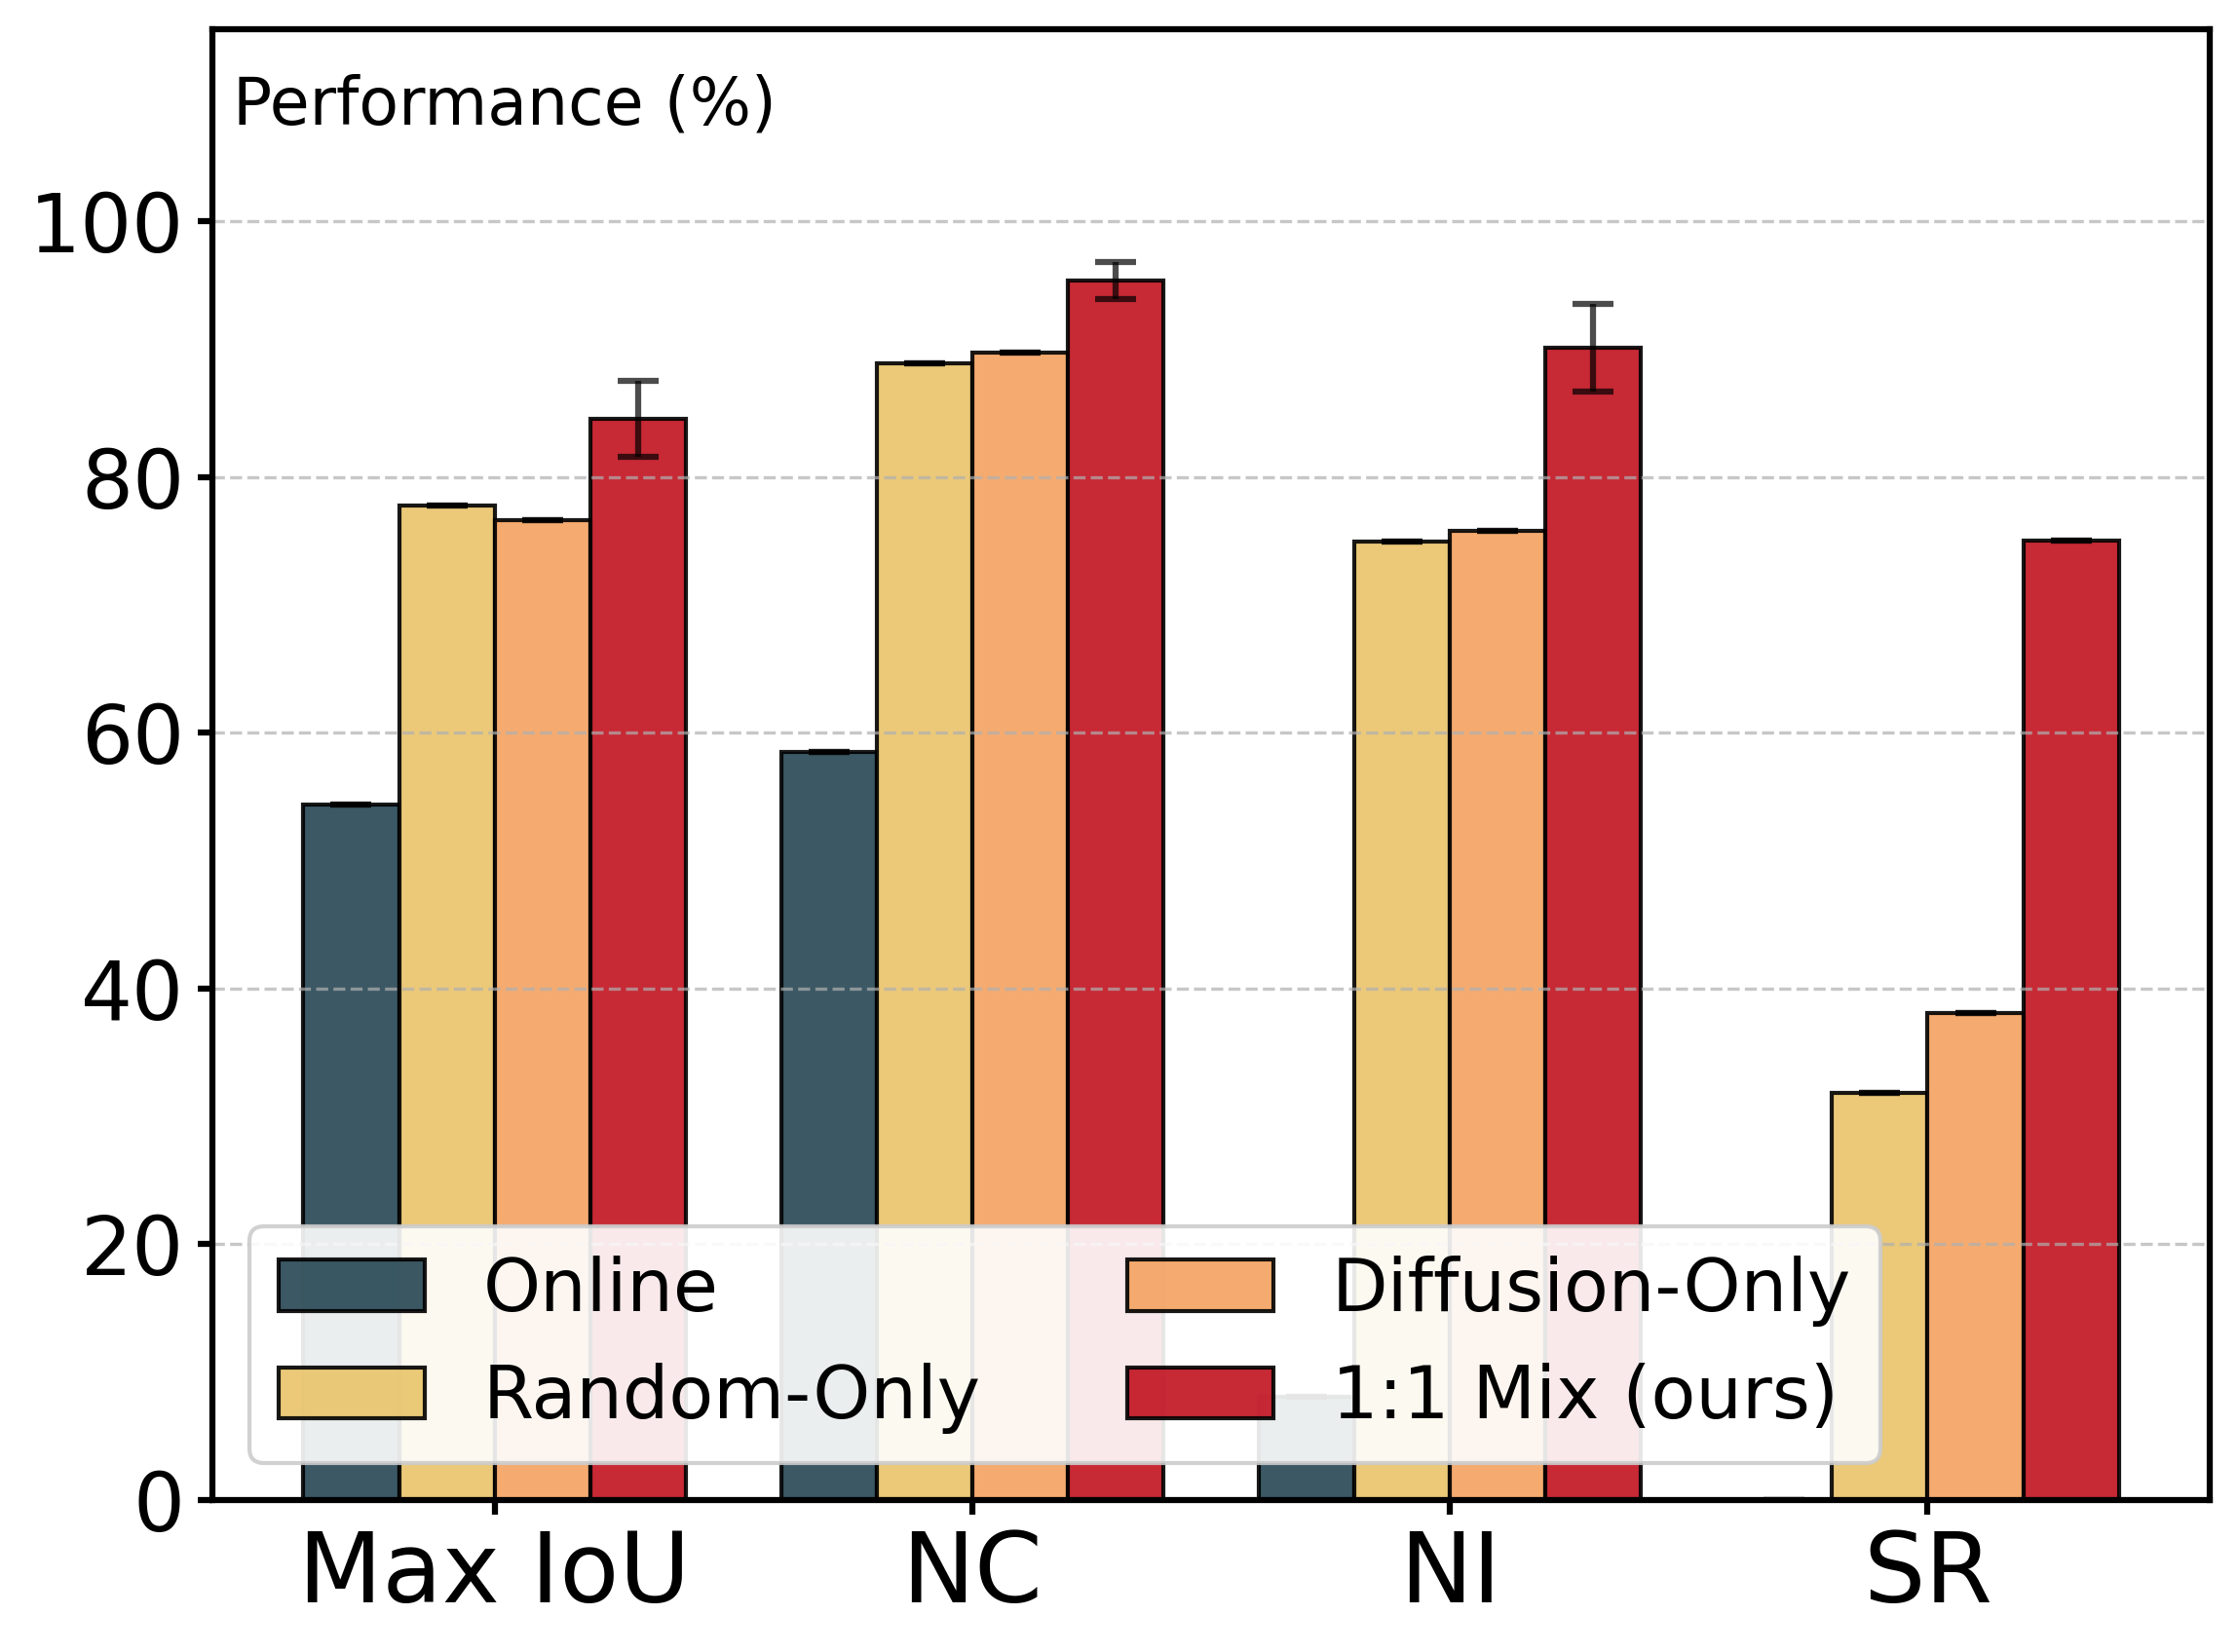
\includegraphics[width=0.46\linewidth]{plots/ablation_data_ratio_bar.png}
        } 
       
    \end{minipage}\hfill % <-- Spreading out the columns
    % --- RIGHT COLUMN: Reconstruction Image ---
    \begin{minipage}[t]{0.48\textwidth}
        \vspace{0pt} % <-- TRICK: Forces top alignment of the minipage content
        \centering
        \subfloat[\centering Observation reconstruction quality \label{fig:recon-quality}]{
            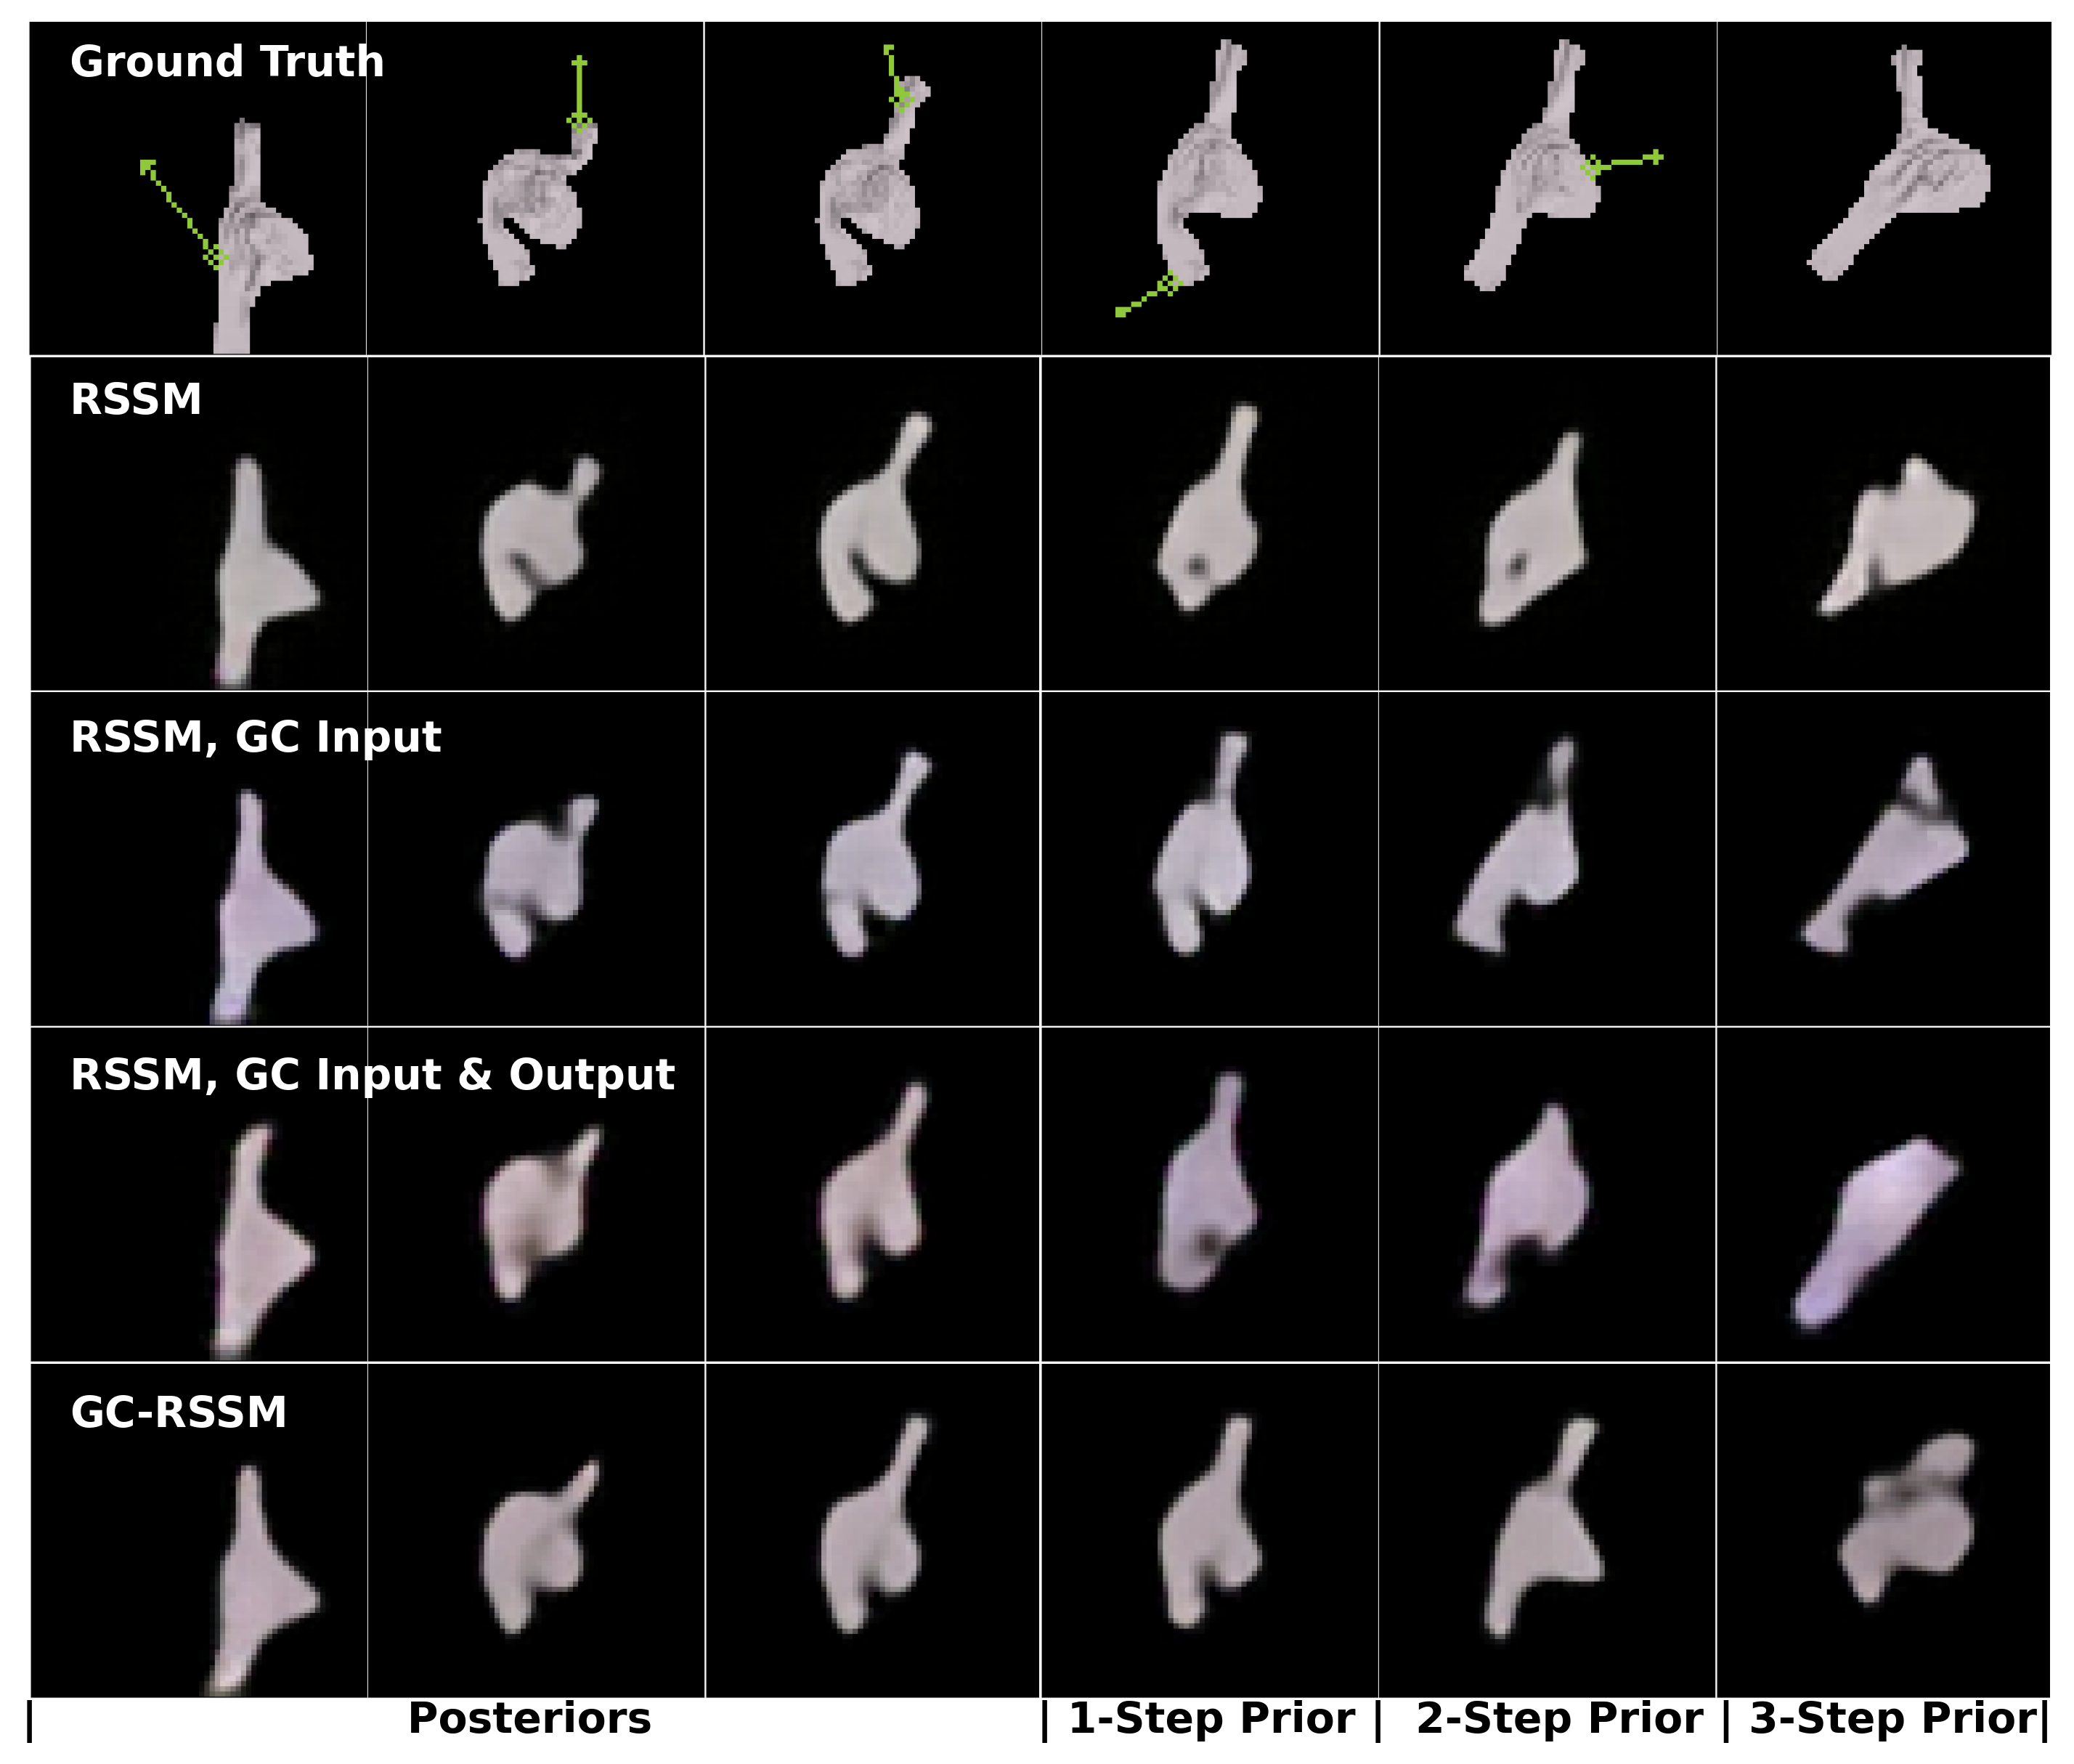
\includegraphics[width=\linewidth]{plots/recon-all-garments.png}
        }
    \end{minipage}
    
    \caption{\addadvantage{Comprehensive ablation study for LaGarNet in simulation environments. \textbf{(a, b, c, and d)} Ablation study using the all-garment LaGarNet models; all components of LaGarNet are essential for the success of this policy in garment flattening. \textbf{(e)} Observation reconstruction quality of models from Figure (a); each grid is a 64$\times$64 RGB image. The green arrows in the first row represent pick-and-place actions; our GC-RSSM model demonstrates a superior ability to track garment sleeves in prior steps compared to other RSSM variants.}}
    \label{fig:ablation-and-recon-combined}
\end{figure*}

\begin{table}[t!]
\caption{Quantitative results for RGB image reconstruction quality from various world models are presented. We evaluate the visual quality and similarity of generated images using Mean Squared Error (MSE) and Structural Similarity Index (SSIM) \cite{wang2004image}. SSIM is especially useful as it evaluates local structure and contrast, which are directly affected by blurring. All values are multiplied by 100 for clearer comparison. Each value represents the aggregate average over 10 trials for each of the 4 garments. All these models are based on same internal hyperparameters; the differences lie in how the models are structured and how their inputs and outputs differ. Our goal-conditioned recurrent state-space model (GC-RSSM) shows a improvement of reducing blurriness on the multi-step prior reconstructed images.}
\label{tab:recon-quality}
\resizebox{0.47\textwidth}{!}{
\setlength{\tabcolsep}{2pt} % Default is 6pt, try 2pt or adjust as needed
\renewcommand{\arraystretch}{1.1} % Optional: slightly increase row height for readability
\begin{tabular}{l|cc|cc|cc|cc}
 & \multicolumn{2}{c|}{Posterior} & \multicolumn{2}{c|}{Prior 1} & \multicolumn{2}{c|}{Prior 2} & \multicolumn{2}{c}{Prior 3} \\
\hline
 Model, Metrics & MSE & SSIM   & MSE & SSIM   & MSE & SSIM   & MSE & SSIM  \\
\hline
RSSM & \textbf{0.26} & \textbf{94.09} &1.92 & 63.37 &2.60 & 62.00 &2.91 & 52.17\\
RSSM, GC-I & 0.28 & 94.72 &1.87 & 65.58 &2.59 & 58.46 &2.80 & 56.05\\
RSSM, GC-IO & 0.37 & 92.78 & \textbf{1.57} & \textbf{68.12} & \textbf{2.34}  & 62.10 &2.70 & 54.17\\
GC-RSSM & 0.32 & 94.03 &1.67 & 67.72 &2.40 & \textbf{63.27} & \textbf{2.70} & \textbf{57.66}\\
\bottomrule
\end{tabular}
}
\end{table}
\addadvantage{In this section, we examine the effects of the different components of \text{LaGarNet}, including the structure of the latent dynamics, the reward function, the data size, and the dataset mixture ratio. We continue our experiments using the simulation setup introduced in Section \ref{sec:simulation}. With the exception of the latent dynamics ablation experiments---which use RGB-to-RGB variants of LaGarNet to inspect its prediction capability (as shown in Figure \ref{fig:recon-quality})---all other experiments use the default RGB-to-Mask variants.}

\subsubsection{Ablation Baselines}


\addadvantage{In our latent dynamics and goal ablation tests, in addition to the \textbf{GC-RSSM} and \textbf{RSSM} models introduced in Section \ref{sec:gc-rssm}, we evaluate two further variants: \textbf{RSSM-GC-I} and \textbf{RSSM-GC-IO}. The former takes the goal RGB image concatenated with the current RGB image as input, but only estimates the current image observation from its decoder. The latter, however, attempts to predict the goal image as well. Our aim is to investigate whether LaGarNet benefits primarily from the goal-conditioning itself or from the structural differences between GC-RSSM and RSSM.}

\addadvantage{In our reward ablation, we investigate whether the success of LaGarNet can also be attributed to its novel reward function within this domain. We evaluate the training performance of LaGarNet when its reward function is replaced by the alternatives discussed in Section \ref{sec:reward-literature}. These include reward functions from Learning2Unfold (\textbf{L2U}) \cite{gu2023learning}, ClothFunnels (\textbf{CF}) \cite{canberk2023cloth}, PlaNet-Clothpick (\textbf{PC}) \cite{kadi2024planet}, and an approximation of SpeedFolding (\textbf{SFA}) \cite{avigal2022speedfolding}.}

\addadvantage{In our dataset ablation tests, we vary both the volume of training data and the composition of the dataset. This includes testing diffusion-only and random-only datasets, alongside an online version of LaGarNet that employs the exploration strategy proposed in PlaNet \cite{hafner2019learning} by adding Gaussian noise to the MPC planned output.}
 
\subsubsection{Results}

\addadvantage{Our experimental results show that the superiority of LaGarNet stems from the combination of its GC-RSSM latent dynamics structure, its coverage-alignment reward function, and its novel data collection process. }

\addadvantage{Figure \ref{fig:goal-ablation} demonstrates that the advantages of LaGarNet arise not only from goal-conditioning but also from the inherent structure of the GC-RSSM. The goal-conditioned input for RSSM (RSSM-GC-I) having the similar performance, whilst another baseline of RSSM for reconstruction both current and goal observation (RSSM-GC-IO) performs much worse than the other models, potentially due to the extra learning burden introduced. Furthermore, Figure \ref{fig:recon-quality} and Table \ref{tab:recon-quality} show that our GC-RSSM model provides a superior prior latent state representation; this is crucial for improved planning and, consequently, better control performance.}

\addadvantage{In addition, Figure \ref{fig:reward-ablation} indicates that the proposed coverage-alignment (CA) reward function is essential to the success of the policy, whilst reward SFA approaching our performance. Finally, Figure \ref{fig:datasize-ablation} reveals that the performance of LaGarNet plateaus beyond 1,000 data episodes, whilst Figure \ref{fig:dataratio-ablation} confirms that the proposed data collection procedure is critical to LaGarNet's overall success.}


\subsection{Transfer Ability of LaGarNet to Real-World Settings} \label{sec:real-exp}

\begin{table*}[t!]
\caption{Real-world garment flattening performance of different pick-and-place controllers. Mesh-based planning method, VCD \cite{lin2020softgym} , reports to reach \colorbox{yellow!25}{79.2 $\pm$ 9.4 \% NI} and \colorbox{yellow!25}{77.3 $\pm$ 14.1 \% NC} for real T-shirt flattening within 20 steps; its improved successor, MEDOR, reports to achieve around \colorbox{gray!25}{64\% NI} flattening for real trousers and \colorbox{gray!25}{46.8\% NI} for real dresses within 10 steps. LaGarNet shows substantial performance improvements across all garments compared to PlaNet-ClothPick, though it still falls short of human-level performance.}
\label{tab:real-worldflattening}
\centering
\resizebox{\textwidth}{!}{%
\renewcommand{\arraystretch}{1.2} 
\setlength{\tabcolsep}{2pt}
% Updated column structure: 13 total columns instead of 16
\begin{tabular}{c|cccc|cccc||cccc}
% Updated multicolumn spans from 5 to 4
Method & \multicolumn{4}{c|}{All-Garment PlaNet-ClothPick \cite{kadi2024planet}}  & \multicolumn{4}{c||}{All-Garment LaGarNet} & \multicolumn{4}{c}{Human Policy} \\
\cline{1-13} % Updated to reflect 13 columns
% Updated headers to a single SR
10 Steps & NC $\uparrow$  & NI $\uparrow$ & Max IoU $\uparrow$    & SR  $\uparrow$ 
& NC $\uparrow$  & NI $\uparrow$ & Max IoU $\uparrow$     & SR  $\uparrow$ 
& NC $\uparrow$  & NI $\uparrow$ & Max IoU $\uparrow$    & SR  $\uparrow$ \\
\hline
Longsleeve & 67.1 $\pm$ 12.7 & 30.4 $\pm$ 20.9 & 63.2 $\pm$ 10.3 & 0/10 & 73.4 $\pm$ 8.2 & 52.0 $\pm$ 16.2 & 66.3 $\pm$ 7.0 & 1/10 & 89.1 $\pm$ 7.8 & 81.0 $\pm$ 13.8 & 78.5 $\pm$ 6.3 & 4/10 \\
Trousers & 60.6 $\pm$ 16.4 & 24.1 $\pm$ 21.9 & 57.9 $\pm$ 14.9 & 1/10 & 78.7 $\pm$ 10.8 & \cellcolor{gray!25} 57.2 $\pm$ 17.0 & 70.1 $\pm$ 9.2 & 3/10 & 96.4 $\pm$ 5.5 & 93.0 $\pm$ 10.9 & 85.7 $\pm$ 7.7 & 9/10 \\
Dress & 71.9 $\pm$ 19.5 & 74.6 $\pm$ 28.8 & 69.5 $\pm$ 16.4 & 3/10 & 99.0 $\pm$ 2.2 & \cellcolor{gray!25} 97.6 $\pm$ 6.0 & 88.6 $\pm$ 2.7 & 10/10 & 94.7 $\pm$ 12.0 & 91.3 $\pm$ 19.8 & 85.3 $\pm$ 8.5 & 9/10 \\
Skirt & 76.1 $\pm$ 17.1 & 44.0 $\pm$ 26.1 & 74.1 $\pm$ 15.5 & 4/10 & 87.7 $\pm$ 11.8 & 75.7 $\pm$ 22.2 & 83.9 $\pm$ 9.5 & 8/10 & 95.4 $\pm$ 6.8 & 85.9 $\pm$ 24.7 & 91.0 $\pm$ 5.1 & 8/10 \\
\hline
Real Total & 69.0 $\pm$ 17.6 & 43.3 $\pm$ 31.4 & 66.2 $\pm$ 15.7 & 8/40 & 84.7 $\pm$ 13.3 & 70.6 $\pm$ 24.3 & 77.2 $\pm$ 12.0 & 22/40 & 93.9 $\pm$ 8.8 & 87.8 $\pm$ 18.7 & 85.1 $\pm$ 8.3 & 30/40 \\
\hline
\hline
20 Steps 
% Updated headers to a single SR
& NC $\uparrow$  & NI $\uparrow$ & Max IoU $\uparrow$    & SR  $\uparrow$ 
& NC $\uparrow$  & NI $\uparrow$ & Max IoU $\uparrow$     & SR  $\uparrow$ 
& NC $\uparrow$  & NI $\uparrow$ & Max IoU $\uparrow$    & SR  $\uparrow$ \\
\hline
Longsleeve & 69.2 $\pm$ 13.2 & 34.6 $\pm$ 22.1 & 64.5 $\pm$ 10.3 & 0/10 & \cellcolor{yellow!25} 84.5 $\pm$ 7.9 & \cellcolor{yellow!25} 71.1 $\pm$ 17.0 & 74.1 $\pm$ 6.8 & 4/10 & 96.8 $\pm$ 7.6 & 94.2 $\pm$ 13.9 & 87.6 $\pm$ 5.8 & 9/10 \\
Trousers & 60.6 $\pm$ 16.4 & 24.1 $\pm$ 21.9 & 57.9 $\pm$ 14.9 & 1/10 & 80.2 $\pm$ 10.3 & 60.1 $\pm$ 16.9 & 70.5 $\pm$ 9.0 & 3/10 & 100.0 $\pm$ 0.0 & 100.0 $\pm$ 0.0 & 93.6 $\pm$ 0.7 & 10/10 \\
Dress & 75.8 $\pm$ 19.5 & 90.6 $\pm$ 17.7 & 72.5 $\pm$ 16.2 & 3/10 & 100.0 $\pm$ 0.0 & 100.0 $\pm$ 0.0 & 89.5 $\pm$ 1.9 & 10/10 & 100.0 $\pm$ 0.0 & 100.0 $\pm$ 0.0 & 89.2 $\pm$ 1.7 & 10/10 \\
Skirt & 80.4 $\pm$ 17.1 & 54.0 $\pm$ 31.7 & 77.4 $\pm$ 14.7 & 5/10 & 96.5 $\pm$ 3.2 & 91.4 $\pm$ 9.8 & 90.4 $\pm$ 2.3 & 10/10 & 97.4 $\pm$ 5.7 & 90.3 $\pm$ 24.2 & 92.6 $\pm$ 4.2 & 9/10 \\
\hline
Real Total & 71.5 $\pm$ 18.3 & 50.8 $\pm$ 34.9 & 68.1 $\pm$ 16.0 & 9/40 & 90.3 $\pm$ 10.6 & 80.7 $\pm$ 20.4 & 81.1 $\pm$ 10.7 & 27/40 & 98.6 $\pm$ 5.0 & 96.1 $\pm$ 14.5 & 90.7 $\pm$ 4.4 & 38/40 \\
\bottomrule
\end{tabular}
}
\end{table*}

\addrealworld{Our zero-shot real-world study assesses the simulation-trained LaGarNet and PlaNet-ClothPick policies in Section \ref{sec:sota-result}  across all four garment types. Figure \ref{fig:real-garments} details the colour, size, and material properties of these garments. We exclude MEDOR from our direct empirical comparisons due to its prohibitive execution time and the complexities involved in tuning the camera setup for optimal performance. Similarly, Diffusion Policy is excluded because adapting its action inference to our specific workspace constraints remains non-trivial. To stress-test our system, we also evaluate it on a soft, longsleeved dress with high internal friction. This serves as an out-of-distribution (OOD) ``unseen'' garment, as this specific topology is absent from our simulated training dataset.} 

\addinfo{Please refer to Section \ref{sec:real-world-setup} for details regarding the real-world robot setup. We conduct all physical experiments on a laptop running Ubuntu 20.04 LTS, equipped with an Intel Core i7-12700H processor, 16 GB of system RAM, and an NVIDIA GeForce RTX 3080 GPU with 16 GB of VRAM.} \addrealworld{Given the inherent sim-to-real challenges of deploying a simulation-trained policy in the physical world, we relax the success criteria to Normalised Coverage (NC) $\geq$ 85 and Max IoU $\geq$ 75. Beyond these primary metrics, we analyse the system's computational time consumption and provide a comprehensive step-wise and trajectory-level failure analysis.}

\begin{figure*}[t!]
    \centering
    % --- LEFT SIDE: The Image (Subfigure a) ---
    \begin{subfigure}[t]{0.47\textwidth}
        \vspace{0pt} % CRITICAL: Forces top alignment baseline
        \centering
        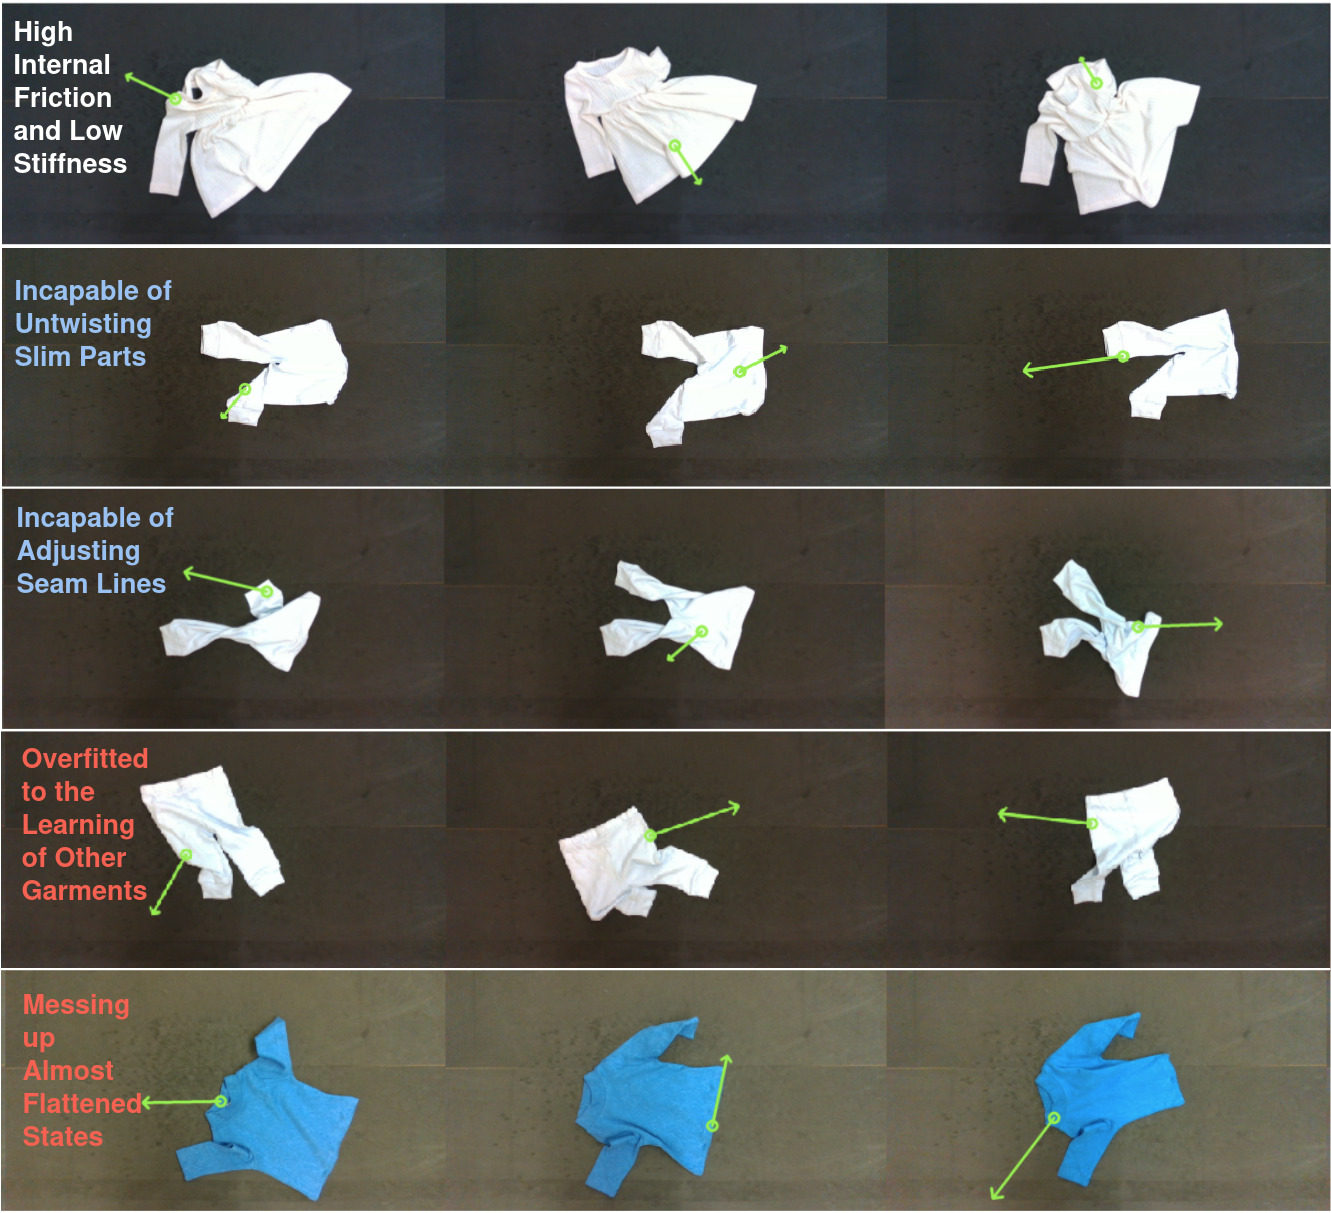
\includegraphics[width=1.0\linewidth]{plots/lagarnet-failure.jpg}
        \caption{Visual failure cases of LaGarNet.}
        \label{fig:failure-visuals}
    \end{subfigure}
    \hfill % Flexible space between left and right sides
    % --- RIGHT SIDE: Stacked Tables ---
    \begin{minipage}[t]{0.5\textwidth}
        \vspace{0pt} % CRITICAL: Matches the top baseline of the left subfigure
        
        % --- TOP RIGHT: Failure Modes (Subtable b) ---
        \begin{subtable}[t]{\linewidth}
            \centering
            \resizebox{\linewidth}{!}{% Auto-scales table to fit width
            \begin{tabular}{@{}llc@{}}
            \toprule
            \textbf{Failure Category} & \textbf{Specific Mode} & \textbf{Rate} \\ \midrule
            \multirow{3}{*}{\textbf{Trajectory}} 
            & Fold Underneath & 3/40 \\
            & Fold On the Top & 2/40 \\
            & Cannot untwist & 5/40 \\
            & Cannot stabilise on success state & 4/40 \\ \midrule
            \multirow{4}{*}{\textbf{Step-wise}} 
            & Segmentation failure & 1/800 \\
            & Misgrasping failure & 3/800 \\
            & Messing-near-success state & 168/298 \\
            & As-if-manipulating-other-object & 28/800 \\ \bottomrule
            \end{tabular}%
            }
            \caption{Trajectory and step-wise failure rates.}
            \label{tab:failure-rates}
        \end{subtable}
        
        \vspace{0.1in} % Vertical space between the top and bottom rows
        
        % --- BOTTOM ROW: Two Side-by-Side Tables ---
        
        % Bottom Left: Timing Metrics (Subtable c)
        \begin{subtable}[t]{0.52\linewidth}
            \centering
            \resizebox{\linewidth}{!}{% Auto-scales to fit the 0.48 width
            \begin{tabular}{@{}lc@{}}
\toprule
\textbf{System Phase} & \textbf{Time (s)} \\ \midrule
Perception & 8.19 \\
Action Inference & 7.05 \\
Action Conversion & 0.03 \\
Robot Execution & 9.20 \\ 
\bottomrule
\end{tabular}%
            }
            \caption{Average Time Consumption}
            \label{tab:timing_metrics}
        \end{subtable}
        \hfill % Pushes the two bottom tables to the edges
        % Bottom Right: Unseen Dress Metrics (Subtable d)
        \begin{subtable}[t]{0.4\linewidth}
            \centering
            \resizebox{\linewidth}{!}{% Auto-scales to fit the 0.48 width
            \begin{tabular}{@{}lc@{}}
\toprule
\textbf{Metric} & \textbf{Score} \\ \midrule
NC & 77.2 $\pm$ 6.5 \\
NI & 42.1 $\pm$ 22.6 \\
Max IoU & 66.4 $\pm$ 3.2 \\
SR & 0/10 \\
\bottomrule
\end{tabular}%
            }
            \caption{Unseen long-sleeve dress.}
            \label{tab:unseen-dress}
        \end{subtable}
        
    \end{minipage}
    
    \vspace{0.15in} % Space between the sub-elements and the main caption
    
    % --- GENERAL CAPTION FOR THE ENTIRE FIGURE* ---
    \caption{\addrealworld{Comprehensive analysis of LaGarNet's real-world performance. \textbf{(a)} Failure cases in the real world; text colours indicate the source of failure: white for mechanical limitations, blue for assumption oversights, and red for the learning process itself. \textbf{(b)} Quantitative analysis of failure modes. Note that a step-wise failure does not necessarily cause a trajectory failure; a trajectory is successful if it reaches the success state within 20 steps. ``Messing-near-success state'' is calculated through identifying  ``near-success'' steps (NC $\geq$ 0.8 and IoU $\geq$ 0.7) and calculates how often the performance drops in the very next step.\textbf{(c)} Breakdown of system timing metrics across the perception-action cycle. \textbf{(d)} Zero-shot generalisation metrics evaluated on an unseen longsleeved dress with soft material properties and high internal friction.}}
    \label{fig:real_world_analysis}
\end{figure*}


\subsubsection{Results}
\addrealworld{Table \ref{tab:real-worldflattening} demonstrates that the unified, all-garment version of LaGarNet can successfully flatten longsleeved T-shirts, trousers, skirts, and dresses in the real world, although it struggles with OOD garments (Table \ref{tab:unseen-dress}). LaGarNet shows substantial improvements over PlaNet-ClothPick. However, a significant performance gap remains compared to human baselines, particularly for garments with narrow appendages, such as longsleeved T-shirts and trousers.}

\addrealworld{Despite this gap, LaGarNet's performance is highly competitive within the field. Its NC and NI metrics surpass the reported state-of-the-art real-world performance for single-gripper garment flattening when compared to mesh-based planning methods like VCD \cite{lin2022learning} and MEDOR \cite{huang2022accelerating}. Furthermore, the results highlight a strong topology-dependent performance disparity: LaGarNet achieves a perfect 10/10 success rate for dresses and skirts within 20 steps, while the more complex dynamics of trousers and longsleeved shirts yield much lower success rates (3/10 and 4/10, respectively).}

\subsubsection{Limitations and Failure Cases}

\addrealworld{Despite its comparative success, LaGarNet encounters notable challenges in the real world. We observe a persistent simulation-to-reality (Sim2Real) gap, a phenomenon similarly documented in mesh-based planning literature \cite{huang2022mesh, lin2022learning}. We encounter typical multi-task learning capacity issues; training a unified all-garment policy leads to underfitting on complex topologies (longsleeved T-shirts and trousers) and overfitting on simpler ones (skirts and dresses), reflected in the performance disparities across garment types in Table \ref{tab:real-worldflattening}. Consequently, LaGarNet frequently fails to isolate and untwist narrow garment sections, such as sleeves and trouser legs. Trousers present an exceptional challenge, where the system frequently attempts to manipulate trouser legs as if they were T-shirt sleeves (see the ``As-if-manipulating-other-object'' error in Table \ref{tab:failure-rates}). Additionally, the policy occasionally disrupts already flattened garments; our GC-RSSM latent dynamics model cannot consistently predict the first-step prior reward accurately, leading to actions that degrade near-success states (see the  ``Messing-near-success stat'' in Table \ref{tab:failure-rates} and Figure \ref{fig:failure-visuals}).}

\addrealworld{Furthermore, our framework assumes that intrinsic physical properties (e.g., stiffness and elasticity) are secondary to geometric representations for high-level policy learning. Consequently, LaGarNet struggles with garments exhibiting high internal friction and low stiffness (Table \ref{tab:unseen-dress}). This is exacerbated by our single-arm, parallel-jaw gripper setup---a hardware constraint that limits the ability to unfold stubborn folds and wrinkles. In addition, distinguishing the front from the back of a garment was not defined as a task criterion. Consequently, LaGarNet cannot perform this semantic orientation---a cognitive spatial task known to be challenging even for young children \cite{paoletti2012pink}.}

\addrealworld{Finally, a critical limitation for practical deployment in fast-pacing garment factories is the system's time consumption. As detailed in Figure \ref{fig:real_world_analysis}(c), the perception phase (8.19 s) and action inference (7.05 s) create a substantial computational bottleneck. Combined with robot execution (9.20 s), a single manipulation step takes approximately 24.5 seconds. For a 20-step episode, this translates to over 8 minutes per garment. To scale this system for industrial or domestic applications, future work must prioritise optimising the latent dynamics model's inference speed and the perception processing pipeline.}

\section{Real Robot Setup} \label{sec:real-world-setup}

\addinfo{In cloth manipulation literature, robot arms are often fixed on a table  \cite{lin2022learning,lee2024learning,canberk2023cloth}, leading to a ring-shaped workspace for Pick-and-Place (PnP) primitives. Real garments are generally larger than simple fabrics, and it becomes physically impossible to flatten the garments on a fixed square window within the workspace of a single robot arm, which is \addinfo{a common practice in this domain \cite{kadi2025draper, hoque2022visuospatial, lee2021learning}}. Thereby, it requires us to develop a transfer strategy to bridge the gap between observation and the workspace in addition to the gap between the simulation and the real robot environment.}
\begin{figure*}[t!]
    \centering
    
    % --- Subpart (a): Real Robot Setup ---
    \begin{subfigure}[b]{0.3\linewidth}
        \centering
        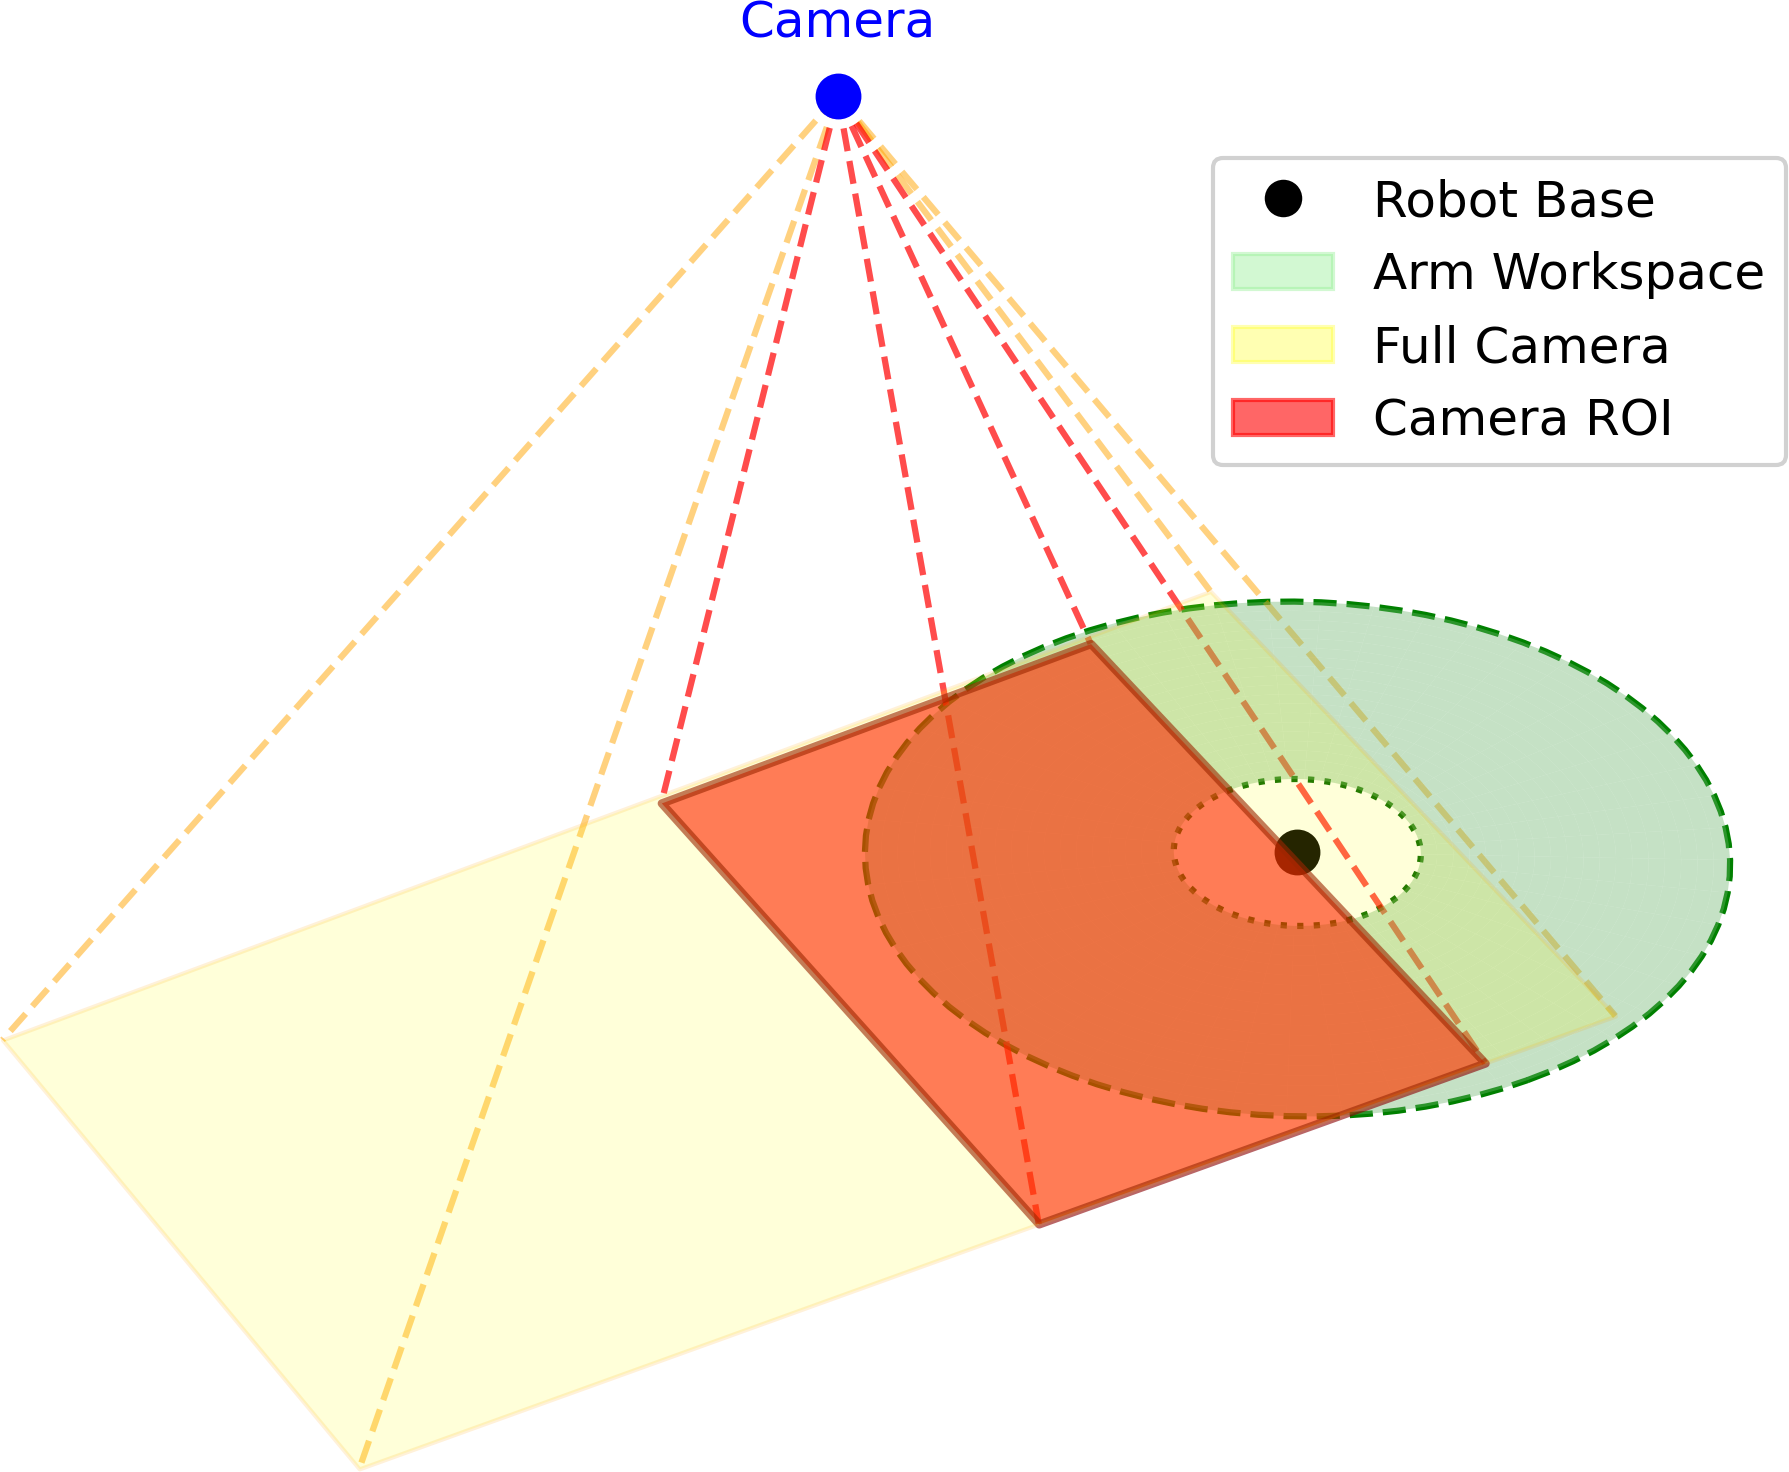
\includegraphics[width=\linewidth]{plots/tightest_cropped_plot.png}
        \caption{\addinfo{Camera Setup}}
        \label{fig:robot-camera}
    \end{subfigure}\hfill
    % --- Subpart (b): Transfer Heuristic ---
    \begin{subfigure}[b]{0.45\linewidth}
        \centering
        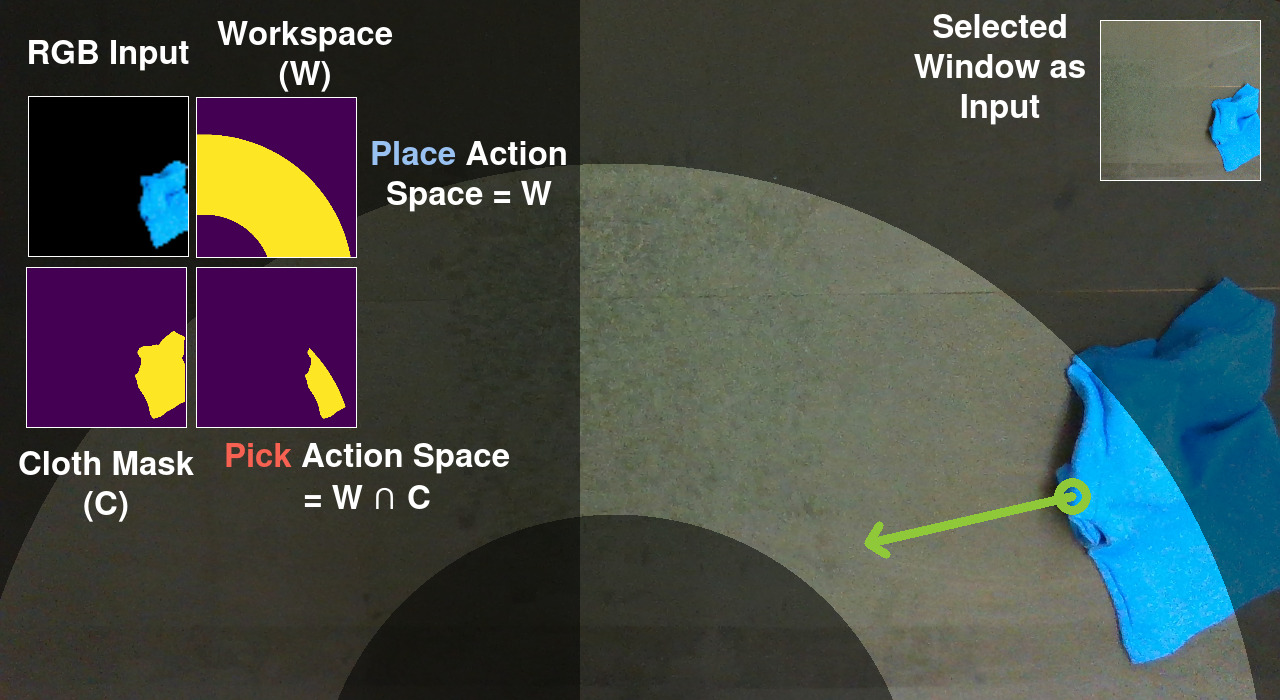
\includegraphics[width=\linewidth]{plots/transfer-hueristic-single.jpg}
        \caption{\addinfo{Heuristic of Transferring Policy in Region-of-Interest (ROI)}}
        \label{fig:transfer-hueristic}
    \end{subfigure}
    % --- Subpart (c): Segmentation Parameters Table ---
    \begin{subfigure}[b]{0.24\linewidth}
        \centering
        
        \label{fig:setup_c}
        \vspace{0.5em} % Small buffer between caption and table
        \resizebox{\textwidth}{!}{
        \begin{tabular}{lc}
        \toprule
        \textbf{Camera} & \textbf{Value} \\
        \midrule
        $FoV$ & 69$^\circ$ $\times$ 42$^\circ$\\
        Camera Resolution & 1280 $\times$ 720 px\\
        RoI Resolution & 450 $\times$ 710 px\\
        RoI Start & (700, 10) px \\
        $P_c$ & (0.03, -0.86, 1.66)m \\
        $r_n, rf$ & 0.7m, 0.2m\\
        \midrule
        \textbf{Segmentation} & \textbf{Value} \\
        \midrule
        model & \texttt{sam\_vit\_h\_4b8939} \\
        $A_{\text{min}}$  & $1,000$ \\
        $A_{\text{max}}$  & $90,000$ \\
        $\alpha_{border}$ & $0.15$\\
        $S_{\text{min}}$  & $10$ \\
        $V_{\text{min}}$ & $10$ \\
        \bottomrule
        \end{tabular}}
        \caption{\addinfo{Parameters} \label{tab:seg-para}}
    \end{subfigure}
    
    % --- Main Overarching Caption ---
    \caption{Overview of the real-world deployment setup. (a) \addinfo{Camera $P_c$ is set at the front of the robot and top of the table surface; whilst the camera can captures table view highlighted in yellow, our system operates on the Region-of-Interest (ROI) highlighted as red} (b) The heuristic approach for transferring the simulated policy to the real world; the heuristic prioritises the selection of the middle window for network inputs, but if the selected window does not contain any parts of the cloth, it re-select a window that centres around the cloth as shown; the most highlighted part on the rectangular images are the workspace of the \text{UR5e} Robot for a particular action step. (c) The empirical parameters utilised in the segmentation pipeline.}
    \label{fig:real-world-overview}
\end{figure*}
\addinfo{As shown in Figure \ref{fig:ur5e-onrobot}, we employ a UR5e robot arm equipped with an OnRobot RG2 electric parallel gripper to conduct our real-world experiments. We position a RealSense D435i camera $P_c$ in front of the robot and above a table covered with a dark foam surface. As in simulation, we use only RGB frames with automatic exposure as input to our method in the real-world setup.}

\addinfo{The workspace of our UR5e robot is defined by a far radius $r_{f}$ and a near radius $r_{n}$. To isolate the effective workspace, we crop the visual input to a Region of Interest (ROI) as in Figure \ref{fig:robot-camera}. Given the top-down camera perspective, we compute the spatial position $p_w$ in the world frame for each pixel $p_x$ in the camera view using the camera intrinsics and the transformation matrix. Consequently, we determine whether $p_x$ lies within the workspace by checking if $r_n \leq ||p_w - b_w||_2 \leq r_f$, where $b_w$ represents the position of the robot base in the world frame. Please refer to Table \ref{tab:seg-para} for the exact parameters of our real-robot setup.} \addinfo{We use UR-RTDE package \cite{urrtde2025} for conducting Cartesian planning for executing pick-and-place primitive, as they stably produce reliable trajectories.}

\addIncrementalg{This section first introduces the transfer heuristic, which integrates the real robot arm's workspace into LaGarNet's planning method (Section \ref{sec:transfer-hueristic}). Next, we discuss how we conduct our hand-eye calibration (Section \ref{sec:calibration}) for the transformation between the camera pixel space and robot base space. Then, we explain our approach to segmenting the physical garments from the camera observations (Section \ref{sec:real-world-cloth-seg}). Finally, we detail our grasping implementation, designed to ensure the precise and robust picking of garments (Section \ref{sec:grasping}).}

\subsection{Transfer Heuristic for Robot's Ring-Shaped Workspace} \label{sec:transfer-hueristic}
Many robot manipulators face workspace constraints, such as limited reach as well as undesirable trajectories caused by inverse kinematics and joint discontinuities. These factors often make parts of the workspace unusable for smooth pick-and-place (PnP) execution. To address this general class of problems, we propose a heuristic workspace sampling method that adapts trained policies to feasible regions of a robot’s workspace without retraining. We demonstrate this method on a \addtypo{UR5e} robot arm, whose PnP workspace resembles a ring due to both reach limitations and unstable trajectories near the base; the ring-like workspace is defined by a far radius $r_f$ and a near radius $r_n$ on the table surface.

% The \text{LaGarNet} algorithm proposed in the previous section cannot be employed directly in our real-robot setup, as the feasible square window for the pick-and-place (PnP) primitive is at most 28 cm $\times$ 28 cm for a \text{UR3e} robot arm, which is too small to flatten real garments. However, it is possible to utilise the entire ring-like workspace of the robot arm. 

% The workspace of a robot arm is often limited by its reach and the requirement to generate smooth PnP trajectories. In addition to the arm's maximum reach, we find that the workspace is also restricted by a smaller radius, within which motion planning algorithms produce trajectories that cause significant jumps in the robot arm's joint states when reaching its base. Hence, the PnP workspace of a robot arm resembles a ring

Our heuristic workspace sampling method (see Figure \ref{fig:transfer-hueristic}) builds an observation bridge between the \addtypo{UR5e} environment and the policy's training environment. This method prioritises the central square window of the raw RGB input. If the central window does not contain any part of the cloth, it re-selects a window centred on the target cloth. The \text{LaGarNet} latent dynamics network receives observations filtered by the cloth mask in the selected window, and the model predictive control planner samples pick actions at the intersection of the cloth mask and workspace mask, and place actions within the workspace mask in the selected window. Using these two processes, we ensure that \text{LaGarNet} can be transferred to the entire visible workspace of a \addtypo{UR5e} robot from a top-down camera for flattening real garments. \addrealworld{Note that the dynamic cropping mechanism of the transfer heuristic is only activated at the beginning of an episode if the garment is absent from the central field of view.}


\subsection{Hand-Eye Calibration} \label{sec:calibration}

\addinfo{To guarantee precise physical manipulation based on visual input, we conducted a rigorous eye-to-hand calibration to map the Intel RealSense camera's pixel space to the Universal Robots (UR) base frame. Our calibration target is a $5 \times 7$ ChArUco board \cite{garrido2014automatic} featuring 40~mm squares and 30.0~mm ArUco markers (Dictionary 4x4\_50) grasped by the robot's end-effector. To ensure an optimal and mathematically robust solution, we program the robot to traverse a trajectory of 50 carefully designed joint configurations. These poses explicitly sample the $SE(3)$ workspace, incorporating isolated Z-axis depth variations, lateral translations, and decoupled pitch, yaw, and roll rotations. This diverse pose generation prevents singularities and ensures the focal parameters are well-constrained. For each spatial sample, we estimate the target-to-camera transformation utilising a Perspective-n-Point solver based on the interpolated ChArUco corners. Finally, we compute the fixed camera-to-base transformation matrix by solving the standard $AX=XB$ formulation using the Park and Martin method \cite{park1994robot}.}




\subsection{Real-World Garment Segmentation} \label{sec:real-world-cloth-seg}
\addinfo{Following standard practices in the domain \cite{canberk2023cloth, lin2022learning, kadi2025draper}, we utilise the Segment Anything Model (SAM) \cite{kirillov2023segment} to isolate the target garment. This segmentation is crucial for stripping the background from policy inputs and enabling accurate real-world evaluation. Given an RGB observation, SAM generates a set of $K$ binary candidate masks. To efficiently isolate the true garment, we convert the image to the HSV color space and apply a multi-stage heuristic filtering pipeline. First, we apply spatial pruning: masks are retained only if their total pixel area $A \in [A_{\text{min}}, A_{\text{max}}]$. To eliminate broad background surfaces, we reject any candidate whose active border pixels exceed 30\% of the image perimeter, formalised as $P_{\text{mask}} > \alpha_{border} \times 2(h + w)$. Next, we apply chromatic and variance filters to distinguish the garment from its environment. For each mask, we compute the mean saturation $\bar{S}$ and RGB intensity variance $V$. We discard grey areas if $\bar{S} < S_{\text{min}}$ as low saturation. We further reject grey backgrounds by ensuring $ V \geq V_{min}$. Finally, the optimal mask is selected by maximising a utility score that prioritises large, distinctly coloured objects $\text{Score}_i = A_i \cdot \bar{V}_i$. This pipeline reliably yields high-fidelity garment segmentations for downstream manipulation tasks. The specific parameters used in our real-world experiments are detailed in Table \ref{tab:seg-para}.}
\subsection{Grasping} \label{sec:grasping}

\addinfo{Accurately grasping garments without failure remains a significant challenge for parallel grippers. We build upon the grasping protocol proposed by DRAPER \cite{kadi2025draper} which adjust the pick position on an eroded mask of the garment and ensures the axis connecting the two gripper fingers is perpendicular to the target mask cutline. However, while DRAPER utilises a custom pincher extension, our approach employs a standard OnRobot RG2 parallel gripper. To mitigate misgrasping errors, we initialised the gripper to a 3~cm opening width before the approach towards garments. The end-effector then executes a guarded descent, lowering gradually until the robot's force-torque sensor detects an upward reaction force of approximately 5~N. This force-based threshold ensures the garment is firmly contacted while preventing gripper faults or misgrasps caused by excessive collision resistance from the underlying workspace table.}


\section{Discussion} \label{sec:discussion}

The key reason for our investigation into latent dynamic representations is their potential to achieve generalisability across a broader range of contexts. By leveraging such representations, systems developed in this study may ultimately be extended beyond laboratory environments and applied in real-world scenarios, including everyday life and other discussed diverse settings. There are two critical challenges in applying RSSM in pick-and-place cloth shaping: (1) capturing the complex deformation of cloth objects and (2) quasi-static nature of high-level action primitive---the inferred states are not as  continuous as the ones in velocity/position-based control. We find that \text{RSSM} \cite{hafner2019learning} with its goal-conditioned extension is better at learning complex latent dynamics of cloth deformation caused by higher-level action primitives.

In general, offline reinforcement learning suffers from the problem of distribution shift \cite{prudencio2023survey}, where the testing trajectories misalign with those collected during training. Most of the offline RL literature relies on datasets collected using a single policy \cite{agarwal2020optimistic}. We find that the behaviour cloning method, \text{Diffusion Policy} \cite{chi2023diffusionpolicy}, can learn to flatten garments from only 50-200 human demonstrations. And, it can be used to collect data in the near-success distribution for offline RL algorithms, as it produces diverse actions around the expert-trajectory distribution. Building on this, our paper proposes a potentially generalisable data collection strategy for offline RL, which combines both a random policy and a learned diffusion policy from a view demonstration approach.

\addadvantage{Our offline model-based RL method, LaGarNet, demonstrates significant advantages over alternative approaches in the garment flattening domain. Firstly, LaGarNet is computationally more efficient than mesh-based planning methods, achieving comparable performance with fewer parameters and faster inference times. Furthermore, compared to both model-free and online RL methods, it exhibits greater data efficiency and yields more stable performance. LaGarNet also presents a distinct advantage over behaviour cloning (BC) methods, such as Diffusion Policy, as its policy is inherently explainable by predicting future outcomes on a given action, and it is not limited by the quality of the demonstration data. Crucially, BC relies on extensive expert demonstrations that are highly laborious to collect without an oracle or pre-trained demonstrator; for instance, gathering 200 episodes of 20-step trajectories requires approximately nine hours of human labour per garment type.}

\addadvantage{Beyond the data collection burden, BC methods often fail in unseen environments and face significant challenges during sim-to-real transfer. Although Diffusion Policy can solve the task with 200 demonstrations, adapting these policies to variable real-world scenarios is highly problematic. In our physical setup, workspace constraints fluctuate depending on where the heuristic method crops the raw RGB image. A Diffusion Policy trained without these exact constraints cannot be easily transferred, as enforcing workspace masks during action denoising is highly complex. Attempting to train a policy for all possible real-world variability would require an impractical amount of data. Conversely, LaGarNet natively handles these variations by constraining sampled actions directly within the workspace during the planning phase. Consequently, LaGarNet, even when trained with loose constraints in simulation, can seamlessly transfer to real-world setups with varying input constraints, entirely removing the need to retrain a simulated twin.}

\addIncremental{In summary, this research opens an exciting direction for applying state-space models to broader deformable object manipulation, such as handling dough, clay, or cables. State-space models can effectively encode the complex dynamics and high degrees of freedom of these objects into a latent space, thereby accelerating the planning and reasoning processes. While our current study focuses on reward-based planning for flattening, the model's future-feature prediction capabilities could potentially be extended to goal-directed folding.} 

%In future work, we intend to extend \text{LaGarNet} to achieve garment folding tasks with an improved learning and inference capability. We also aim to explore other action primitives, such as bimanual \text{pick-and-fling}, \text{pick-and-drag}, and hybrids of these actions \cite{avigal2022speedfolding,canberk2023cloth} to improve the versatility and efficiency of our system.  We also curious about the effectiveness of the proposed coverage-alignment reward in learning from real-world data. We also plan to investigate a transformer-based architecture \cite{deng2023facing} to replace the recurrent structure of our world model. The findings of the paper indicate that learning-based methods remain inferior to human-level manipulation under the same constraints. We speculate that one advantage humans possess is a strong understanding of the topological structures of various garment types. This naturally leads to new research questions: can neural controllers learn such topological structures of objects implicitly, enabling these controllers to achieve human-level manipulation?

\section{Conclusion} \label{sec:conclusion}

We introduce a general learning-based garment-flattening policy \text{LaGarNet} for single-arm pick-and-place (\text{PnP}) action primitives. It successfully flattens all four garment types with a single policy, including longsleeved T-shirt, trousers, skirts and dress, in both simulated and real-world environments. We achieve this through a more generalised goal-conditioned recurrent state-space model, a data-collection strategy and a coverage-alignment reward function. \text{LaGarNet} matches the state-of-the-art performance of mesh-based planning in garment flattening and human, marking the first successful application of state-space models on complex garments. \addIncremental{This research opens an exciting direction of applying state-space models in deformable object manipulation.} 

\section*{Acknowledgment}
We would like to thank the Institute of Safe Autonomy at the University of York for hosting the experimental evaluations, where \textbf{Dr James Hilder} and \textbf{Dr Rob Woolley} assist us to setup the robot platform. We also extend our gratitude to \textbf{Dr Stuart Norcross} at the University of St Andrews for providing access to essential GPU clusters. We also  acknowledge the use of the Viking cluster at York. We thank \textbf{Dr Ivan Kapelyukh} from Imperial College London for insightful discussions regarding the potential generalisation of this approach to dual manipulation and cloth folding. We acknowledge the use of Google's Gemini 3 Flash Image to remove the background and enhance the image quality of the experimental setup depicted in Figure 1(c). Furthermore, this work was supported by the Engineering and Physical Sciences Research Council, United Kingdom under grants: A digital COgnitive architecture to achieve Rapid Task programming and flEXibility in manufacturing robots through human demonstrations (DIGI-CORTEX), United Kingdom (EP/W014688/2)


\bibliographystyle{IEEEtran}
\bibliography{IEEEabrv,ref}

\end{document}
